\documentclass{../thunote}

% 各卷共用的数学记号。课程专用记号见相应的主入口。
\RequirePackage{amsmath,amssymb,bm,upgreek}

% 数集与函数空间
\newcommand*{\NN}{\mathbb{N}}
\newcommand*{\ZZ}{\mathbb{Z}}
\newcommand*{\QQ}{\mathbb{Q}}
\newcommand*{\RR}{\mathbb{R}}
\newcommand*{\CC}{\mathbb{C}}
\newcommand*{\FF}{\mathbb{F}}
\newcommand*{\cont}{\mathcal{C}}  % 连续函数空间，\cont^k 表示 k 次连续可微
\newcommand*{\poly}{\mathcal{P}}  % \poly_n 中多项式的次数至多为 n

% 微分与常数。文本中的无点 i 和字母下加点另有明确的命令。
\NewCommandCopy{\dotlessi}{\i}
\NewCommandCopy{\dotbelow}{\d}
\renewcommand*{\i}{\mathrm{i}}
\newcommand*{\nd}{\mathrm{d}}
\renewcommand*{\d}{\mathop{}\!\mathrm{d}}
\newcommand*{\e}{\mathop{}\!\mathrm{e}}
\newcommand*{\const}{\mathrm{const}}
\newcommand*{\vd}{\mathop{}\!\delta}  % 变分、依赖过程的热量或功的微元
\newcommand*{\p}{\partial}
\newcommand{\dd}[2][]{\frac{\d^{#1}}{\nd{#2}^{#1}}}
\newcommand{\dv}[3][]{\frac{\d^{#1}#2}{\nd{#3}^{#1}}}
\newcommand{\pp}[2][]{\frac{\p^{#1}}{\p{#2}^{#1}}}
\newcommand{\pv}[3][]{\frac{\p^{#1}#2}{\p{#3}^{#1}}}
\newcommand{\pw}[3]{\frac{\p^2{#1}}{\p{#2}\p{#3}}}

% 函数与算符
\let\Re\relax
\let\Im\relax
\DeclareMathOperator{\Re}{Re}
\DeclareMathOperator{\Im}{Im}
\DeclareMathOperator{\sech}{sech}
\DeclareMathOperator{\csch}{csch}
\DeclareMathOperator{\sinc}{sinc}
\DeclareMathOperator{\sgn}{sgn}
\DeclareMathOperator{\id}{id}
\DeclareMathOperator{\PV}{PV}
\DeclareMathOperator{\FT}{\mathcal{F}}
\DeclareMathOperator{\Beta}{B}
\DeclareMathOperator*{\argmin}{arg\,min}
\DeclareMathOperator*{\argmax}{arg\,max}
\newcommand*{\bigo}{\mathcal{O}}
\newcommand*{\intR}{\int_{-\infty}^\infty}
\newcommand*{\intRplus}{\int_0^\infty}

% 矢量、线性代数与场算符
\newcommand*{\hatbm}[1]{\hat{\bm{#1}}} % 带帽的粗体符号，含义随卷定义
\newcommand*{\dotbm}[1]{\dot{\bm{#1}}}
\newcommand*{\uvec}[1]{\mathop{}\!\hatbm{#1}}  % 系数后自动留薄空；单独取负写 -{\uvec n}
\newcommand*{\grad}{\nabla}
\renewcommand*{\div}{\nabla\cdot}
\newcommand*{\curl}{\nabla\times}
\newcommand*{\laplacian}{\nabla^2}
\DeclareMathOperator{\rank}{rank}
\DeclareMathOperator{\diag}{diag}
\DeclareMathOperator{\tr}{tr}
\DeclareMathOperator{\Span}{span}
\DeclareMathOperator{\nullsp}{N}
\DeclareMathOperator{\colsp}{C}
\newcommand*{\transp}{^\top}
\newcommand*{\conj}{^\ast}
\newcommand*{\adjoint}{^\dagger}
\newcommand*{\inv}{^{-1}}

% 概率、统计与物理量
\renewcommand*{\P}{\operatorname{P}}  % 段落符号 ¶ 可用 \textparagraph
\DeclareMathOperator{\E}{E}
\DeclareMathOperator{\Var}{Var}
\DeclareMathOperator{\BinDist}{Bin}
\DeclareMathOperator{\NormalDist}{N}
\newcommand*{\avg}[1]{\overline{#1}}
\newcommand*{\NA}{N_{\mathrm{A}}}
\newcommand*{\kB}{k_{\mathrm{B}}}
\newcommand*{\muB}{\mu_{\mathrm{B}}}
\newcommand*{\Ek}{E_{\mathrm{k}}}
\newcommand*{\FWHM}{\mathrm{FWHM}}
\newcommand*{\electron}{\mathrm{e}}       % 粒子标签，如 m_\electron
\newcommand*{\proton}{\mathrm{p}}
\newcommand*{\nucleus}{\mathrm{N}}
\newcommand*{\excitedstate}{\mathrm{e}}
\newcommand*{\groundstate}{\mathrm{g}}
\newcommand*{\CM}{\mathrm{CM}}
\newcommand*{\transv}{\mathrm t}  % 横向分量或模式的标签
\newcommand*{\longit}{\mathrm l}  % 纵向分量或模式的标签
\newcommand*{\electric}{\mathrm e}
\newcommand*{\magnetic}{\mathrm m}
\newcommand*{\incident}{\mathrm i}
\newcommand*{\initial}{\mathrm i}
\newcommand*{\final}{\mathrm f}
\newcommand*{\hi}{\mathrm{hi}}
\newcommand*{\lo}{\mathrm{lo}}
\newcommand*{\eff}{\mathrm{eff}}
\newcommand*{\tot}{\mathrm{tot}}

% 括号与 Dirac 记号。显式声明让公式预览也能读到每个尺寸的命令。
\newcommand{\abs}[1]{\lvert#1\rvert}
\newcommand{\bigabs}[1]{\bigl\lvert#1\bigr\rvert}
\newcommand{\Bigabs}[1]{\Bigl\lvert#1\Bigr\rvert}
\newcommand{\biggabs}[1]{\biggl\lvert#1\biggr\rvert}
\newcommand{\Biggabs}[1]{\Biggl\lvert#1\Biggr\rvert}

\newcommand{\norm}[1]{\lVert#1\rVert}
\newcommand{\bignorm}[1]{\bigl\lVert#1\bigr\rVert}
\newcommand{\Bignorm}[1]{\Bigl\lVert#1\Bigr\rVert}
\newcommand{\biggnorm}[1]{\biggl\lVert#1\biggr\rVert}
\newcommand{\Biggnorm}[1]{\Biggl\lVert#1\Biggr\rVert}

\newcommand{\eval}[1]{{#1}\rvert}
\newcommand{\bigeval}[1]{{#1}\bigr\rvert}
\newcommand{\Bigeval}[1]{{#1}\Bigr\rvert}
\newcommand{\biggeval}[1]{{#1}\biggr\rvert}
\newcommand{\Biggeval}[1]{{#1}\Biggr\rvert}

\newcommand{\floor}[1]{\lfloor#1\rfloor}
\newcommand{\bigfloor}[1]{\bigl\lfloor#1\bigr\rfloor}
\newcommand{\Bigfloor}[1]{\Bigl\lfloor#1\Bigr\rfloor}
\newcommand{\biggfloor}[1]{\biggl\lfloor#1\biggr\rfloor}
\newcommand{\Biggfloor}[1]{\Biggl\lfloor#1\Biggr\rfloor}

\newcommand{\ceil}[1]{\lceil#1\rceil}
\newcommand{\bigceil}[1]{\bigl\lceil#1\bigr\rceil}
\newcommand{\Bigceil}[1]{\Bigl\lceil#1\Bigr\rceil}
\newcommand{\biggceil}[1]{\biggl\lceil#1\biggr\rceil}
\newcommand{\Biggceil}[1]{\Biggl\lceil#1\Biggr\rceil}

\newcommand{\ave}[1]{\langle#1\rangle}
\newcommand{\bigave}[1]{\bigl\langle#1\bigr\rangle}
\newcommand{\Bigave}[1]{\Bigl\langle#1\Bigr\rangle}
\newcommand{\biggave}[1]{\biggl\langle#1\biggr\rangle}
\newcommand{\Biggave}[1]{\Biggl\langle#1\Biggr\rangle}

\newcommand{\set}[2]{\{#1\,\vert\,#2\}}
\newcommand{\bigset}[2]{\bigl\{#1\,\big\vert\,#2\bigr\}}
\newcommand{\Bigset}[2]{\Bigl\{#1\,\Big\vert\,#2\Bigr\}}
\newcommand{\biggset}[2]{\biggl\{#1\,\bigg\vert\,#2\biggr\}}
\newcommand{\Biggset}[2]{\Biggl\{#1\,\Bigg\vert\,#2\Biggr\}}

\newcommand{\division}[2]{{#1}/{#2}}
\newcommand{\bigdivision}[2]{{#1}\big/{#2}}
\newcommand{\Bigdivision}[2]{{#1}\Big/{#2}}
\newcommand{\biggdivision}[2]{{#1}\bigg/{#2}}
\newcommand{\Biggdivision}[2]{{#1}\Bigg/{#2}}

\newcommand{\inp}[2]{\langle#1,#2\rangle}
\newcommand{\biginp}[2]{\bigl\langle#1,#2\bigr\rangle}
\newcommand{\Biginp}[2]{\Bigl\langle#1,#2\Bigr\rangle}
\newcommand{\bigginp}[2]{\biggl\langle#1,#2\biggr\rangle}
\newcommand{\Bigginp}[2]{\Biggl\langle#1,#2\Biggr\rangle}

\newcommand{\bra}[1]{\langle#1\rvert}
\newcommand{\bigbra}[1]{\bigl\langle#1\bigr\rvert}
\newcommand{\Bigbra}[1]{\Bigl\langle#1\Bigr\rvert}
\newcommand{\biggbra}[1]{\biggl\langle#1\biggr\rvert}
\newcommand{\Biggbra}[1]{\Biggl\langle#1\Biggr\rvert}

\newcommand{\ket}[1]{\lvert#1\rangle}
\newcommand{\bigket}[1]{\bigl\lvert#1\bigr\rangle}
\newcommand{\Bigket}[1]{\Bigl\lvert#1\Bigr\rangle}
\newcommand{\biggket}[1]{\biggl\lvert#1\biggr\rangle}
\newcommand{\Biggket}[1]{\Biggl\lvert#1\Biggr\rangle}

\newcommand{\braket}[2]{\langle#1\vert#2\rangle}
\newcommand{\bigbraket}[2]{\bigl\langle#1\big\vert#2\bigr\rangle}
\newcommand{\Bigbraket}[2]{\Bigl\langle#1\Big\vert#2\Bigr\rangle}
\newcommand{\biggbraket}[2]{\biggl\langle#1\bigg\vert#2\biggr\rangle}
\newcommand{\Biggbraket}[2]{\Biggl\langle#1\Bigg\vert#2\Biggr\rangle}

\newcommand{\mel}[3]{\langle#1\vert#2\vert#3\rangle}
\newcommand{\bigmel}[3]{\bigl\langle#1\big\vert#2\big\vert#3\bigr\rangle}
\newcommand{\Bigmel}[3]{\Bigl\langle#1\Big\vert#2\Big\vert#3\Bigr\rangle}
\newcommand{\biggmel}[3]{\biggl\langle#1\bigg\vert#2\bigg\vert#3\biggr\rangle}
\newcommand{\Biggmel}[3]{\Biggl\langle#1\Bigg\vert#2\Bigg\vert#3\Biggr\rangle}

\newcommand{\ketbra}[2]{\lvert#1\rangle\langle#2\rvert}
\newcommand{\bigketbra}[2]{\bigl\lvert#1\bigr\rangle\bigl\langle#2\bigr\rvert}
\newcommand{\Bigketbra}[2]{\Bigl\lvert#1\Bigr\rangle\Bigl\langle#2\Bigr\rvert}
\newcommand{\biggketbra}[2]{\biggl\lvert#1\biggr\rangle\biggl\langle#2\biggr\rvert}
\newcommand{\Biggketbra}[2]{\Biggl\lvert#1\Biggr\rangle\Biggl\langle#2\Biggr\rvert}

% 兼容旧版笔记中的内积与外积命令。
\let\brkt\braket
\let\bigbrkt\bigbraket
\let\Bigbrkt\Bigbraket
\let\biggbrkt\biggbraket
\let\Biggbrkt\Biggbraket
\let\ktbr\ketbra
\let\bigktbr\bigketbra
\let\Bigktbr\Bigketbra
\let\biggktbr\biggketbra
\let\Biggktbr\Biggketbra

\newcommand{\bigp}[1]{\bigl(#1\bigr)}
\newcommand{\Bigp}[1]{\Bigl(#1\Bigr)}
\newcommand{\biggp}[1]{\biggl(#1\biggr)}
\newcommand{\Biggp}[1]{\Biggl(#1\Biggr)}

\newcommand{\bigb}[1]{\bigl[#1\bigr]}
\newcommand{\Bigb}[1]{\Bigl[#1\Bigr]}
\newcommand{\biggb}[1]{\biggl[#1\biggr]}
\newcommand{\Biggb}[1]{\Biggl[#1\Biggr]}

\newcommand{\bigB}[1]{\bigl\{#1\bigr\}}
\newcommand{\BigB}[1]{\Bigl\{#1\Bigr\}}
\newcommand{\biggB}[1]{\biggl\{#1\biggr\}}
\newcommand{\BiggB}[1]{\Biggl\{#1\Biggr\}}

% 公式排版
% 方程组的内容是一个 aligned 块，左花括号随整组方程的高度伸展。
\newcommand{\eqnset}[1]{\left\{#1\right.}
\newcommand{\fracdisp}[2]{\frac{\displaystyle #1}{\displaystyle #2}}
\newcommand*{\vs}{\mathord{\text{–}}}
\newcommand*{\otherwise}{\text{otherwise}}
\newcommand*{\qqquad}{\qquad\quad}
\newcommand*{\qqqquad}{\qquad\qquad}

\renewcommand*{\le}{\leqslant}
\renewcommand*{\leq}{\leqslant}
\renewcommand*{\ge}{\geqslant}
\renewcommand*{\geq}{\geqslant}

\externaldocument[tikz:]{figures/tikz}

% 矩阵范数与条件数
\newcommand*{\frobnorm}[1]{\norm{#1}_{\mathrm F}}
\DeclareMathOperator{\cond}{cond}

\title{数值分析\\Numerical Analysis}

\begin{document}
\maketitle

\frontmatter
\tableofcontents

\mainmatter
\chapter{数学基础知识}
\label{chap:math basics}

\section{线性空间}
\label{sec:linear space}

\subsection{线性空间}

\begin{definition}
    {线性空间}{linear space}
    给定一个数域$\FF$ (本笔记只涉及实数域$\RR$和复数域$\CC$)和一个集合$V$，
    
    定义加法$+:V \times V \to V$满足：
    \begin{itemize}
        \item 结合律：$(a + b) + c = a + (b + c),$
        \item 零元：$a + 0 = a,$
        \item 逆元：$a + (-a) = 0,$
        \item 交换律：$a + b = b + a;$
    \end{itemize}
    数乘$\cdot :\FF \times V \to V$满足：
    \begin{itemize}
        \item 单位元：$1a = a,$
        \item 结合律：$(\lambda\mu)a = \lambda(\mu a),$
        \item 分配率1：$(\lambda + \mu)a = \lambda a + \mu a,$
        \item 分配率2：$\lambda(a + b) = \lambda a + \lambda b.$
    \end{itemize}
    则称$V$在$\FF$上构成一个线性空间(linear space)。
\end{definition}

\begin{example}
    {线性空间的例子}{}
    \begin{itemize}
        \item $\cont^n$：全体在$\RR$上$n$次导数连续(continuous)的函数构成的集合。
        \item $\poly_n = \set{x \mapsto a_0 + a_1x + \cdots + a_nx^n}{a_i \in \FF}$：系数在 $\FF$ 中、次数不超过 $n$ 的多项式构成的空间（含零多项式）。
        % \item 正实数$\RR_{>0}$构成一个线性空间，其加法为实数乘法，数乘为幂次。
    \end{itemize}
\end{example}

\subsection{线性空间的基和维度}

\begin{definition}
    {线性无关}{linear independent}
    设$V$是线性空间，给定其中$n$个元素$x_1,\ldots,x_n \in V$，若%其线性组合(linear combination)
    \begin{equation}
        a_1x_1 + \cdots + a_nx_n = 0 \iff a_1 = \cdots = a_n = 0,
    \end{equation}
    则称$x_1,\ldots,x_n$线性无关(linear independent)，否则称为线性相关。
\end{definition}

\begin{example}
    {线性无关的例子}{}
    \begin{itemize}
        \item $\poly_n$中$\{1,x,\ldots,x^n\}$是线性无关的；
        \item 所有$[-\pi,\pi]$上的周期函数构成的函数空间是线性空间，其中
        \[
            \{1,\cos x,\sin x,\ldots,\cos nx,\sin nx\} 
        \]
        线性无关。
    \end{itemize}
\end{example}

\begin{definition}
    {线性空间的基和维度}{dimension, base}
    给定线性空间$V$中的一组元素$\{x_1,\ldots,x_n\}$，若$\forall x \in V$都可以被唯一表示为其线性组合
    \begin{equation}
        x = a_1x_1 + \cdots + a_nx_n,
    \end{equation}
    则称$\{x_1,\ldots,x_n\}$构成一组基(base)，且$V$的维度$\dim(V) = n$。
\end{definition}

\begin{theorem}
    {}{}
    线性空间的维度与基的选取没有关系。
\end{theorem}

\begin{example}
    {典型线性空间的维度}{}
    \begin{itemize}
        \item $\dim(\poly_n) = n + 1;$
        \item $\dim(\cont) = +\infty.$
    \end{itemize}
\end{example}

\section{范数}
\label{sec:norm}

\subsection{度量空间}

\begin{definition}
    {度量空间}{metric space}
    给定集合$M$，若映射$d:M \times M \to \RR$满足：
    $\forall x,y \in M$
    \begin{itemize}
        \item 正定性：$d(x,y) \geq 0$，且$d(x,y) = 0 \iff x = y$；
        \item 交换性：$d(x,y) = d(y,x)$；
        \item 三角不等式：$d(x,y) + d(y,z) \geq d(x,z)$。
    \end{itemize}
    则称$M$是一个度量空间(metric space)或距离空间，$d$为度量函数或距离函数。
\end{definition}

\begin{definition}
    {Cauchy序列}{Cauchy sequence}
    对于序列$\{x_n\}$，若$\forall\varepsilon > 0,\exists N \in \NN$满足：
    \begin{equation}
        d(x_m,x_n) < \varepsilon,\quad\forall m,n > N,
    \end{equation}
    则称$\{x_n\}$为Cauchy序列(Cauchy sequence)。
\end{definition}

\begin{definition}
    {度量空间的完备性}{completeness}
    若$\forall$ Cauchy序列$\{x_n\} \subset M$，$\exists x \in M$满足：
    \begin{equation}\label{eq:na-metric-convergence}
        \lim_{n\to\infty}d(x_n,x) = 0,\quad(\text{记作}\lim_{n\to\infty}x_n = x)
    \end{equation}
    则称度量空间$M$是完备的(complete)。
\end{definition}

\begin{remark}
    不严谨地说，完备性要求：所有在$M$中收敛的序列都会收敛到$M$中。%即$M$中没有“缺失点”。
\end{remark}

\begin{example}
    {实数公理}{}
    实数集$\RR$中的度量函数$d(a,b) = |a - b|$是完备的。
\end{example}

\begin{remark}
    有理数域$\QQ$中的度量函数$d(a,b) = \abs{a - b}$不是完备的，比如
    \[
        x_0 = 1,\enspace x_{n+1} = \frac{x_n}2 + \frac1{x_n} \to \sqrt2 \notin \QQ.
    \]
\end{remark}

\begin{theorem}
    {完备化定理}{}
    若$(M,d)$是一个度量空间，则存在唯一等距同构的完备化空间。%一个从$M$到一个完备度量空间的等距嵌入。
\end{theorem}

\begin{proof}
    构造性证明：令$\tilde M$是$M$中所有Cauchy序列$\{x_n\}$的集合。在$\tilde M$中定义等价关系：
    \begin{equation}\label{eq:na-cauchy-sequence-equivalence}
        \{x_n\} \sim \{y_n\} \iff \lim_{n\to\infty}d(x_n,y_n) = 0.
    \end{equation}
    令$[\{x_n\}] = \set{\{y_n\} \in \tilde M}{\{x_n\} \sim \{y_n\}}$表示$\{x_n\}$的等价类，$\hat M = \set{[\{x_n\}]}{\{x_n\} \in \tilde M}$是$M$中所有Cauchy序列的等价类构成的集合。定义$\hat M$上的度量为
    \begin{equation}\label{eq:na-completion-metric}
        \hat d([\{x_n\}],[\{y_n\}]) := \lim_{n\to\infty}d(x_n,y_n),
    \end{equation}
    可证$(\hat M,\hat d)$是完备的度量空间。且存在等距嵌入
    \begin{equation}\label{eq:na-completion-embedding}
        i:M \to \hat M,\enspace x \mapsto [\{x,x,\ldots\}].
    \end{equation}
    即$i$是映射到对应常数序列的等价类。
\end{proof}

\subsection{赋范空间与范数}

\begin{definition}
    {赋范空间与范数}{normed space}
    给定数域$\FF$上的线性空间$V$，若映射$\norm \cdot :V \to \RR$满足：$\forall a,b \in V,\lambda \in \FF$
    \begin{itemize}
        \item 正定性：$\norm a \geq 0$，且$\norm a = 0 \iff a = 0$；
        \item 齐次性：$\norm{\lambda a} = \abs\lambda\norm a$；
        \item 三角不等式：$\norm{a + b} \leq \norm a + \norm b$。
    \end{itemize}
    则称$(V,\norm \cdot)$构成一个赋范空间(normed space)，$\norm \cdot$是$V$的范数(norm)。
\end{definition}

\begin{corollary}
    显然，赋范空间也是度量空间，只需定义$d(a,b) := \norm{a - b}$即可。
\end{corollary}
\begin{remark}
    赋范空间不一定是完备的，完备的赋范空间称为Banach空间。
\end{remark}

\begin{example}
    {$\RR^n$的$p$-范数}{vector p-norm}
    向量$x = (x_1,\ldots,x_n)\transp \in \FF^n$的$p$-范数为
    \begin{equation}
        \label{eqn:p-norm vector}
        \norm x_p = \biggp{\sum_{i=1}^n\abs{x_i}^p}^{1/p},
        \quad p > 0.
        % =\begin{cases}
        %     \max_{i}\abs{x_i},&p=\infty\\
        %     \sum_{i=1}^n\abs{x_i},&p=1\\
        %     \biggp{\sum_{i=1}^n\abs{x_i}^2}^{1/2},&p=2
        % \end{cases}
    \end{equation}
    当$p \to \infty$时，$p$-范数趋于最大分量的绝对值：
    \begin{equation}\label{eq:na-infinity-vector-norm}
        \norm x_\infty = \lim_{p\to\infty}\norm x_p = \max_i\abs{x_i}.
    \end{equation}
    \begin{proof}
        记$\textstyle k = \argmax_i\abs{x_i}$，对下式两边开$p$次方并令$p \to \infty$即得
        \[
            \abs{x_k}^p \leq \sum_{i=1}^n\abs{x_i}^p \leq n\abs{x_k}^p.
            \qedhere
        \]
    \end{proof}
    \tcblower
    二维位置向量$r = (x,y) \in \RR^2$，方程$\norm r_p = 1$在直角坐标中的图像为
    \begin{notecaptionblock}
        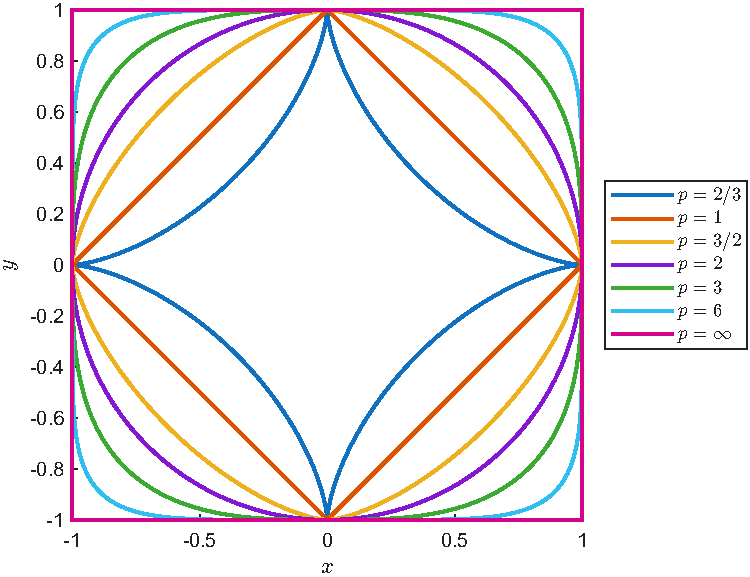
\includegraphics[width=0.7\linewidth]{figures/Lpspace.pdf}
        \captionof{figure}{不同的$p$-范数}
        \label{fig:Lp space}
    \end{notecaptionblock}
    特别地，$p = 2/3$的曲线叫星形线(astroid)。
\end{example}

\begin{example}
    {$C[a,b]$的$p$-范数}{function p-norm}
    函数$f \in \cont[a,b]$的$p$-范数为
    \begin{equation}
        \label{eqn:p-norm function}
        \norm f_p = \biggp{\int_a^b\abs{f(x)}^p\d x}^{1/p},
        % =\begin{cases}
        %     \max_{a\leq x\leq b}\abs{f(x)},&p=\infty\\
        %     \int_a^b\abs{f(x)}\d x,&p=1\\
        %     \biggp{\int_a^b\abs{f(x)}^2\d x}^{1/2},&p=2
        % \end{cases}
    \end{equation}
    当$1 < p < \infty$时，$\norm \cdot_p$是不完备的，
    \footnote{连续函数的Cauchy序列可以按$p$-范数收敛于一个不连续的函数}
    但$\norm \cdot_\infty$是完备的。
\end{example}

\subsection{范数的等价性}

\begin{definition}
    {范数的等价性}{}
    给定线性空间$V$上的两个范数$\norm \cdot_\alpha,\norm \cdot_\beta$，若$\exists C_1,C_2 > 0$满足：
    \begin{equation}\label{eq:na-equivalent-norms}
        C_1\norm x_\alpha \leq \norm x_\beta \leq C_2\norm x_\alpha,
    \end{equation}
    则称$\norm \cdot_\alpha,\norm \cdot_\beta$等价(equivalent)。
\end{definition}

\begin{corollary}
    向量的$p$-范数都是等价的，因为由H\"older不等式，$p < q$时
    \begin{equation}
        \norm x_q \leq \norm x_p \leq n^{1/p-1/q}\norm x_p.
    \end{equation}
\end{corollary}

\begin{theorem}
    {}{}
    有限维线性空间中，任意两个范数都是等价的。
\end{theorem}


\section{内积}
\label{sec:inner product}

\begin{definition}
    {内积}{inner product}
    给定线性空间$V$，内积(inner product)是一个映射$\inp \cdot \cdot :V \times V \to \FF$，
    满足：
    \begin{itemize}
        \item 正定性：$\inp xx \geq 0$，且$\inp xx = 0 \iff x = 0;$
        \item 交换共轭：$\inp xy = \overline{\inp yx};$
        \item 对第一个变量线性：$\inp{ax + by}z = a\inp xz + b\inp yz.$
    \end{itemize}
    若$\inp xy = 0$，则称$x,y$是正交的(orthogonal)。
\end{definition}

\begin{remark}
    对第二个变量不一定线性，会出现复共轭：
    \begin{equation}\label{eq:na-conjugate-linearity}
        \inp x{ay + bz} = \overline a\inp xy + \overline b\inp xz.
    \end{equation}
    除非内积的值域$\FF \subset \RR$，此时内积满足对称性：$\inp xy = \inp yx$。
\end{remark}

\begin{corollary}
    根据内积可以自然定义出一个范数，称为内积诱导的范数：
    \begin{equation}
        \norm x := \sqrt{\inp xx},
    \end{equation}
    因此内积空间也是赋范空间，完备的内积空间称为Hilbert空间。
\end{corollary}

\begin{example}
    {内积实例}{}
    \begin{itemize}
        \item $\CC^n$中的标准内积为
        \begin{equation}\label{eq:na-complex-inner-product}
            \inp xy = \sum_{i=1}^nx_i\overline y_i,
        \end{equation}
        标准内积诱导出来的范数就是2-范数。
        \item $\cont[a,b]$的带权内积为 
        \begin{equation}\label{eq:na-weighted-inner-product}
            \inp fg = \int_a^bf(x)\overline g(x)\rho(x)\d x.
        \end{equation}
        其中$\rho \in \cont(a,b)$是一个几乎处处为正的函数，\footnote{即$\{x|\rho(x) \leq 0\}$的Lebesgue测度为0。}且在$[a,b]$上积分有限。
    \end{itemize}
\end{example}

\begin{theorem}
    {Cauchy--Schwarz不等式}{Cauchy-Schwarz inequality}
    设$V$是内积空间，则$\forall x,y \in V$，有
    \begin{equation}
        \abs{\inp xy}^2 \leq \inp xx\inp yy,
    \end{equation}
    等号成立当且仅当$x,y$线性相关。
\end{theorem}

\begin{proof}
    当$y = 0$时显然成立，当$y \neq 0$时，考虑
    \[
        \biggnorm{x - \frac{\inp xy}{\inp yy}y}^2 = \inp xx - \frac{\abs{\inp xy}^2}{\inp yy} \geq 0.
        \qedhere
    \]
\end{proof}

\begin{definition}
    {Gram矩阵}{Gram matrix}
    给定一组向量$x_1,\ldots,x_n$，Gram矩阵的元素由内积给出：$G_{ij} = \inp{x_i}{x_j}$
    \begin{equation}
        G := \begin{bmatrix}
            \inp{x_1}{x_1}&\cdots&\inp{x_1}{x_n}\\
            \vdots&\ddots&\vdots\\
            \inp{x_n}{x_1}&\cdots&\inp{x_n}{x_n}
        \end{bmatrix}.
    \end{equation}
\end{definition}

\begin{corollary}
    由于内积交换共轭$\inp{x_i}{x_j} = \overline{\inp{x_j}{x_i}}$，Gram矩阵是Hermite的：$G\adjoint = G$。
\end{corollary}

\begin{theorem}
    {内积空间线性无关的判定}{}
    $x_1,\ldots,x_n$线性无关$\iff$ Gram矩阵可逆。
\end{theorem}

\begin{proof}
    考虑$aG = 0$，则$\forall k = 1,\ldots,n$
    \[
        (aG)_k = a_1\inp{x_1}{x_k} + \cdots + a_n\inp{x_n}{x_k} = \inp{a_1x_1 + \cdots + a_nx_n}{x_k} = 0,
    \]
    特别地，
    \[
        \inp{a_1x_1 + \cdots + a_nx_n}{a_1x_1 + \cdots + a_nx_n} = 0 \iff a_1x_1 + \cdots + a_nx_n = 0,
    \]
    则$G$可逆$\iff \nullsp(G\transp) = \{0\} \iff a$只有零解。
\end{proof}

\begin{example}
    {正交基}{}
    给定内积空间$V$的一组基$\{x_1,\ldots,x_n\}$，则$\forall x \in V$均可以写成
    \[
        x = a_1x_1 + \cdots + a_nx_n,
    \]
    下面求$a_1,\ldots,a_n$：两边分别与$x_i$做内积可得
    \[
        \inp x{x_i} = a_1\inp{x_1}{x_i} + \cdots + a_n\inp{x_n}{x_i},
    \]
    即
    \[
        [\inp x{x_1}\enspace\cdots\enspace\inp x{x_n}] = [a_1\enspace\cdots\enspace a_n]G,
    \]
    若基是正交的，即$\forall i \neq j,\enspace\inp{x_i}{x_j} = 0$，Gram矩阵是对角的，此时
    \begin{equation}\label{eq:na-orthogonal-coordinates}
        a_i = \frac{\inp x{x_i}}{\inp{x_i}{x_i}}.
    \end{equation}
\end{example}

\begin{theorem}
    {Schmidt正交化}{}
    设$x_1,\ldots,x_n$是一组线性无关的基，为得到一组正交基，定义
    \begin{equation}
        y_i = x_i - \sum_{j=1}^{i-1}\frac{\inp{x_i}{y_j}}{\inp{y_j}{y_j}}y_j.
    \end{equation}
    则$y_1,\ldots,y_n$是正交的。
\end{theorem}

\begin{definition}
    {正交多项式}{}
    已知$\{1,x,\ldots,x^n\}$是线性无关的。考虑$\cont[a,b]$上的带权内积，Schmidt正交化得到一组多项式函数
    \[
        \psi_0(x),\psi_1(x),\ldots,\psi_n(x),
    \]
    显然，$\deg(\psi_i) = i.$
\end{definition}

\begin{example}
    {Legendre多项式}{Legendre polynomial}
    权函数$\rho = 1$，区间$[-1,1]$，得到Legendre多项式
    \begin{equation}
        P_n(x) = \frac1{2^nn!}\dd[n]x(x^2 - 1)^n.
    \end{equation}
    性质：
    \begin{itemize}
        \item 内积 
        \begin{equation}
            \inp{P_n}{P_m} = \frac2{2n + 1}\delta_{nm}.
        \end{equation}
        \item 递归关系
        \begin{equation}
            (n + 1)P_{n+1}(x) = (2n + 1)xP_n(x) - nP_{n-1}(x).
        \end{equation}
        \item 奇偶性
        \begin{equation}
            P_n(-x) = (-1)^nP_n(x).
        \end{equation}
    \end{itemize}
\end{example}

\begin{example}
    {Chebyshev多项式}{Chebyshev polynomial}
    权函数$\rho(x) = (1 - x^2)^{-1/2}$，区间$[-1,1]$，得到Chebyshev多项式
    \begin{equation}
        T_n(x) = \cos(n\arccos x).
    \end{equation}
    性质：
    \begin{itemize}
        \item 内积 
        \begin{equation}
            \inp{T_n}{T_n} = \begin{cases}
                \pi,&n = 0\\
                \pi/2,&n \geq 1
            \end{cases}
        \end{equation}
        \item 递推关系
        \begin{equation}
            T_{n+1}(x) = 2xT_n(x) - T_{n-1}(x).
        \end{equation}
        \item 奇偶性
        \begin{equation}
            T_n(-x) = (-1)^nT_n(x);
        \end{equation}
        \item $T_n$的$n$个实单根为$\cos\bigb{(2k - 1)\pi/2n}$，$(n + 1)$个极值点为$\cos(k\pi/n)$
        \item 当$\abs x \geq 1$时，
        \begin{equation}
            T_n(x) = \frac12\biggb{\Bigp{x + \sqrt{x^2 - 1}}^n + \Bigp{x - \sqrt{x^2 - 1}}^n}.
        \end{equation}
    \end{itemize}
\end{example}

\section{矩阵空间}
\label{sec:matrix space}

\subsection{矩阵范数}

\begin{definition}
    {矩阵范数}{matrix norm}
    矩阵空间上的范数$\norm \cdot :\FF^{n\times n} \to \RR$若满足
    \begin{equation}
        \norm{AB} \leq \norm A\norm B,
    \end{equation}
    则$\norm \cdot$称为矩阵范数(matrix norm)。
\end{definition}


\begin{example}
    {Frobenius范数}{Frobenius norm}
    定义Frobenius范数
    \begin{equation}
        \frobnorm A := \sqrt{\sum_{i=1}^n\sum_{j=1}^n\abs{A_{ij}}^2}.
    \end{equation}
    是一个矩阵范数。
    \begin{proof}
        由Cauchy--Schwarz不等式
        \begin{align*}
            \frobnorm{AB} &= \sqrt{\sum_{i=1}^n\sum_{j=1}^n\Biggabs{\sum_{k=1}^nA_{ik}B_{kj}}^2} \leq \sqrt{\sum_{i=1}^n\sum_{j=1}^n\biggp{\sum_{k=1}^n\abs{A_{ik}}^2\sum_{k=1}^n\abs{B_{kj}}^2}}\\
            &= \sqrt{\sum_{i=1}^n\sum_{k=1}^n\abs{A_{ik}}^2\sum_{j=1}^n\sum_{k=1}^n\abs{B_{kj}}^2} = \frobnorm A\frobnorm B.
            \qedhere
        \end{align*}
    \end{proof}
    \tcblower
    注意到
    \[
        \tr(A\adjoint A) = \sum_{i=1}^n(A\adjoint A)_{ii} = \sum_{i=1}^n\sum_{j=1}^nA\adjoint_{ij}A_{ji} = \sum_{i=1}^n\sum_{j=1}^n\abs{A_{ji}}^2.
    \]
    故
    \begin{equation}
        \frobnorm A = \sqrt{\tr(A\adjoint A)} = \sqrt{\tr(AA\adjoint)}.
    \end{equation}
\end{example}

\begin{definition}
    {矩阵范数与向量范数的相容}{}
    给定矩阵范数$\norm \cdot_{\mathrm M}$和向量范数$\norm \cdot_{\mathrm V}$，若$\forall A \in \FF^{n\times n},x \in \FF^n$
    \begin{equation}
        \norm{Ax}_{\mathrm V} \leq \norm A_{\mathrm M}\norm x_{\mathrm V},
    \end{equation}
    则称他们是相容的(compatible)。在不引起混淆的情况下，可以略去下标。
\end{definition}

\begin{theorem}
    {}{}
    Frobenius范数与向量2-范数相容。
\end{theorem}

\begin{proof}
    \[
        \norm{Ax}_2 = \sqrt{\sum_{i=1}^n\Biggabs{\sum_{j=1}^n A_{ij}x_j}^2} \leq \sqrt{\sum_{i=1}^n\biggp{\sum_{j=1}^n\abs{A_{ij}}^2\sum_{j=1}^n\abs{x_j}^2}} = \frobnorm A\norm x_2.
        \qedhere
    \]
\end{proof}

\subsection{算子范数}

\begin{definition}
    {算子范数}{operate norm}
    给定向量范数$\norm \cdot$，定义矩阵的算子范数(operate norm)
    \begin{equation}
        N:\FF^{n\times n} \to \RR,\enspace A \mapsto \sup_{x\neq 0}\frac{\norm{Ax}}{\norm x}.
    \end{equation}
    称算子范数$N$是该向量范数$\norm \cdot$诱导出来的矩阵范数。
\end{definition}

\begin{remark}
    注意$N(I) \equiv 1$。故Frobenius范数不是算子范数。
    \footnote{除非$n = 1$的平凡情况。}
\end{remark}

\begin{theorem}
    {}{}
    $N(\cdot)$是一个矩阵范数，并与向量范数$\norm \cdot$相容。
\end{theorem}

\begin{proof}
    % 若$N(A)=0$，则$\forall x,Ax=0$，于是$A=0$；否则
    易得$\forall x \neq 0,\enspace\norm{Ax} \leq N(A)\norm x$。
    \[
        N(AB) = \sup_{x\neq 0}\frac{\norm{ABx}}{\norm x} \leq \sup_{x\neq 0}\frac{N(A)\norm{Bx}}{\norm x} = N(A)N(B).
        \qedhere
    \]
\end{proof}

\begin{definition}
    {谱半径}{spectrum}
    矩阵$A$全体特征值的集合称为$A$的谱(spectrum)，记作$\sigma(A)$，特征值模的最大值称为谱半径，记作$\rho(A)$。
\end{definition}

\begin{remark}
    $A\adjoint A$和$AA\adjoint$有相同的非零特征值及其重数。这些特征值的正平方根是$A$的非零奇异值(singular value)。
\end{remark}

\begin{example}
    {}{}
    设$A \in \FF^{n\times n}$，则$p$-向量范数诱导出来的矩阵范数为：
    \begin{subequations}
        \label{eqn:op norm}
        \begin{align}
            \label{eqn:op inf-norm}
            \norm A_\infty &= \max_{i}\sum_{j=1}^n\abs{A_{ij}},\\
            \label{eqn:op 1-norm}
            \norm A_1 &= \max_{j}\sum_{i=1}^n\abs{A_{ij}},\\
            \label{eqn:op 2-norm}
            \norm A_2 &= \sqrt{\rho(A\adjoint A)},
        \end{align}
    \end{subequations}
    \begin{proof}
        先证明\eqref{eqn:op 1-norm}，将$A = [A_1\enspace\cdots\enspace A_n]$写作列向量的形式，令$\textstyle k = \argmax_j\norm{A_j}_1$，则对任意满足$\norm x_1 = 1$的$x \in \FF^n$，有
        \[
            \norm{Ax}_1 = \Biggnorm{\sum_{j=1}^nA_jx_j}_1 \leq \sum_{j=1}^n\abs{x_j}\norm{A_j}_1 \leq \norm{A_k}_1\sum_{j=1}^n\abs{x_j} = \norm{A_k}_1\norm x_1 = \norm{A_k}_1,
        \]
        特别地，取$x = e_k$可使等号成立，故
        \[
            \norm A_1 = \sup_{\norm x_1=1}\norm{Ax}_1 = \norm{A_k}_1 = \max_{j}\sum_{i=1}^n\abs{A_{ij}};
        \]
        再证明\eqref{eqn:op inf-norm}。选取绝对行和最大的行，其下标$k$满足
        \[
            k \in \argmax_i\sum_{j=1}^n\abs{A_{ij}}.
        \]
        对任意满足$\norm x_\infty = 1$的$x \in \FF^n$，有
        \[
            \norm{Ax}_\infty = \max_i\Biggabs{\sum_{j=1}^nA_{ij}x_j} \leq \max_i\sum_{j=1}^n\abs{A_{ij}}\abs{x_j} \leq \max_i\sum_{j=1}^n\abs{A_{ij}}\max_j\abs{x_j} = \sum_{j=1}^n\abs{A_{kj}}.
        \]
        特别地，当$A_{kj} \ne 0$时取$x_j = \overline{A_{kj}}/\abs{A_{kj}}$，其余分量取$1$，则第$k$行中的各项均为非负实数，等号成立，故
        \[
            \norm A_\infty = \sup_{\norm x_\infty=1}\norm{Ax}_\infty = \max_i\sum_{j=1}^n\abs{A_{ij}};
        \]
        最后证明\eqref{eqn:op 2-norm}，由2-范数的性质：
        \[
            \norm A_2^2 = \sup_{\norm x_2=1}\inp{Ax}{Ax} = \sup_{\norm x_2=1}\inp{A\adjoint Ax}{x} = \rho(A\adjoint A).
            \qedhere
        \]
    \end{proof}
\end{example}

\begin{theorem}
    {谱半径小于矩阵范数}{rho<=norm}
    谱半径$\rho(A)$和矩阵范数的关系：
    \begin{equation}
        \label{eqn:rho<=norm}
        \rho(A) \leq \norm A.
    \end{equation}
\end{theorem}

\begin{proof}
    考虑$A$的一个特征值$\lambda$和特征向量$x$，则 
    \[
        \abs\lambda\norm{xx'} = \norm{Axx'} \leq \norm A\norm{xx'}.
    \]
    于是$\norm A \geq \abs\lambda$。
\end{proof}

\begin{theorem}
    {}{norm<=rho+eps}
    给定$A \in \FF^{n\times n},\epsilon > 0$，存在算子范数$\norm \cdot$满足：
    \begin{equation}
        \norm A \leq \rho(A) + \epsilon.
    \end{equation}
\end{theorem}

\begin{lemma}
    若$\norm \cdot_\alpha$是$\FF^n$中的向量范数，给定$P \in \FF^{n\times n}$非奇异，可定义新的向量范数
    \begin{equation}\label{eq:na-transformed-vector-norm}
        \norm x_{P,\alpha} := \norm{Px}_\alpha,
    \end{equation}
    其诱导的算子范数为
    \begin{equation}\label{eq:na-transformed-operator-norm}
        \norm{A}_{P,\alpha} = \norm{PAP\inv}_\alpha.
    \end{equation}
\end{lemma}

\begin{proof}
    令$P$将$A$相似变换为Jordan型，即
    \begin{align*}
        PAP\inv &= J = \diag(J_1,\ldots,J_r),\\
        J_i &= \begin{bmatrix}
            \lambda_i&1\\
            &\ddots&\ddots\\
            &&\ddots&1\\
            &&&\lambda_i
        \end{bmatrix}
    \end{align*}
    令$D_\epsilon = \diag(1,\epsilon,\ldots,\epsilon^{n-1})$，则
    \begin{align*}
        \hat J &= D_\epsilon\inv JD_\epsilon = \diag(\hat J_1,\ldots,\hat J_r),\\
        \hat J_i &= \begin{bmatrix}
            \lambda_i&\epsilon\\
            &\ddots&\ddots\\
            &&\ddots&\epsilon\\
            &&&\lambda_i
        \end{bmatrix}
    \end{align*}
    则
    \[
        \norm A_{D_\epsilon\inv P,\infty} = \norm{D_\epsilon\inv PAP\inv D_\epsilon}_\infty = \norm{\hat J}_\infty \leq \rho(A) + \epsilon.
        \qedhere
    \]
\end{proof}

\begin{remark}
    对任意满足$\abs\lambda = \rho(A)$的特征值$\lambda$，对应Jordan块是对角的，则存在一个算子范数满足
    \begin{equation}\label{eq:na-spectral-radius-attainment}
        \norm A = \rho(A).
    \end{equation}
\end{remark}

\iffalse

\paragraph{扰动定理}

奇异矩阵在全体矩阵中的占比极低，\footnote{因为多了一个$\det(A)=0$的限制条件。}矩阵范数可以用来衡量矩阵距离奇异矩阵的距离。

\begin{theorem}
    {扰动定理}{perturbation theorem I}
    给定扰动$B$，若$\norm B<1$，则$I+B$可逆且
    \begin{equation}
        \norm{(I+B)\inv}\leq\frac1{1-\norm B}.
    \end{equation}
\end{theorem}

\begin{proof}
    若$I+B$不可逆，即$\exists x\neq 0$使得$(I+B)x=0$，则$\rho(B)\geq 1>\norm B$矛盾。
    记$D:=(I+B)\inv$，则
    \[
        (I+B)D=I\iff D=I-BD\implies \norm D\leq 1+\norm B\norm D.
        \qedhere
    \]
\end{proof}

\begin{theorem}
    {扰动定理·二}{perturbation theorem II}
    给定$A,C$，若$A$非奇异且
    \[
        \norm{C-A}\leq\norm{A\inv}\inv,
    \]
    则$C$也非奇异，且
    \begin{equation}
        \norm{C\inv}\leq\frac{1}{\norm{A\inv}\inv-\norm{C-A}}.
    \end{equation}
\end{theorem}

\begin{proof}
    令$B=I-A\inv C$即可。
\end{proof}

\fi


\chapter{线性方程组}

如何求解$n$元线性方程组？
尽管Cramer法则给出了解的公式，但其算法的时间复杂度$\bigo(n \cdot (n + 1)!)$是不可接受的。

\iffalse
求解线性代数方程组就相当于求解矩阵式$Ax=b$：
\begin{equation}
    \begin{bmatrix}
        a_{11}&\cdots&a_{1n}\\
        \vdots&\ddots&\vdots\\
        a_{n1}&\cdots&a_{nn}
    \end{bmatrix}\begin{bmatrix}
        x_1\\\vdots\\x_n
    \end{bmatrix}=\begin{bmatrix}
        b_1\\\vdots\\b_n
    \end{bmatrix}.
\end{equation}
因此有必要了解一些对矩阵的操作。

\section{矩阵操作}

\begin{definition}
    {稀疏矩阵}{sparse matrix}
    如果一个矩阵绝大多数元素是0，则称其是稀疏的(sparse)。
\end{definition}

\begin{definition}
    {秩一矩阵}{rank-1 matrix}
    若一个矩阵可以表示成$A=uv\adjoint$，则其秩为一。
\end{definition}

\begin{theorem}
    {奇异值分解}{singular value}
    根据奇异值分解，可以将矩阵表示成秩一矩阵的线性组合：
    \begin{equation}
        A=U\Sigma V\adjoint=\sum_i\sigma_iu_iv_i\adjoint,
    \end{equation}
    其中$U,V$为幺正矩阵。
\end{theorem}

\begin{theorem}
    {矩阵的Hierarchical表示}{Hierarchical matrix}
    考虑分块矩阵
    \[
        A=\begin{bmatrix}
            A_{11}&A_{12}\\
            A_{21}&A_{22}
        \end{bmatrix}
    \]
    $A$一般不是稀疏的，但非对角元$A_{12},A_{22}$是稀疏的，则$Ax$可以分块地写成：
    \[
        Ax=\begin{bmatrix}
            A_{11}&A_{12}\\
            A_{21}&A_{22}
        \end{bmatrix}\begin{bmatrix}
            x_1\\x_2
        \end{bmatrix}=\begin{bmatrix}
            A_{11}x_1+A_{12}x_2\\
            A_{21}x_1+A_{22}x_2
        \end{bmatrix},
    \]
    对$A_{11}x,A_{22}x_2$递归处理。
    \begin{notecaptionblock}
        \tikzfigure{hierarchical}
        \captionof{figure}{Hierarchical算法示意图，白块表示稀疏部分}
        \label{fig:Hierarchical}
    \end{notecaptionblock}
\end{theorem}

\begin{theorem}
    {矩阵乘法的Strassen算法}{}
    对矩阵乘法$C=AB$分块得：
    \[
        \begin{bmatrix}
            C_{11}&C_{12}\\
            C_{21}&C_{22}
        \end{bmatrix}=\begin{bmatrix}
            A_{11}&A_{12}\\
            A_{21}&A_{22}
        \end{bmatrix}\begin{bmatrix}
            B_{11}&B_{12}\\
            B_{21}&B_{22}
        \end{bmatrix},
    \]
    定义 
    \begin{subequations}
        \begin{align}
            M_1&=(A_{11}+A_{22})(B_{11}+B_{22}),\\
            M_2&=(A_{21}+A_{22})B_{11},\\
            M_3&=A_{11}(B_{12}-B_{22}),\\
            M_4&=A_{22}(B_{21}-B_{11}),\\
            M_5&=(A_{11}+A_{12})B_{22},\\
            M_6&=(A_{21}-A_{11})(B_{11}+B_{12}),\\
            M_7&=(A_{12}-A_{22})(B_{21}+B_{22}),
        \end{align}
    \end{subequations}
    则
    \begin{subequations}
        \begin{align}
            C_{11}&=M_1+M_4-M_5+M_7,\\
            C_{12}&=M_3+M_5,\\
            C_{21}&=M_2+M_4,\\
            C_{22}&=M_1-M_2+M_3+M_6.
        \end{align}
    \end{subequations}
    Strassen算法将分块矩阵的乘法从直接法的8次降低到了7次，由此分而治之，矩阵乘法的时间复杂度便从$\bigo(n^3)$降低到了$\bigo(n^{\log_27})=\bigo(n^{2.807})$。
\end{theorem}

\begin{definition}
    {离散Fourier变换}{discrete Fourier transform}
    式\eqref{eqn:Fourier betaj}中定义了一个线性变换，称为离散Fourier变换(discrete Fourier transform, DFT)
    \[
        X_n=\sum_{m=0}^{N-1}x_m\omega^{mn},
    \]
    其中$\omega:=\e^{-\i2\pi/N}$是$N$次单位根，对应的变换矩阵为
    \begin{eqnarray}
        F=\begin{bmatrix}
            1&1&1&\cdots&1\\
            1&\omega&\omega^2&\cdots&\omega^{N-1}\\
            1&\omega^2&(\omega^2)^2&\cdots&(\omega^2)^{N-1}\\
            \vdots&\vdots&\vdots&\ddots&\vdots&\\
            1&\omega^{N-1}&(\omega^{N-1})^2&\cdots&(\omega^{N-1})^{N-1}
        \end{bmatrix}
    \end{eqnarray}
    事实上$F$上只有$n$个不同的元素。其逆变换为
    \begin{equation}
        F\inv=\frac1N\bar F.
    \end{equation}
\end{definition}

\begin{theorem}
    {Cooley--Tukey快速Fourier变换}{Cooley-Tukey fast Fourier transform}
    以基2 (radix-2)的情形为例，即$N=2^M$。
    将$X_n$的求和分成偶数项$E_n$和奇数项$O_n$
    \begin{align*}
        X_n&=\sum_{k=0}^{N/2-1}x_{2k}\omega^{2kn}+\sum_{k=0}^{N/2-1}x_{2k+1}\omega^{(2k+1)n}\\
        &=\sum_{k=0}^{N/2-1}x_{2k}\omega^{2kn}+\omega^n\sum_{k=0}^{N/2-1}x_{2k+1}\omega^{2kn}=:E_n+\omega^nO_n,
    \end{align*}
    由于$\omega^N=1$，注意到
    \begin{align*}
        X_{n+N/2}&=\sum_{k=0}^{N/2-1}x_{2k}\omega^{2k(n+N/2)}+\sum_{k=0}^{N/2-1}x_{2k+1}\omega^{(2k+1)(n+N/2)}\\
        &=\sum_{k=0}^{N/2-1}x_{2k}\omega^{2kn}-\omega^n\sum_{k=0}^{N/2-1}x_{2k+1}\omega^{2k}=E_n-\omega^nO_n,
    \end{align*}
    由此便将$N$个$X_n$求和($N^2$)转化成了$N/2$个$E_n,O_n$求和($N^2/2$)。
    采用分而治之的算法思想，可以将DFT的时间复杂度从矩阵向量乘法的$\bigo(N^2)$优化到$\bigo(N\log N)$，这称为快速Fourier变换(fast Fourier transform, FFT)。
    \begin{notecaptionblock}
        \tikzfigure[width=0.8\linewidth]{fft}
        \captionof{figure}{FFT算法示意图($N=2^3=8$)，\href{https://tikz.net/fast-fourier-transform/}{作者：Alexandros Tsagkaropoulos}}
        \label{fig:FFT}
    \end{notecaptionblock}
    \tcblower
    对于非基2的情形，$\omega^k$的周期不是基2的，做处理：
    \[
        X_n=\sum_{m=0}^{N-1}x_m\omega^{-mn}=\sum_{m=0}^Nx_m\omega^{[(m-n)^2-m^2-n^2]/2}.
    \]
    定义$\nu_k:=\omega^{k^2/2}$，记$Y_n:=\nu_nX_n,\;z_m:=\nu_m\inv x_m$，则有卷积形式：
    \[
        Y_n=\sum_{m=0}^{N-1}z_m\nu_{m-n}.
    \]
    可以用0将$z_m,\nu_m$延拓，使其周期是一个比$N$大的基2数$N'$。
    再在两端做DFT：
    \begin{align*}
        \sum_{n=0}^{N'-1}Y_n\omega_{N'}^{nk}&=\sum_{n=0}^{N'-1}\sum_{m=0}^{N'-1}z_m\nu_{m-n}\omega_{N'}^{nk}\\
        &=\sum_{m=0}^{N'-1}z_m\omega_{N'}^{mk}\sum_{n=0}^{N'-1}\nu_{m-n}\omega_{N'}^{(n-m)k}=\sum_{m=0}^{N'-1}z_m\omega_{N'}^{mk}\sum_{m=0}^{N'-1}\nu_m\omega_{N'}^{mk}
    \end{align*}
    因此通过对$z_m,\nu_m$做两次DFT、一次向量分量积、一次逆DFT便可得到$Y_n$。
\end{theorem}

\begin{theorem}
    {周期Toeplitz变换}{periodic Toeplitz transform}
    $n$阶矩阵$A$若满足$a_{ij}=c_{i-j}$且序列$c_k$周期为$n$，则$A$称为周期Toeplitz矩阵，且
    \begin{equation}
        A=F\inv\Lambda F,
    \end{equation}
    其中$\Lambda=\diag(\lambda_0,\ldots,\lambda_{n-1})$且
    \begin{equation}
        \lambda_i=\sum_{j=0}^{n-1}c_j\omega^{-ij}.
    \end{equation}
\end{theorem}

\begin{remark}
    $n$阶矩阵$A$若满足$a_{ij}=c_{i-j}$，则该矩阵可以扩展成$2n$阶的周期Toeplitz矩阵。
    \[
        \begin{bmatrix}
            A&*\\ *&*
        \end{bmatrix}
    \]
\end{remark}
\fi

\section{Gauss消元法}
\label{sec:Gauss elimination}

% \paragraph{基本思路}

% 将$Ax=b$的求解问题转化为一个与之等价的容易求解的问题$\tilde A\tilde x=\tilde b$。

\subsection{Gauss消元法}



\begin{theorem}
    {Gauss消元法}{Gauss elimination}
    线性方程组形如
    \begin{equation*}
        \eqnset{\begin{aligned}
            a_{11}^{(1)}x_1 + a_{12}^{(1)}x_2 + \cdots + a_{1n}^{(1)}x_n &= b_1^{(1)}\\
            a_{21}^{(1)}x_1 + a_{22}^{(1)}x_2 + \cdots + a_{2n}^{(1)}x_n &= b_2^{(1)}\\
            &\vdots\\
            a_{n1}^{(1)}x_1 + a_{n2}^{(1)}x_2 + \cdots + a_{nn}^{(1)}x_n &= b_n^{(1)}
        \end{aligned}}
    \end{equation*}
    如果$a_{11}^{(1)} \neq 0$，可将第一行的$-a_{i1}^{(1)}/a_{11}^{(1)}$倍加到第$i$行($i = 2,3,\ldots,n$)，得到一个等价方程组
    \begin{equation*}
        \eqnset{\begin{aligned}
            a_{11}^{(1)}x_1 + a_{12}^{(1)}x_2 + \cdots + a_{1n}^{(1)}x_n &= b_1^{(1)}\\
            a_{22}^{(2)}x_2 + \cdots + a_{2n}^{(2)}x_n &= b_2^{(2)}\\
            &\vdots\\
            a_{n2}^{(2)}x_2 + \cdots + a_{nn}^{(2)}x_n &= b_n^{(2)}
        \end{aligned}}
    \end{equation*}
    如果$a_{22}^{(2)} \neq 0$，便可以此类推……最终得到一个等价的上三角线性方程组：
    \begin{equation*}
        \eqnset{\begin{aligned}
            a_{11}^{(1)}x_1 + a_{12}^{(1)}x_2 + \cdots + a_{1n}^{(1)}x_n &= b_1^{(1)}\\
            a_{22}^{(2)}x_2 + \cdots + a_{2n}^{(2)}x_n &= b_2^{(2)}\\
            &\vdots\\
            a_{nn}^{(n)}x_n &= b_n^{(n)}
        \end{aligned}}
    \end{equation*}
    便不难从下至上地解得：$x_n = b_n^{(n)}/a_{nn}^{(n)}$，
    \begin{equation}
        x_i = \frac{1}{a_{ii}^{(i)}}\biggp{b_{i}^{(i)} - \sum_{j=i+1}^na_{ij}^{(i)}x_j},\quad i = n - 1,\ldots,2,1.
    \end{equation}
\end{theorem}

\begin{corollary}
    Gauss消元法的复杂度为$\bigo(n^3)$。
\end{corollary}

\begin{remark}
    从上面的算法过程中可见，
    一旦第$k$步$a_{kk}^{(k)} = 0$，(顺序) Gauss消元法就不能继续进行下去。
    但是当第$k + 1,\ldots,n$行中存在$a_{ik}^{k} \neq 0$，就可以交换$k,i$行，从而使算法继续。
\end{remark}

\begin{remark}
    此外，即使$a_{kk}^{(k)} \neq 0$但$\abs{a_{kk}^{(k)}} \ll 1$，也会出现大数除小数导致精度下降的问题。
\end{remark}

\begin{theorem}
    {列主元方法}{pivoting technique}
    在第$k$步消去之前，找到绝对值最大的主元(pivot)：
    \begin{equation}
        i_k = \argmax_{k\leq i\leq n}\abs{a_{ik}^{(k)}},
    \end{equation}
    然后交换第$k,i_k$行。
\end{theorem}

\subsection{LU分解}

下面我们从矩阵角度考察Gauss消元法。
线性方程组等价于矩阵方程
\[
    \begin{bmatrix}
        a_{11}&\cdots&a_{1n}\\
        \vdots&\ddots&\vdots\\
        a_{n1}&\cdots&a_{nn}
    \end{bmatrix}\begin{bmatrix}
        x_1\\\vdots\\x_n
    \end{bmatrix} = \begin{bmatrix}
        b_1\\\vdots\\b_n
    \end{bmatrix}.
\]

\begin{definition}
    {初等矩阵}{elementary matrix}
    给定(实)向量$u,v$和标量$\sigma$，形如
    \begin{equation}
        E = I - \sigma uv\transp
    \end{equation}
    的称为(实)初等矩阵(elementary matrix)。
\end{definition}

\begin{corollary}
    初等矩阵的逆也是同类型的初等矩阵：
    \begin{equation}
        (I - \sigma uv\transp)\inv = I - \frac{\sigma}{\sigma v\transp u - 1}uv\transp.
    \end{equation}
\end{corollary}

\begin{example}
    {}{}
    \begin{itemize}
        \item 初等排列矩阵：
        \begin{equation}\label{eq:na-elementary-permutation}
            P_{ij} = I - (e_i - e_j)(e_i - e_j)\transp = I - e_{ii} - e_{jj} + e_{ij} + e_{ji}.
        \end{equation}
        左乘$P_{ij}$即互换第$i,j$行，右乘即互换第$i,j$列；
        \item 倍加矩阵：
        \begin{equation}\label{eq:na-elementary-row-addition}
            I + \alpha e_ie_j\transp = I + \alpha e_{ij},
        \end{equation}
        左乘$I + \alpha e_{ij}$即将第$i$行的$\alpha$倍加到第$j$行上。
    \end{itemize}
\end{example}

\begin{definition}
    {初等单位下三角矩阵}{elementary lower-triangle matrix}
    形如
    \begin{equation}
        L_i = I + \ell_ie_i\transp = \begin{bmatrix}
            1\\ &\ddots\\ &&1\\ &&\ell_{i+1,i}&1\\ &&\vdots&&\ddots\\ &&\ell_{ni}&&&1
        \end{bmatrix}
    \end{equation}
    称为第$i$列的初等单位下三角矩阵。其中向量$\ell_i$的前$i$个分量为0。
\end{definition}

\begin{corollary}
    初等单位下三角矩阵的逆也是初等单位下三角矩阵
    \begin{equation}
        (I + \ell_ie_i\transp)\inv = I - \ell_ie_i\transp.
    \end{equation}
\end{corollary}

\begin{corollary}
    对角元均为1的下三角矩阵称为单位下三角矩阵，可以写成
    \[
        L = L_1L_2\cdots L_{n-1} = \begin{bmatrix}
            1\\\ell_{21}&1\\ \vdots&\vdots&\ddots\\
            \ell_{n1}&\ell_{n2}&\cdots&1
        \end{bmatrix}.
    \]
\end{corollary}

\begin{theorem}
    {矩阵的LU分解}{LU decomposition exists}
    根据Gauss消元法的过程，记
    \begin{align*}
        A^{(k)} &:= \begin{bmatrix}
            a_{11}^{(1)}&\cdots&a_{1k}^{(1)}&\cdots&a_{1n}^{(1)}\\
            &\ddots&\vdots&\ddots&\vdots\\
            &&a_{kk}^{(k)}&\cdots&a_{kn}^{(k)}\\
            &&\vdots&\ddots&\vdots\\
            &&a_{nk}^{(k)}&\cdots&a_{nn}^{(k)}
        \end{bmatrix},\\
        b^{(k)} &:= \begin{bmatrix}
            b_1^{(1)}\\\vdots\\b_k^{(k)}\\\vdots\\b_n^{(k)}
        \end{bmatrix},\\
        \ell_k &:= -\frac1{a_{kk}^{(k)}}\begin{bmatrix}
            0\\\vdots\\0\\a_{k+1,k}^{(k)}\\\vdots\\a_{nk}^{(k)}
        \end{bmatrix}.
    \end{align*}
    相应的初等单位下三角矩阵为$L_k = I + \ell_ke_k\transp$。
    增广矩阵有递推关系：
    \begin{equation}
        [A^{(k+1)}\enspace b^{(k+1)}] = L_k[A^{(k)}\enspace b^{(k)}],
    \end{equation}
    即
    \[
        A^{(n)} = L_{n-1}\cdots L_1A^{(1)} \iff A^{(1)} = L_1\inv\cdots L_{n-1}\inv A^{(n)},
    \]
    则$L = L_1\inv\cdots L_{n-1}\inv$为单位下三角矩阵，$U = A^{(n)}$为上三角矩阵，这样就将$A^{(1)}$分解成了下上三角矩阵的乘积。
\end{theorem}

\begin{remark}
    根据Gauss消元法的过程可见，LU分解的前提是$a_{11}^{(1)},\ldots,a_{nn}^{(n)}$均不为0。
\end{remark}

\begin{theorem}
    {三角分解定理}{LU decomposition}
    给定矩阵$A$，若其顺序主子式
    \begin{equation}
        \Delta_i := \begin{vmatrix}
            a_{11}&\cdots&a_{1i}\\
            \vdots&\ddots&\vdots\\
            a_{i1}&\cdots&a_{ii}
        \end{vmatrix},\quad i = 1,\ldots,n
    \end{equation}
    均不为0，则存在唯一的单位下三角矩阵$L$和上三角矩阵$U$使得$A = LU$。
\end{theorem}
\begin{proof}
    通过数学归纳法，可证明：$a_{11}^{(1)},\ldots,a_{ii}^{(i)} \neq 0 \iff \Delta_1,\ldots,\Delta_i \neq 0$，此时
    \begin{equation}
        \Delta_i = a_{11}^{(1)}\cdots a_{ii}^{(i)},
    \end{equation}
    若存在$L_1,U_1$和$L_2,U_2$使得
    \[
        A = L_1U_1 = L_2U_2,
    \]
    两边左乘$L_1\inv$，右乘$U_2\inv$得到：
    \[
        U_1U_2\inv = L_1\inv L_2,
    \]
    此式左边为上三角矩阵，右边为单位下三角矩阵，故只能是单位矩阵$I$，即$U_1 = U_2,L_1 = L_2$。
\end{proof}

\begin{example}
    {LU分解的例子}{}
    \[
        \begin{bmatrix}
            2&1&1&0\\4&3&3&1\\8&7&9&5\\6&7&9&8
        \end{bmatrix} = \begin{bmatrix}
            1\\2&1\\4&3&1\\3&4&1&1
        \end{bmatrix}\begin{bmatrix}
            2&1&1&0\\ &1&1&1\\ &&2&2\\ &&&2
        \end{bmatrix}.
    \]
\end{example}

\begin{remark}
    $L$有$n(n - 1)/2$个变量，$U$有$n(n + 1)/2$个变量，可以直接由$A$确定$L,U$。
\end{remark}

\begin{theorem}
    {直接LU分解法(Doolittle分解法)}{Doolittle decomposition}
    写成分块矩阵的形式：
    \[
        L^{(k)} = \begin{bmatrix}
            1\\\ell_{n-k+1}&L^{(k-1)}
        \end{bmatrix},\quad
        U^{(k)} = \begin{bmatrix}
            u_{u-k+1,u-k+1}&u_{u-k+1}\transp\\ &U^{(k-1)}
        \end{bmatrix},
    \]
    则
    \[
        A^{(k)} = L^{(k)}U^{(k)} = \begin{bmatrix}
            u_{u-k+1,u-k+1}&u_{u-k+1}\transp\\
            u_{u-k+1,u-k+1}\ell_{n-k+1}&A^{(k-1)} + \ell_{n-k+1}u_{u-k+1}\transp
        \end{bmatrix}.
    \]
    由此可确定$u,\ell$，同时$A^{(k)}$的阶数减1.
\end{theorem}

\begin{theorem}
    {Thomas方法}{Thomas technique}
    对于三对角矩阵有如下LU分解：
    \begin{equation}\label{eq:na-tridiagonal-lu}
        \begin{bmatrix}
        b_1&c_1\\a_2&b_2&\ddots\\ &\ddots&\ddots&c_{n-1}\\ &&a_n&b_n
        \end{bmatrix} = \begin{bmatrix}
            1\\\ell_2&1\\&\ddots&\ddots\\ &&\ell_n&1
        \end{bmatrix}\begin{bmatrix}
            u_1&c_1\\ &u_2&\ddots\\ &&\ddots&c_{n-1}\\ &&&u_n
        \end{bmatrix},
    \end{equation}
    可直接乘开得到
    \begin{subequations}
        \begin{align}
            u_1 &= b_1,\\
            \ell_i &= \frac{a_i}{u_{i-1}},\\
            u_i &= b_i - \ell_ic_{i-1}.
        \end{align}
    \end{subequations}
\end{theorem}
    
三角分解\thmref{thm:LU decomposition} 给出了LU分解的条件。
而对于一般的可逆矩阵，也可以通过换行实现LU分解。

\begin{theorem}
    {一般三角分解定理}{LUP decomposition}
    若$A$可逆，则存在排列矩阵$P$、单位下三角矩阵$L$和上三角矩阵$U$使得
    \begin{equation}
        PA = LU.
    \end{equation}
\end{theorem}

\begin{proof}
    考虑列主元方法的Gauss消元法，第$k$步交换$k,i_k$行，则
    \[
        A^{(k+1)} = L_kI_{ki_k}A^{(k)},
    \]
    即
    \[
        A^{(n)} = L_{n-1}I_{n-1,i_{n-1}}\cdots L_1I_{1i_1}A^{(1)},
        \iff
        A^{(1)} = I_{1i_1}L_1\inv\cdots I_{n-1,i_{n-1}}L_{n-1}\inv A^{(n)},
    \]
    定义
    \[
        P_k = I_{n-1,i_{n-1}}\cdots I_{ki_k},
    \]
    则$P_k\transp P_{k+1} = I_{ki_k}$，进而
    \[
        P_1A^{(1)} = P_2L_1\inv P_2\transp P_3L_2\inv\cdots P_{n-1}L_{n-1}\inv A^{(n)},
    \]
    易得$P_{k+1}e_k = e_k$，故
    \[
        L_k' := P_{k+1}L_k\inv P_{k+1}\transp = P_{k+1}(I - \ell_ke_k\transp)P_{k+1}\transp = I - P_{k+1}\ell_ke_k\transp,
    \]
    仍然是第$k$列的初等单位上三角矩阵，
    令$P = P_1,\;L = L_1'\cdots L_{n-2}'L_{n-1},\;U = A^{(n)}$即得。
\end{proof}

\subsection{Cholesky分解}

下面再看对称矩阵的三角分解。

\begin{theorem}
    {Cholesky分解}{Cholesky decomposition}
    若$A$实对称正定，则存在唯一的对角元素为正的下三角矩阵$L$使得
    \begin{equation}
        A = LL\transp.
    \end{equation}
\end{theorem}

\begin{proof}
    采用加边Cholesky分解法：写成分块矩阵的形式
    \[
        L_i = \begin{bmatrix}
            L_{i-1}\\\ell_{i-1}\transp&\ell_{ii}
        \end{bmatrix},\quad A_i = \begin{bmatrix}
            A_{i-1}&a_{i-1}\\ a_{i-1}\transp&a_{ii}
        \end{bmatrix}
    \]
    满足$A_i = L_iL_i\transp$，
    可得 
    \begin{subequations}
        \begin{align}
            \ell_{i-1} &= L_{i-1}\inv a_{i-1},\\
            \ell_{ii} &= \sqrt{a_{ii} - \ell_{i-1}\transp\ell_{i-1}}.
        \end{align}
    \end{subequations}
    从$\ell_{11} = \sqrt{a_{11}}$出发便可迭代得到整个$L$。
\end{proof}

\begin{remark}
    这种算法特别适合稀疏矩阵。
\end{remark}

\subsection{稳定性分析}
\label{sec:stability analysis}

在用直接法求解$Ax = b$的过程中，由于舍入误差的存在，必然会导致结果产生误差。因而有必要对可能产生的误差作一估计。
% 通常我们假设在数值处理的过程中计算都是精确的.
\begin{example}
    {数据的微小变化导致解的巨大变化}{}
    方程组
    \[
        \begin{bmatrix}
            10&7&8&7\\
            7&5&6&5\\
            8&6&10&9\\
            7&5&9&10
        \end{bmatrix}\begin{bmatrix}
            x_1\\x_2\\x_3\\x_4
        \end{bmatrix} = \begin{bmatrix}
            32\\23\\33\\31
        \end{bmatrix} \implies \begin{bmatrix}
            x_1\\x_2\\x_3\\x_4
        \end{bmatrix} = \begin{bmatrix}
            1\\1\\1\\1
        \end{bmatrix}.
    \]
    对向量$b$数据做微小的修改
    \[
        \begin{bmatrix}
            10&7&8&7\\
            7&5&6&5\\
            8&6&10&9\\
            7&5&9&10
        \end{bmatrix}\begin{bmatrix}
            x_1'\\x_2'\\x_3'\\x_4'
        \end{bmatrix} = \begin{bmatrix}
            32.1\\22.9\\33.1\\30.9
        \end{bmatrix} \implies \begin{bmatrix}
            x_1'\\x_2'\\x_3'\\x_4'
        \end{bmatrix} = \begin{bmatrix}
            9.2\\-12.6\\4.5\\-1.1
        \end{bmatrix}.
    \]
    对系数矩阵$A$数据做微小的修改
    \[
        \begin{bmatrix}
            10&7&8.1&7.2\\
            7.08&5.04&6&5\\
            8&5.98&9.89&9\\
            6.99&4.99&9&9.98
        \end{bmatrix}\begin{bmatrix}
            x_1''\\x_2''\\x_3''\\x_4''
        \end{bmatrix} = \begin{bmatrix}
            32\\23\\33\\31
        \end{bmatrix} \implies \begin{bmatrix}
            x_1''\\x_2''\\x_3''\\x_4''
        \end{bmatrix} = \begin{bmatrix}
            -81\\137\\-34\\22
        \end{bmatrix}.
    \]
    可见数据的微小变化会导致解的巨大变化，这是因为系数矩阵的条件数$\cond(A) = 32825/11$很大。
\end{example}

\begin{definition}
    {条件数}{condition number}
    给定诱导的矩阵范数$\norm \cdot$，可逆矩阵$A$的条件数(condition number)为
    \begin{equation}
        \cond(A) \equiv \norm A\norm{A\inv}.
    \end{equation}
\end{definition}

\begin{corollary}
    条件数的性质：
    \begin{itemize}
        \item $\cond(A) \geq 1$；
        \item $\cond(A\inv) = \cond(A)$；
        \item 对非零标量$c$，$\cond(cA) = \cond(A)$；
        \item 若$U$为正交矩阵，则$\cond_2(U) = 1$，且
        \begin{equation}
            \cond_2(A) = \cond_2(AU) = \cond_2(UA);
        \end{equation}
        \item 若$\lambda_1,\lambda_n$是$A$模最大与最小的特征值，则
        \begin{equation}
            \cond(A) \geq \frac{\abs{\lambda_1}}{\abs{\lambda_n}},
        \end{equation}
        若$A$对称，则$\cond_2(A) = \abs{\lambda_1}/\abs{\lambda_n}$；
        \item 由范数的等价性，可知条件数的等价性：
        \begin{subequations}
            \begin{alignat}{4}
                \frac1n&\cond_2&(A) &\leq \cond_1&(A) &\leq n\cond_2&(A),\\
                \frac1n&\cond_\infty&(A) &\leq \cond_2&(A) &\leq n\cond_\infty&(A),\\
                \frac1{n^2}&\cond_1&(A) &\leq \cond_\infty&(A) &\leq n^2\cond_1&(A).
            \end{alignat}
        \end{subequations}
    \end{itemize}
\end{corollary}

\begin{theorem}
    {解的扰动定理}{}
    给定可逆矩阵$A$和微小扰动$\Delta A$，满足
    \begin{equation}
        \label{eqn:perturbation condition}
        \frac{\norm{\Delta A}}{\norm A} < \frac1{\cond(A)},
    \end{equation}
    则$(A + \Delta A)$也可逆，考察线性方程组$Ax = b$及其扰动方程组
    \begin{equation}\label{eq:na-perturbed-linear-system}
        (A + \Delta A)(x + \Delta x) = b + \Delta b,
    \end{equation}
    当$b \neq 0$时有
    \begin{equation}
        \frac{\norm{\Delta x}}{\norm x} \leq \frac{\cond(A)}{1 - \norm{A\inv}\norm{\Delta A}}\biggp{\frac{\norm{\Delta A}}{\norm A} + \frac{\norm{\Delta b}}{\norm b}}.
    \end{equation}
\end{theorem}

\begin{proof}
    \eqref{eqn:perturbation condition}即$\norm{A\inv}\norm{\Delta A} < 1$。
    若$(A + \Delta A)$不可逆，即存在$x \neq 0$使得
    \[
        (A + \Delta A)x = 0 \iff A\inv\Delta A x = -x,
    \]
    即$A\inv\Delta A$有一个特征值$-1$，谱半径$\rho(A\inv\Delta A) \geq 1 > \norm{A\inv}\norm{\Delta A} \geq \norm{A\inv\Delta A}$与\eqref{eqn:rho<=norm}矛盾，故$(A + \Delta A)$可逆。令$B = (A + \Delta A)\inv$，则
    \begin{align*}
        (A + \Delta A)B = I \iff&B = A\inv - A\inv\Delta AB = A\inv(I - \Delta AB)\\
        \implies&\norm B \leq \norm{A\inv}\norm{I - \Delta AB} \leq \norm{A\inv}\Bigp{1 + \norm{\Delta A}\norm B},
    \end{align*}
    移项即得
    \begin{equation}
        \norm{(A + \Delta A)\inv} \leq \frac{\norm{A\inv}}{1 - \norm{A\inv}\norm{\Delta A}}.
    \end{equation}
    由
    \begin{align*}
        \Delta x &= (A + \Delta A)\inv(b + \Delta b) - x\\
        &= (A + \Delta A)\inv(b + \Delta b - (A + \Delta A)x)\\
        &= (A + \Delta A)\inv(\Delta b - \Delta Ax),
    \end{align*}
    两边取范数
    \begin{align*}
        \norm{\Delta x} &\leq \norm{(A + \Delta A)\inv}(\norm{\Delta b} + \norm{\Delta A}\norm x)\\
        &\leq \frac{\norm{A\inv}}{1 - \norm{A\inv}\norm{\Delta A}}\biggp{\frac{\norm{\Delta A}}{\norm A}\norm A\norm x + \frac{\norm{\Delta b}}{\norm b}\norm A\norm x}.
        \qedhere
    \end{align*}
\end{proof}

\begin{remark}
    因此条件数可以看成扰动方程组相对误差的放大倍数。
\end{remark}

\begin{theorem}
    {矩阵相对奇异性的度量}{relative singularity}
    若$A$可逆，定义所有使得$(A + \Delta A)$不可逆的$\Delta A$构成集合$S$，则
    \begin{equation}
        \min_{\Delta A\in S}\frac{\norm{\Delta A}_2}{\norm A_2} = \frac1{\cond_2(A)},
    \end{equation}
\end{theorem}

\begin{proof}
    当$\norm{A\inv}\norm{\Delta A} < 1$时，$(A + \Delta A)$可逆，故
    \[
        \min_{\Delta A\in S}\norm{\Delta A}_2 \geq \frac1{\norm{A\inv}_2}.
    \]
    由$\norm \cdot_2$的定义，$\exists x$且$\norm x_2 = 1$使得$\norm{A\inv x}_2 = \norm{A\inv}_2$，令$y = A\inv x/\norm{A\inv}_2$，并取
    \[
        \Delta A = -\frac{xy\transp}{\norm{A\inv}_2},
    \]
    则$\norm y_2 = 1$且
    \[
        (A + \Delta A)y = \frac{x}{\norm{A\inv}_2} - \frac{xy\transp y}{\norm{A\inv}_2} = 0,
    \]
    故$(A + \Delta A)$不可逆，又
    \[
        \norm{\Delta A}_2 = \max_{\norm z_2=1}\norm{\Delta Az}_2 = \frac{\norm x_2}{\norm{A\inv}_2}\max_{\norm z_2=1}\abs{y\transp z} = \frac1{\norm{A\inv}_2}.
        \qedhere
    \]
\end{proof}

\begin{remark}
    因此可逆矩阵到最接近的奇异矩阵的相对距离在2-范数意义下就是2-条件数的倒数。当条件数很大时，矩阵与奇异矩阵的相对距离很小，称为病态(ill conditioned)。
\end{remark}

\begin{theorem}
    {近似解的相对误差}{}
    若$x,x'$分别是方程组$Ax = b$的精确解和近似解，$x'$的剩余$r = b - Ax'$，则
    \begin{equation}
        \frac1{\cond(A)}\frac{\norm r}{\norm b} \leq \frac{\norm{x' - x}}{\norm x} \leq \cond(A)\frac{\norm r}{\norm b}.
    \end{equation}
\end{theorem}

\begin{proof}
    由$A(x' - x) = -r$和$\norm A\norm x \geq \norm b$可得
    \[
        \norm r \leq \norm A\norm{x' - x} = \frac{\cond(A)}{\norm{A\inv}}\norm{x' - x},
    \]
    两边除$\norm b$，由$x = A\inv b$可得
    \[
        \frac{\norm r}{\norm b} \leq \cond(A)\frac{\norm{x' - x}}{\norm{A\inv}\norm b} \leq \cond(A)\frac{\norm{x' - x}}{\norm x};
    \]
    另一方面，由$x' - x = -A\inv r$可得
    \[
        \norm{x' - x} = \norm{A\inv r} \leq \norm{A\inv}\norm r = \cond(A)\frac{\norm r}{\norm A}.
    \]
    两边同除$\norm x$，由$Ax = b$可得
    \[
        \frac{\norm{x' - x}}{\norm x} \leq \cond(A)\frac{\norm r}{\norm A\norm x} \leq \cond(A)\frac{\norm r}{\norm b}.
    \]
    综上，两边不等式均得证。
\end{proof}

\begin{remark}
    这说明当方程组病态时，即使剩余$\norm r$比较小，解的相对误差仍可能很大。
\end{remark}

\begin{example}
    {Hilbert矩阵}{Hilbert matrix}
    Hilbert矩阵$H_{ij} := 1/(i + j - 1)$
    \begin{equation*}
        H_n := \begin{bmatrix}
            1&1/2&\cdots&1/(n + 1)\\
            1/2&1/3&\cdots&1/(n + 2)\\
            \vdots&\vdots&\ddots&\vdots\\
            1/(n + 1)&1/(n + 2)&\cdots&1/(2n + 1)
        \end{bmatrix}
    \end{equation*}
    的条件数增长很快：
    \begin{equation}\label{eq:na-hilbert-condition-asymptotic}
        \cond_2(H_n) = \bigo\biggp{\frac{(1 + \sqrt2)^{4n}}{\sqrt n}}.
    \end{equation}
\end{example}

\begin{theorem}
    {条件数与数值精度}{}
    用直接法解方程组$Ax = b$，$A,b$的元素有效位数为$s$而$\cond(A)$的数量级为$t$，则求得$x$分量有效位数约为$s - t$。
\end{theorem}

\paragraph{病态方程组的解法}

除采用更高精度的运算外，另一个更有效的方法是对原方程进行预处理：
\begin{equation}\label{eq:na-two-sided-preconditioning}
    Ax = b \iff PAQ(Q\inv x) = Pb,
\end{equation}
从而降低系数矩阵的条件数：$\cond(PAQ) \ll \cond(A)$。一般$P,Q$可选择为三角矩阵或对角矩阵。

\begin{example}
    {预处理例子}{}
    方程组
    \[
        \begin{bmatrix}
            10&10^5\\1&1
        \end{bmatrix}\begin{bmatrix}
            x_1\\x_2
        \end{bmatrix} = \begin{bmatrix}
            10^5\\2
        \end{bmatrix} \implies \begin{bmatrix}
            x_1\\x_2
        \end{bmatrix} = \frac1{9999}\begin{bmatrix}
            10000\\9998
        \end{bmatrix}.
    \]
    系数矩阵的条件数$\cond_2(A) = 100010$很大，左乘$D = \diag(10^{-5},1)$平衡：
    \[
        \begin{bmatrix}
            10^{-4}&1\\1&1
        \end{bmatrix}\begin{bmatrix}
            x_1\\x_2
        \end{bmatrix} = \begin{bmatrix}
            1\\2
        \end{bmatrix},
    \]
    系数矩阵的条件数$\cond_2(DA) = 940/359$得到了有效降低。
\end{example}

\section{迭代法}

除了直接解法(如Gauss消元法)外，线性方程组还可以用迭代法(iterative method)求解。
所谓迭代法，是指通过算法生成一个向量序列$x^{(1)},x^{(2)},\ldots$，使其尽快收敛到方程$Ax = b$的解$x^*$。

\subsection{向量序列和矩阵序列的极限}

\begin{definition}
    {向量序列的极限}{limit of vector array}
    给定赋范空间$(\FF^n,\norm \cdot)$以及一组向量序列$x^{(1)},x^{(2)},\ldots$，若$\exists x \in \FF^n$使得
    \begin{equation}
        \lim_{i\to\infty}\norm{x^{(i)} - x} = 0 \iff \lim_{i\to\infty}x^{(i)} = x.
    \end{equation}
    则称$x^{(i)}$收敛于$x$。
\end{definition}

\begin{remark}
    由于有限维线性空间中所有范数都是等价的，向量序列的收敛性不依赖于范数的选择。
\end{remark}

\begin{theorem}
    {向量序列的收敛性判定}{}
    向量序列收敛等价于其各分量序列收敛：
    \begin{equation}
        \lim_{i\to\infty}x^{(i)} = x \iff \lim_{i\to\infty}x^{(i)}_j = x_j,\enspace \forall j = 1,\ldots,n.
    \end{equation}
\end{theorem}

\begin{proof}
    选取无穷范数：
    \[
        \lim_{i\to\infty}\norm{x^{(i)} - x}_\infty = 0 \iff \lim_{i\to\infty}\max_j\abs{x^{(i)}_j - x_j} = 0 \iff \lim_{i\to\infty}\abs{x^{(i)}_j - x_j} = 0,\enspace\forall j.
        \qedhere
    \]
\end{proof}

\begin{remark}
    类似地，我们可以定义矩阵序列的收敛性。
\end{remark}

\begin{theorem}
    {收敛到零矩阵}{limit=O}
    矩阵序列收敛到零矩阵的充要条件是它作用在每个向量上都趋于零：
    \begin{equation}\label{eq:na-matrix-sequence-convergence}
        \lim_{k\to\infty}A^{(k)} = O
        \iff \lim_{k\to\infty}A^{(k)}x = 0\quad\text{对每个 }x \in \FF^n.
    \end{equation}
\end{theorem}

\begin{proof}
    必要性：对于任一矩阵的从属范数，
    \[
        \norm{A^{(k)}x} \leq \norm{A^{(k)}}\norm x \to 0;
    \]
    充分性：其矩阵各分量
    \[
        \abs{a_{ij}^{(k)}} = \abs{e_i\transp A^{(k)}e_j} \leq \norm{A^{(k)}e_j}_\infty \to 0.
        \qedhere
    \]
\end{proof}

\begin{theorem}
    {矩阵幂序列的收敛性}{matrix exponent convergence}
    给定$B \in \FF^{n\times n}$，下面三个命题等价：
    \begin{enumerate}
        \item $\textstyle \lim_{k\to\infty}B^k = O$；
        \item $\rho(B) < 1$；
        \item 存在一个矩阵范数$\norm \cdot$使得$\norm B < 1$。
    \end{enumerate}
\end{theorem}

\begin{proof}
    $(1) \implies (2)$：
    采取反证法，若$\lambda$为$B$的特征值且$\abs\lambda \geq 1$其对应特征向量为$x$，则
    \[
        \norm{B^kx} = \abs\lambda^k\norm x\not \to 0;
    \]

    $(2) \implies (3)$：
    由$\rho(B) < 1$，给定$\epsilon = (1 - \rho(B))/2 > 0$，
    由\thmref{thm:norm<=rho+eps}，
    存在一个矩阵范数使得$\norm B \leq \rho(B) + \epsilon < 1$；

    $(3) \implies (1)$：
    由$\norm{B^k} \leq \norm B^k \to 0$即得。
\end{proof}

\begin{theorem}
    {矩阵幂的矩阵范数与谱半径}{k-root norm B^k=rho}
    给定$B \in \FF^{n\times n}$和任一矩阵范数$\norm \cdot$，均有
    \begin{equation}
        \lim_{k\to\infty}\norm{B^k}^{1/k} = \rho(B).
    \end{equation}
\end{theorem}

\begin{proof}
    采用夹逼定理。
    一方面，由\thmref{thm:rho<=norm}，
    \[
        \rho(B) = \rho(B^k)^{1/k} \leq \norm{B^k}^{1/k};
    \]
    另一方面，$\forall\epsilon > 0$，记
    \[
        B_\epsilon = \frac{B}{\rho(B) + \epsilon},
    \]
    则$\rho(B_\epsilon) < 1$，由\thmref{thm:matrix exponent convergence}，$\textstyle \lim_{k\to\infty}B_\epsilon^k = O$，即$\exists N = N(\epsilon) > 0$使得$\forall k > N$，
    \[
        \norm{B_\epsilon^k} = \frac{\norm{B^k}}{(\rho(B) + \epsilon)^k} < 1 \iff \norm{B^k}^{1/k} < \rho(B) + \epsilon \iff \lim_{k\to\infty}\norm{B^k}^{1/k} \leq \rho(B).
    \]
    综上，极限相等。
\end{proof}

\subsection{迭代公式的构造}

若线性方程$Ax = b$与方程$x = Bx + f$同解，则可以构造迭代公式：
\begin{equation}
    x^{(k+1)} = Bx^{(k)} + f,
\end{equation}
其中$B$称为迭代矩阵。若$x^{(k)}$收敛，则收敛值$x^*$就是方程的解。

\begin{theorem}
    {迭代法的收敛性分析}{convergence of iterative method}
    迭代法$x^{(k+1)} = Bx^{(k)} + f$收敛与以下命题等价：
    \begin{enumerate}
        \item $\textstyle \lim_{k\to\infty}B^k = O$；
        \item $\rho(B) < 1$；
        \item 存在一种矩阵范数$\norm \cdot$使得$\norm B < 1$。
    \end{enumerate}
\end{theorem}

\begin{proof}
    记误差向量$e^{(k)} := x^{(k)} - x^*$，则$e^{(k+1)} = Be^{(k)}$。迭代法收敛意味着$\forall e^{(0)} \in \FF^n$均有
    \[
        \lim_{k\to\infty}e^{(k)} = \lim_{k\to\infty}B^ke^{(0)} = 0,
    \]
    由\thmref{thm:limit=O}，$\textstyle \lim_{k\to\infty}B^k = O$，由\thmref{thm:matrix exponent convergence} 知三个命题等价。
\end{proof}

\begin{theorem}
    {迭代法的误差分析}{error of iterative method}
    若迭代法收敛，第$k$次迭代的误差满足
    \begin{equation}
        \norm{e^{(k)}} \leq \frac{\norm B}{1 - \norm B}\norm{x^{(k)} - x^{(k-1)}} \leq \frac{\norm B^k}{1 - \norm B}\norm{x^{(1)} - x^{(0)}}.
    \end{equation}
\end{theorem}

\begin{proof}
    由$e^{(k)} = Be^{(k-1)} = B(e^{(k-1)} - e^{(k)}) + Be^{(k)}$，故
    \[
        \norm{e^{(k)}} \leq \norm{B(e^{(k-1)} - e^{(k)})} + \norm{Be^{(k)}} \leq \norm B\Bigp{\norm{e^{(k-1)} - e^{(k)}} + \norm{e^{(k)}}},
    \]
    移项即得第一个不等号；又$e^{(k)} - e^{(k-1)} = B(e^{(k-1)} - e^{(k-2)})$可得
    \[
        \norm{e^{(k)} - e^{(k-1)}} \leq \norm B\norm{e^{(k-1)} - e^{(k-2)}},
    \]
    反复迭代即得第二个不等号。
\end{proof}

\begin{theorem}
    {迭代法的收敛速度}{converging speed of iterative method}
    若给定$\epsilon > 0$，希望
    \[
        \frac{\norm{e^{(k)}}}{\norm{e^{(0)}}} \leq \epsilon,
    \]
    则要求迭代次数
    \begin{equation}
        \label{eqn:k<-lneps/R}
        k \geq \frac{-\ln\epsilon}{-\ln\norm{B^k}^{1/k}}.
    \end{equation}
\end{theorem}

\begin{proof}
    按矩阵从属范数的定义
    \[
        \norm{B^k} = \max_{e^{(0)}\neq 0}\frac{\norm{B^ke^{(0)}}}{\norm{e^{(0)}}} = \max_{e^{(0)}\neq 0}\frac{\norm{e^{(k)}}}{\norm{e^{(0)}}}.
    \]
    因此只需$\norm{B^k} \leq \epsilon$即可。
\end{proof}

\begin{remark}
    式\eqref{eqn:k<-lneps/R}并不好处理，可以用近似：
    \begin{equation}\label{eq:na-asymptotic-iteration-count}
        k \approx \frac{-\ln\epsilon}{-\ln\rho(B)}.
    \end{equation}
\end{remark}

\begin{definition}
    {平均收敛率}{average converging speed}
    迭代法的平均收敛率为
    \begin{equation}
        R_k(B) := -\ln\norm{B^k}^{1/k}.
    \end{equation}
    其渐进收敛率$R(B) := R_\infty(B) = -\ln\rho(B)$。
\end{definition}

% \section{(单步)定常线性迭代}

\subsection{Richardson迭代法}

\begin{example}
    {Richardson迭代法}{Richardson iterative method}
    最简单的情形$x = (I - A)x + b$，称为Richardson迭代：
    \begin{equation}
        x^{(k+1)} = (I - A)x^{(k)} + b,
    \end{equation}
    收敛条件为$\rho(I - A) < 1$。
    定义残差$r^{(k)} := b - Ax^{(k)}$，则有递推关系：
    \begin{subequations}\label{eq:na-richardson-residual-update}
        \begin{align}
            r^{(k+1)} &= (I - A)r^{(k)},\\
            x^{(k+1)} &= x^{(k)} + r^{(k)},
        \end{align}
    \end{subequations}
    继而
    \[
        x^{(k)} = x^{(0)} + r^{(0)} + \cdots + r^{(k-1)} = x_0 + \sum_{i=0}^{k-1}(I - A)^ir^{(0)}.
    \]
\end{example}

\iffalse
\begin{definition}
    {Krylov子空间}{Krylov subspace}
    给定非零向量$v$和非零方阵$A$，定义
    \[
        \mathcal K_n(v):=\Span(v,Av,\ldots,A^{n-1}v),
    \]
    称为Krylov子空间。
\end{definition}

\begin{corollary}
    显然
    \[
        \mathcal K_1(v)\subset\mathcal K_2(v)\subset\cdots\subset\mathcal K_n(v)\subset\cdots
    \]
    最大维度$\sup_{n\to\infty}\dim\mathcal K_n(v)$称为$v$关于$A$的度。
\end{corollary}
\fi

\begin{definition}
    {预处理矩阵}{preconditioning matrix}
    若$M$可逆且$M\inv$是$A\inv$的一个较好的近似，对$M\inv Ax = M\inv b$使用Richardson迭代：
    \begin{equation}
        x^{(k+1)} = (I - M\inv A)x^{(k)} + M\inv b = x^{(k)} + M\inv r^{(k)},
    \end{equation}
    矩阵$M$称为预处理矩阵(preconditioning matrix)。
\end{definition}

\begin{remark}
    预处理矩阵的选择依据：
    方便计算、
    好近似。
\end{remark}

\subsection{Jacobi迭代法和Gauss--Seidel迭代法}

将$A$拆解为$A = D + L + U$的形式，其中$D$是对角部分，$L$是严格下三角部分，$U$是严格上三角部分。
\footnote{本节对$L,U$的定义与教材上的定义相差一个负号。}

\begin{example}
    {Jacobi迭代法}{Jacobi iterative method}
    预处理矩阵$M = D$，迭代矩阵$B_\text J = -D\inv(L + U)$，迭代的分量形式为：
    \begin{equation}
        x_k^{(i+1)} = \frac1{a_{kk}}\biggp{b_k - \sum_{j\neq k}a_{kj}x_j^{(i)}}.
    \end{equation}
\end{example}

\begin{example}
    {Gauss--Seidel迭代法}{GS iterative method}
    预处理矩阵$M = D + L$，迭代矩阵$B_\text G = -(D + L)\inv U$，迭代的分量形式为：
    \begin{equation}
        x_k^{(i+1)} = \frac1{a_{kk}}\biggp{b_k - \sum_{j=1}^{k-1}a_{kj}x_j^{(i+1)} - \sum_{j=k+1}^na_{kj}x_j^{(i)}}.
    \end{equation}
\end{example}

\begin{remark}
    Jacobi法和G--S法收敛$\iff \rho(B_\text J) < 1$和$\rho(B_\text G) < 1$。
    另外，有时容易验证矩阵$A$满足收敛的充分条件。
\end{remark}

\begin{theorem}
    {Jacobi法和G--S法收敛的充分条件：对角占优}{}
    若$A$各行均严格对角占优，或$A$不可约、各行弱对角占优且至少一行严格占优，则Jacobi法和G--S法收敛。
\end{theorem}

\begin{proof}
    对于Jacobi法，若$B_\text J$有特征值$\lambda$且$\abs\lambda \geq 1$，则
    \[
        \det(\lambda I - B_\text J) = 0 \implies \det(D + \lambda\inv(L + U)) = 0,
    \]
    若$A$严格对角占优(或不可约弱对角占优)，则$D + \lambda\inv(L + U)$也为严格对角占优(或不可约弱对角占优)，矛盾！故$\rho(B_\text J) < 1$，Jacobi法收敛。

    对于G--S法，设$B_\text G$有特征值$\lambda$且$\abs\lambda \geq 1$，则
    \[
        \det(\lambda I - B_\text G) = 0 \implies \det(D + L + \lambda\inv U) = 0,
    \]
    若$A$严格对角占优(或不可约弱对角占优)，则$D + L + \lambda\inv U$也为严格对角占优(或不可约弱对角占优)，矛盾！故$\rho(B_\text G) < 1$，G--S法收敛。
\end{proof}

\begin{theorem}
    {对称矩阵的Jacobi法和G--S法收敛的充要条件}{}
    设$A = D + L + U$实对称且对角元均为正。Jacobi法收敛当且仅当$A$与$2D - A$均正定；G--S法收敛当且仅当$A$正定。
\end{theorem}

\subsection{超松弛迭代法}

\begin{example}
    {逐次超松弛迭代}{successive overrelaxation iterative method}
    预处理矩阵$M = D/\omega + L$，迭代矩阵$L_\omega = (D + \omega L)\inv[(1 - \omega)D - \omega U]$，
    \begin{equation}
        x_k^{(i+1)} = (1 - \omega)x_k^{(i)} + \frac\omega{a_{kk}}\biggp{b_k - \sum_{j=1}^{k-1}a_{kj}x_j^{(i+1)} - \sum_{j=k+1}^na_{kj}x_j^{(i)}}.
    \end{equation}
    称为逐次超松弛迭代法(successive overrelaxation, SOR)，其中$\omega$称为松弛因子。
\end{example}

\begin{theorem}
    {$\rho(L_\omega)$与$\omega$的关系}{}
    若$A$可逆且对角元非0，则
    \begin{equation}
        \rho(L_\omega) \geq \abs{1 - \omega}.
    \end{equation}
\end{theorem}

\begin{proof}
    设$L_\omega$的特征值是$\lambda_1,\ldots,\lambda_n$，由于$L_\omega = (D + \omega L)\inv[(1 - \omega)D - \omega U]$可以写成下三角矩阵和上三角矩阵的乘积：
    \[
        \lambda_1\cdots\lambda_n = \det(L_\omega) = \det(D\inv)\det((1 - \omega)D) = (1 - \omega)^n,
    \]
    故
    \[
        \rho(L_\omega) = \max_i\abs{\lambda_i} \geq \abs{\lambda_1\cdots\lambda_n}^{1/n} = \abs{1 - \omega}.
        \qedhere
    \]
\end{proof}

\begin{corollary}
    SOR收敛的必要条件是$0 < \omega < 2$。
\end{corollary}

\begin{theorem}
    {对称正定矩阵的SOR收敛的充要条件}{}
    若$A$对称正定，则$0 < \omega < 2 \iff$SOR收敛。
\end{theorem}

\begin{proof}
    只需证明充分性。
    设$\lambda$和$x$是$L_\omega$的任意一个特征值和对应的特征向量，则
    \[
        [(1 - \omega)D - \omega U]x = \lambda(D + \omega L)x,
    \]
    上式两边与$x$内积得到
    \[
        % (1-\omega)\inp{Dx}x-\omega\inp{Ux}x=\lambda(\inp{Dx}x+\omega\inp{Lx}x)\implies
        \lambda\bigl(\inp{Dx}x + \omega\inp{Lx}x\bigr) = (1 - \omega)\inp{Dx}x - \omega\inp{Ux}x.
    \]
    由$A$正定，$D$也正定，记$\inp{Dx}x =: p > 0$，$\inp{Lx}x = a + \i b$，由$A$对称，$L\transp = U$，
    \[
        \inp{Ux}x = \inp{L\transp x}x = \inp x{Lx} = \overline{\inp{Lx}x} = a - \i b,
    \]
    由$A$正定，$\inp{Ax}x = p + 2a > 0$。因$0 < \omega < 2$，分母的实部$p + \omega a > p(1 - \omega/2) > 0$。因此
    \[
        \abs\lambda^2 - 1 = \frac{[(1 - \omega)p - \omega a]^2 + \omega^2b^2}{(p + \omega a)^2 + \omega^2b^2} - 1 = -\frac{p\omega(2 - \omega)(p + 2a)}{(p + \omega a)^2 + \omega^2b^2}
    \]
    右侧为负，故$\abs\lambda^2 < 1$，从而$\rho(L_\omega) < 1$，SOR收敛。
\end{proof}

\paragraph{最佳松弛因子}

希望选取最优的$\omega$使得迭代矩阵谱半径最小：
\begin{equation}
    \omega^* = \argmin_{\omega}\rho(L_\omega).
\end{equation}

\begin{theorem}
    {最佳松弛因子}{optimal overrelaxation}
    若$A$为对称正定的(分块)三对角矩阵，则$\rho(B_\text G) = \rho(B_\text J)^2 < 1$且SOR的最佳松弛因子为
    \begin{equation}
        \omega^* = \frac2{1 + \sqrt{1 - \rho(B_\text G)}}.
    \end{equation}
    且$\rho(L_{\omega^*}) = \omega^* - 1$。
\end{theorem}

\begin{remark}
    对于对称正定三对角矩阵，G--S法收敛速度是Jacobi法的两倍，SOR的收敛速度最快。
\end{remark}

\begin{example}
    {Poisson方程的五点差分格式}{five-point difference scheme}
    讨论二元函数$u = u(x,y)$满足Poisson方程
    \begin{equation}\label{eq:na-poisson-equation}
        \pv[2]ux + \pv[2]uy = f(x,y),
    \end{equation}
    边界条件$u|_{\p\Omega} = 0$。采用差分法，在均匀网格点$(x_i,y_i)$附近作Taylor展开：
    \[
        u_{i\pm 1,j} = u_{ij} \pm h\biggeval{\pv ux}_{ij} + \frac{h^2}2\biggeval{\pv[2]ux}_{ij} \pm \frac{h^3}6\biggeval{\pv[3]ux}_{ij} + \bigo(h^4).
    \]
    可得
    \begin{equation}\label{eq:na-centered-second-difference}
        \biggeval{\pv[2]ux}_{ij} = \frac{u_{i+1,j} + u_{i-1,j} - 2u_{ij}}{h^2} + \bigo(h^2)
    \end{equation}
    同理可得$\p^2u/\p y^2$。代入原Poisson方程得到五点差分格式：
    \begin{equation}
        u_{i+1,j} + u_{i-1,j} + u_{i,j+1} + u_{i,j-1} - 4u_{ij} = h^2f_{ij}.
    \end{equation}
    若矩形区域的两个方向各有$m$、$n$个内点，网格间距同为$h$，则可以写成线性方程组$Ax = b$的形式，其中
    \begin{alignat*}{2}
        x &= \begin{bmatrix}u_1\\\vdots\\u_n\end{bmatrix},
        &\qquad u_i &= \begin{bmatrix}u_{1i}\\\vdots\\u_{mi}\end{bmatrix},\\
        b &= -h^2\begin{bmatrix}f_1\\\vdots\\f_n\end{bmatrix},
        & f_i &= \begin{bmatrix}f_{1i}\\\vdots\\f_{mi}\end{bmatrix}.
    \end{alignat*}
    矩阵$A$及其对角块为
    \begin{subequations}\label{eq:na-poisson-block-matrix}
        \begin{align}
            A &= \begin{bmatrix}
                A_1&-I\\-I&A_2&\ddots\\ &\ddots&\ddots&-I\\ &&-I&A_n
            \end{bmatrix},\\
            A_i &= \begin{bmatrix}
                4&-1\\-1&4&\ddots\\ &\ddots&\ddots&-1\\ &&-1&4
            \end{bmatrix}.
        \end{align}
    \end{subequations}
    其中$A$是$mn$阶方阵，$A_i$是$m$阶方阵。
    故$A$是分块三对角正定矩阵，$B_\text J$的$mn$个特征值为
    \begin{equation}\label{eq:na-poisson-jacobi-spectrum}
        \lambda_{ij} = \frac12\biggp{\cos\frac{i\pi}{m+1} + \cos\frac{j\pi}{n+1}},\quad i = 1,\ldots,m,\enspace j = 1,\ldots,n.
    \end{equation}
    对单位正方形取$m = n$、$h = 1/(n+1)$，则$\rho(B_\text J) = \cos(\pi h)$，$\rho(B_\text G) = \cos^2(\pi h)$，最佳松弛因子为
    \begin{equation}\label{eq:na-poisson-optimal-sor}
        \omega^* = \frac2{1 + \sin(\pi h)},
    \end{equation}
    因此，Jacobi法和SOR的收敛速度分别为
    \begin{subequations}\label{eq:na-poisson-convergence-rates}
        \begin{alignat}{3}
            R(B_\text J) &= -\ln(\cos(\pi h)) = \frac{\pi^2}2h^2 + \frac{\pi^4}{12}h^4 + \bigo(h^6),\\
            R(L_{\omega^*}) &= -2\ln(\cos(\pi h)) + 2\ln(1 + \sin(\pi h)) = 2\pi h + \frac{\pi^3}3h^3 + \bigo(h^5).
        \end{alignat}
    \end{subequations}
    可见Jacobi法和SOR的收敛速度差了一个数量级。
\end{example}

\section{对称正定线性方程组的迭代法}

本节主要介绍共轭梯度法，一种用于求解对称正定线性方程组的迭代法。

\begin{definition}
    {对称正定算子}{symmetric positive definite operator}
    Hilbert空间$V$中的对称正定算子$A:V \to V$满足：$\forall x,y \in V$，
    \begin{itemize}
        \item $\inp{Ax}y = \inp x{Ay} \equiv \inp xy_A$；
        \item $\inp{Ax}x \geq 0$且$\inp{Ax}x = 0 \iff x = 0$。
    \end{itemize}
    可定义范数$\norm x_A := \sqrt{\inp{Ax}x}$。
\end{definition}

\begin{corollary}
    $\RR^n$中的内积和$n$阶对称正定矩阵$M$一一对应：
    \begin{equation}\label{eq:na-spd-inner-product}
        \inp xy_M = \inp{Mx}y.
    \end{equation}
\end{corollary}

\begin{theorem}
    {Ritz变分问题}{}
    考虑算子方程
    \[
        Ax = b,
    \]
    考虑$\varphi:V \to \RR$
    \begin{equation}
        \varphi(x) := \frac12\norm x_A^2 - \inp bx.
    \end{equation}
    若算子$A$对称正定，则
    \begin{equation}
        Ax^* = b \iff x^* = \argmin_{x\in V}\varphi(x).
    \end{equation}
\end{theorem}

\begin{proof}
    由$b = Ax^*$，$\varphi(x^*) = -\norm{x^*}_A^2/2$。
    $\forall x \in V$
    \[
        \varphi(x) - \varphi(x^*) = \frac12(\norm x_A^2 - 2\inp{Ax^*}x + \norm{x^*}_A^2) = \frac12\norm{x - x^*}^2_A.
    \]
    故$\varphi(x) \geq \varphi(x^*)$且$\varphi(x) = \varphi(x^*) \iff x = x^*$。
\end{proof}

\begin{corollary}
    迭代法的选择策略为：给定$x^{(k)}$，确定$x^{(k+1)}$使得
    \[
        \varphi(x^{(k+1)}) < \varphi(x^{(k)}).
    \]
\end{corollary}

\subsection{子空间方法}
\label{ssec:subspace method}

\begin{theorem}
    {子空间搜索}{subspace search}
    设$x + \Phi$是一个仿射(affine)平面，则
    \begin{equation}\label{eq:na-subspace-minimization}
        y^* = \argmin_{y\in\Phi}\varphi(x + y) \iff
        % \forall y\in\Phi,\enspace\inp{b-A(x+y^*)}y=0\iff
        b - A(x + y^*) \perp \Phi.
    \end{equation}
\end{theorem}

\begin{proof}
    由于
    \[
        \varphi(x + y) - \varphi(x^*) = \frac12\norm{x + y - x^*}_A^2
    \]
    故对于$y^*$应有
    \[
        \forall y \in \Phi,\enspace\inp{x^* - (x + y^*)}y_A = 0 \iff
        x^* - (x + y^*) \perp_A\Phi.
        \qedhere
    \]
\end{proof}

\begin{theorem}
    {一维极小搜索方法}{1-D minimal search}
    给定$x^{(k)}$和搜索方向$p^{(k)} \neq 0$，考虑一维极小值问题
    \begin{equation}
        \label{eqn:alphak}
        \alpha_k = \argmin_{\alpha\in\RR}\varphi(x^{(k)} + \alpha p^{(k)}) = \frac{\inp{r^{(k)}}{p^{(k)}}}{\norm{p^{(k)}}_A^2}.
    \end{equation}
    并使
    \begin{equation}
        x^{(k+1)} = x^{(k)} + \alpha_kp^{(k)},
    \end{equation}
    若$\alpha_k \neq 0$，则$\varphi(x^{(k+1)}) < \varphi(x^{(k)})$，且$r^{(k+1)} \perp p^{(k)}$。
\end{theorem}

\begin{proof}
    残差$r^{(k)} = b - Ax^{(k)}$，则
    \[
        \dd\alpha\varphi(x^{(k)} + \alpha p^{(k)}) = -\inp{r^{(k)}}{p^{(k)}} + \alpha\norm{p^{(k)}}_A^2 = 0.
        \qedhere
    \]
\end{proof}

\subsection{最速下降法}
\label{ssec:steepest descent method}

\begin{theorem}
    {最速下降法}{steepest descent method}
    搜索方向选择$\varphi$在$x^{(k)}$处下降最快的方向：$p^{(k)} = r^{(k)}$，称为最速下降法(steepest descent method)：
    \begin{subequations}
        \begin{align}
            r^{(k)} &= b - Ax^{(k)},\\
            \alpha_k &= \frac{\norm{r^{(k)}}^2}{\norm{r^{(k)}}_A^2},\\
            x^{(k+1)} &= x^{(k)} + \alpha_kr^{(k)}.
        \end{align}
    \end{subequations}
    则$\varphi(x^{(k)})$单调下降，以$\varphi(x^*)$为下界，且$x^{(k)}$在$k \to \infty$时收敛到$x^*$。
\end{theorem}

\begin{corollary}
    相邻两次搜索方向是正交的：$\inp{r^{(k+1)}}{r^{(k)}} = 0$，且
    \begin{equation}\label{eq:na-steepest-residual-update}
        r^{(k+1)} = (I - \alpha_k A)r^{(k)}.
    \end{equation}
\end{corollary}

\begin{theorem}
    {最速下降法的误差收敛性}{SDM error}
    记误差$e^{(k)} := x^{(k)} - x^*$，则误差的$A$-范数满足
    \begin{equation}
        \label{eqn:SDM e^k}
        \norm{e^{(k)}}_A \leq \biggp{\frac{\cond_2(A) - 1}{\cond_2(A) + 1}}^k\norm{e^{(0)}}_A.
    \end{equation}
\end{theorem}

\begin{lemma}
    $\forall x \neq 0$，
    \begin{equation}
        \frac{\norm x_A^2\norm x_{A\inv}^2}{\norm x^4} \leq \frac{(\cond_2(A) + 1)^2}{4\cond_2(A)}.
    \end{equation}
\end{lemma}

\begin{proof}
    设$\lambda_{\max},\lambda_{\min}$分别是对称正定算子$A$的最大最小特征值。
    则$\forall\lambda_i$为$A$的特征值，满足
    \[
        \frac1{\lambda_i} \leq \frac1{\lambda_{\min}} + \frac1{\lambda_{\max}} - \frac{\lambda_i}{\lambda_{\min}\lambda_{\max}}.
    \]
    则$\forall x$且$\norm x = 1$，
    \begin{align*}
        \frac{\norm x_A^2\norm x_{A\inv}^2}{\norm x^4} &= \frac{\inp{Ax}x\inp{A\inv x}x}{\inp xx^2} = \sum_i\lambda_ix_i^2\sum_i\frac1{\lambda_i}x_i^2\\
        &\leq \sum_i\lambda_ix_i^2\biggp{\frac1{\lambda_{\min}} + \frac1{\lambda_{\max}} - \frac1{\lambda_{\min}\lambda_{\max}}\sum_i\lambda_ix_i^2} \leq \frac{(\lambda_{\max} + \lambda_{\min})^2}{4\lambda_{\max}\lambda_{\min}}.
    \end{align*}
    由$A$对称，$\cond_2(A) = \abs{\lambda_{\max}}/\abs{\lambda_{\min}}$，由$A$正定，$\lambda_{\min} > 0$。
\end{proof}

\begin{proof}
    由$Ae^{(k)} = -r^{(k)}$，有$\inp{e^{(k)}}{r^{(k)}}_A = -\norm{r^{(k)}}^2$，$\norm{e^{(k)}}_A = \norm{r^{(k)}}_{A\inv}$，故
    \begin{align*}
        \norm{e^{(k+1)}}_A^2 &= \norm{e^{(k)} + \alpha_kr^{(k)}}_A^2
        = \norm{e^{(k)}}_A^2 + \alpha_k^2\norm{r^{(k)}}_A^2 + 2\alpha_k\inp{e^{(k)}}{r^{(k)}}_A\\
        &= \norm{e^{(k)}}_A^2 + \alpha_k^2\norm{r^{(k)}}_A^2 - 2\alpha_k\norm{r^{(k)}}^2 =
        \norm{e^{(k)}}_A^2 - \frac{\norm{r^{(k)}}^4}{\norm{r^{(k)}}_A^2}\\
        &= \norm{e^{(k)}}_A^2\biggp{1 - \frac{\norm{r^{(k)}}^4}{\norm{r^{(k)}}_A^2\norm{r^{(k)}}_{A\inv}^2}} \leq \norm{e^{(k)}}_A^2\biggp{1 - \frac{4\cond_2(A)}{(\cond_2(A) + 1)^2}}\\
        &= \norm{e^{(k)}}_A^2\biggp{\frac{\cond_2(A) - 1}{\cond_2(A) + 1}}^2.
    \end{align*}
    迭代即可得到。
\end{proof}

\begin{remark}
    虽然最速下降法总是收敛的，但当$A$病态时，$\cond_2(A) \gg 1$，收敛速度非常慢；当$\norm{r^{(k)}}$很小时，计算不稳定。
\end{remark}

\subsection{共轭梯度法}
\label{ssec:conjugate gradient method}

仍然考虑对称正定矩阵$A$和一维极小搜索，但不再沿着正交的$r^{(0)},r^{(1)},\ldots$，寻找另一组$p^{(0)},p^{(1)},\ldots$
对于第$k$次搜索：
\begin{equation}\label{eq:na-conjugate-direction-line-search}
    \alpha_k = \argmin_\alpha\varphi(x^{(k)} + \alpha p^{(k)}) \implies
    x^{(k+1)} = x^{(k)} + \alpha_kp^{(k)},
\end{equation}
由于
\[
    x^{(k+1)} = x^{(0)} + \alpha_0p^{(0)} + \cdots + \alpha_kp^{(k)}.
\]
我们希望$p^{(k)}$的选取能使得确定$\alpha_k$后，$x^{(k+1)}$是$x^{(0)} + \Span(p^{(0)},\ldots,p^{(k)})$中最优的，
即一维极小搜索的结果与$(k + 1)$维搜索结果相同：
\[
    (\alpha_0,\ldots,\alpha_k) = \argmin_{(\alpha_0,\ldots,\alpha_k)}\varphi(x^{(0)} + \alpha_0p^{(0)} + \cdots + \alpha_kp^{(k)}).
\]

\begin{definition}
    {$A$-正交向量组}{A-orthogonal}
    若向量组$p_1,\ldots,p_n,\ldots$满足$\forall i \neq j$均有
    \begin{equation}
        \inp{p_i}{p_j}_A = 0 \iff p_i \perp_A p_j.
    \end{equation}
    则称为$A$-正交向量组，也称$A$-共轭向量组。
\end{definition}

\begin{corollary}
    给定一个线性无关的向量组，可按照Gram--Schmidt正交化得到对应的$A$-正交向量组。
\end{corollary}

\begin{theorem}
    {多维子空间搜索问题}{}
    记$y \in \Span(p^{(0)},\ldots,p^{(k-1)})$，$x = x^{(0)} + y + \alpha p^{(k)}$，
    \[
        \varphi(x) = \varphi(x^{(0)} + y) + \alpha\inp{y}{p^{(k)}}_A - \alpha\inp{r^{(0)}}{p^{(k)}} + \frac{\alpha^2}2\norm{p^{(k)}}^2_A.
    \]
    上式出现了交叉项$\inp{y}{p^{(k)}}_A$，为了简化问题，自然可考虑使交叉项$\inp{y}{p^{(k)}}_A = 0$，这要求$p^{(k)}$与$\Span(p^{(0)},\ldots,p^{(k-1)})$是$A$-正交的。%(见\dfnref{dfn:A-orthogonal})

    由此便分解成了两个极小问题：
    \[
        \min_x\varphi(x) = \min_y\varphi(x^{(0)} + y) + \min_\alpha\biggb{-\alpha\inp{r^{(0)}}{p^{(k)}} + \frac{\alpha^2}2\norm{p^{(k)}}^2_A}
    \]
    前者满足$x^{(0)} + y^* = x^{(k)}$，后者得到
    \begin{equation}
        \alpha_k = \frac{\inp{r^{(0)}}{p^{(k)}}}{\norm{p^{(k)}}_A^2} = \frac{\inp{r^{(k)}}{p^{(k)}}}{\norm{p^{(k)}}_A^2}.
    \end{equation}
    由于$\inp{r^{(0)}}{p^{(k)}} = \inp{r^{(k)}}{p^{(k)}}$，故形式其实与\eqref{eqn:alphak}相同。
    并且有
    \begin{equation}
        \label{eqn:r^k+1=r^k-alpha_kAp^k}
        r^{(k+1)} = r^{(k)} - \alpha_kAp^{(k)}.
    \end{equation}
\end{theorem}

\begin{corollary}
    由子空间搜索\thmref{thm:subspace search}，$r^{(k)} \perp \Span(p^{(0)},\ldots,p^{(k-1)})$。
\end{corollary}

\begin{remark}
    与$p^{(0)},\ldots,p^{(k-1)}$ $A$-正交的$p^{(k)}$取法并不唯一。
\end{remark}

\paragraph{共轭梯度法}

当$r^{(k)} \neq 0$时，$p^{(0)},\ldots,p^{(k-1)},r^{(k)}$线性无关，可通过Gram--Schmidt正交化得到$p^{(k)}$：
\begin{equation}
    \label{eqn:Gram-Schmidt p^k}
    p^{(k)} = r^{(k)} - \sum_{i=0}^{k-1}\frac{\inp{r^{(k)}}{p^{(i)}}_A}{\norm{p^{(i)}}_A^2}p^{(i)},
    \tag{*}
\end{equation}

\begin{theorem}
    {}{}
    $r^{(k)} \perp_A\Span(p^{(0)},\ldots,p^{(k-2)})$。
\end{theorem}

\begin{proof}
    $r^{(k)} \perp \Span(p^{(0)},\ldots,p^{(k-1)}) = \Span(r^{(0)},\ldots,r^{(k-1)})$，由式\eqref{eqn:r^k+1=r^k-alpha_kAp^k}
    \[
        Ap^{(i)} = \frac{r^{(i)} - r^{(i+1)}}{\alpha_i} \perp r^{(k)},\enspace i = 0,\ldots,k - 2.
        \qedhere
    \]
\end{proof}

\begin{corollary}
    $p^{(k)}$为$r^{(k)}$和$p^{(k-1)}$的线性组合，式\eqref{eqn:Gram-Schmidt p^k}变为
    \[
        p^{(k)} = r^{(k)} - \frac{\inp{r^{(k)}}{p^{(k-1)}}_A}{\norm{p^{(k-1)}}_A^2}p^{(k-1)} =: r^{(k)} + \beta_{k-1}p^{(k-1)}.
    \]
    可以简化系数$\beta_k$的计算：
    \begin{equation}\label{eq:na-conjugate-gradient-beta}
        \beta_k = -\frac{\inp{r^{(k+1)}}{p^{(k)}}_A}{\norm{p^{(k)}}_A^2} = \frac{\norm{r^{(k+1)}}^2}{\alpha_k\norm{p^{(k)}}_A^2} = \frac{\norm{r^{(k+1)}}^2}{\norm{r^{(k)}}^2}.
    \end{equation}
\end{corollary}

\begin{theorem}
    {共轭梯度法}{conjugate gradient method}
    共轭梯度法(conjugate gradient method)初值
    \begin{equation}
        p^{(0)} = r^{(0)} = b - Ax^{(0)},
    \end{equation}
    迭代算法
    \begin{subequations}
        \begin{align}
            % r^{(k)}&=b-Ax^{(k)},\\
            \alpha_k &= \frac{\norm{r^{(k)}}^2}{\norm{p^{(k)}}_A^2},\\
            x^{(k+1)} &= x^{(k)} + \alpha_kp^{(k)},\\
            r^{(k+1)} &= r^{(k)} - \alpha_kAp^{(k)};\\
            \beta_k &= \frac{\norm{r^{(k+1)}}^2}{\norm{r^{(k)}}^2},\\
            p^{(k+1)} &= r^{(k+1)} + \beta_kp^{(k)}.
        \end{align}
    \end{subequations}
    若$r^{(k)} = 0$，则$x^{(k)} = x^*$，计算终止。
\end{theorem}

\begin{corollary}
    由于$r^{(0)},\ldots,r^{(k)}$两两正交，理论上最多$n = \dim(V)$步便可以得到精确解。
\end{corollary}

\begin{theorem}
    {梯度下降法的误差收敛性}{}
    误差$e^{(k)} := x^{(k)} - x^*$的$A$-范数满足
    \begin{equation}
        \label{eqn:CG e^k}
        \norm{e^{(k)}}_A \leq 2\biggp{\frac{\sqrt{\cond_2(A)} - 1}{\sqrt{\cond_2(A)} + 1}}^k\norm{e^{(0)}}_A.
    \end{equation}
    其中$\lambda_{\max},\lambda_{\min}$分别是对称正定算子$A$的最大最小特征值。
\end{theorem}

\begin{proof}
    记$\alpha = \lambda_{\min}/\lambda_{\max}$，取
    \[
        p_k^*(x) = \Biggdivision{T_k\biggp{\frac{2x - (1 + \alpha)}{1 - \alpha}}}{T_k\biggp{-\frac{1 + \alpha}{1 - \alpha}}},
    \]
    其中$T_k$是Chebyshev多项式，由于$\abs t \geq 1$时，
    \[
        T_k(t) = \frac12\biggb{\Bigp{t + \sqrt{t^2 - 1}}^k + \Bigp{t - \sqrt{t^2 - 1}}^k}\gtrapprox \frac12\Bigp{\abs t + \sqrt{t^2 - 1}}^k.
    \]
    则$\forall x \in (\alpha,1)$，
    \[
        \norm{p_k^*}_\infty = \Biggdivision{1}{T_k\biggp{-\frac{1 + \alpha}{1 - \alpha}}} \leq 2\biggp{\frac{1 + \alpha}{1 - \alpha} - \sqrt{\Bigp{\frac{1 + \alpha}{1 - \alpha}}^2 - 1}}^k = 2\biggp{\frac{1 - \sqrt\alpha}{1 + \sqrt\alpha}}^k.
        \qedhere
    \]
\end{proof}

\paragraph{共轭梯度法的预处理}
% \label{ssec:preconditioning}

从误差估计\eqref{eqn:CG e^k}可以看出，共轭梯度法的收敛速度强烈依赖于$A$的条件数，当$A$病态时收敛得很慢。为了改善收敛速度，可以先进行预处理(preconditioning)，降低矩阵的条件数。

\begin{theorem}
    {预处理的共轭梯度算法}{preconditioning conjugate gradient}
    给定对称正定的预处理矩阵$M$，则
    \begin{equation}\label{eq:na-preconditioned-system}
        Ax = b \iff M\inv Ax = M\inv b,
    \end{equation}
    对预处理后的方程应用共轭梯度算法：$p^{(0)} = M\inv r^{(0)}$，
    \begin{subequations}
        \begin{align}
            % r^{(k)}&=b-Ax^{(k)},\\
            \alpha_k &= \frac{\norm{r^{(k)}}_{M\inv}^2}{\norm{p^{(k)}}_A^2},\\
            x^{(k+1)} &= x^{(k)} + \alpha_kp^{(k)},\\
            r^{(k+1)} &= r^{(k)} - \alpha_kAp^{(k)};\\
            \beta_k &= \frac{\norm{r^{(k+1)}}_{M\inv}^2}{\norm{r^{(k)}}_{M\inv}^2},\\
            p^{(k+1)} &= M\inv r^{(k+1)} + \beta_kp^{(k)}.
        \end{align}
    \end{subequations}
    当$r^{(k)} = 0$时计算终止。
\end{theorem}

\begin{corollary}
    其误差仍满足式\eqref{eqn:CG e^k}，但条件数改善为$\cond_2(M\inv A)$。
\end{corollary}

\begin{remark}
    预处理矩阵的选择依据：
    方便计算、
    好近似。
    \begin{itemize}
        \item 代数方法：分解$A = M + N$，其中$M = LL\transp$对称正定、$L$尽可能稀疏，而$N$尽可能小，称为$A$的不完全Cholesky分解。

        比如取为对角部分$M = D$，在$A$的对角元素相差较大时收敛速度会大大提高。
        \item 分析方法：谱等价，$\forall x$
        \begin{equation}\label{eq:na-spectral-equivalence}
            c_1\norm x_A^2 \leq \norm x_M^2 \leq c_2\norm x_A^2,
        \end{equation}
        则$\rho(M\inv A) \in [c_2\inv,c_1\inv]$。
    \end{itemize}
\end{remark}

% \chapter{线性方程组的迭代解法}

\section{迭代法}

除了直接解法(如Gauss消元法)外，线性方程组还可以用迭代法(iterative method)求解。
所谓迭代法，是指通过算法生成一个向量序列$x^{(1)},x^{(2)},\ldots$，使其尽快收敛到方程$Ax=b$的解$x^*$。

\subsection{向量序列和矩阵序列的极限}

\begin{definition}
    {向量序列的极限}{limit of vector array}
    给定赋范空间$(\FF^n,\norm\cdot)$以及一组向量序列$x^{(1)},x^{(2)},\ldots$，若$\exists x\in\FF^n$使得
    \begin{equation}
        \lim_{i\to\infty}\norm{x^{(i)}-x}=0\iff\lim_{i\to\infty}x^{(i)}=x.
    \end{equation}
    则称$x^{(i)}$收敛于$x$。
\end{definition}

\begin{remark}
    由于有限维线性空间中所有范数都是等价的，向量序列的收敛性不依赖于范数的选择。
\end{remark}

\begin{theorem}
    {向量序列的收敛性判定}{}
    向量序列收敛等价于其各分量序列收敛：
    \begin{equation}
        \lim_{i\to\infty}x^{(i)}=x\iff\lim_{i\to\infty}x^{(i)}_j=x_j,\enspace \forall j=1,\ldots,n.
    \end{equation}
\end{theorem}

\begin{proof}
    选取无穷范数：
    \[
        \lim_{i\to\infty}\norm{x^{(i)}-x}_\infty=0\iff\lim_{i\to\infty}\max_j\abs{x^{(i)}_j-x_j}=0\iff\lim_{i\to\infty}\abs{x^{(i)}_j-x_j}=0,\enspace\forall j.
        \qedhere
    \]
\end{proof}

\begin{remark}
    类似地，我们可以定义矩阵序列的收敛性。
\end{remark}

\begin{theorem}
    {收敛到零矩阵}{limit=O}
    $\lim_{k\to\infty}A^{(k)}=O\iff\forall x\in\FF^n$均有$\lim_{k\to\infty}A^{(k)}x=0$。
\end{theorem}

\begin{proof}
    必要性：对于任一矩阵的从属范数，
    \[
        \norm{A^{(k)}x}\leq\norm{A^{(k)}}\norm x\to0;
    \]
    充分性：其矩阵各分量
    \[
        \abs{a_{ij}^{(k)}}=\abs{e_i\transp A^{(k)}e_j}\leq\norm{A^{(k)}e_j}_\infty\to 0.
        \qedhere
    \]
\end{proof}

\begin{theorem}
    {矩阵幂序列的收敛性}{matrix exponent convergence}
    给定$B\in\FF^{n\times n}$，下面三个命题等价：
    \begin{enumerate}
        \item $\lim_{k\to\infty}B^k=O$；
        \item $\rho(B)<1$；
        \item 存在一个矩阵范数$\norm\cdot$使得$\norm B<1$。
    \end{enumerate}
\end{theorem}

\begin{proof}
    $(1)\implies(2)$：
    采取反证法，若$\lambda$为$B$的特征值且$\abs\lambda\geq 1$其对应特征向量为$x$，则 
    \[
        \norm{B^kx}=\abs\lambda^k\norm x\not\to 0;
    \]

    $(2)\implies(3)$：
    由$\rho(B)<1$，给定$\epsilon=\frac{1-\rho(B)}2>0$，
    由\thmref{thm:norm<=rho+eps}，
    存在一个矩阵范数使得$\norm B\leq\rho(B)+\epsilon<1$；

    $(3)\implies(1)$：
    由$\norm{B^k}\leq\norm B^k\to0$即得。
\end{proof}

\begin{theorem}
    {矩阵幂的矩阵范数与谱半径}{k-root norm B^k=rho}
    给定$B\in\FF^{n\times n}$和任一矩阵范数$\norm\cdot$，均有
    \begin{equation}
        \lim_{k\to\infty}\norm{B^k}^{1/k}=\rho(B).
    \end{equation}
\end{theorem}

\begin{proof}
    采用夹逼定理。
    一方面，由\thmref{thm:rho<=norm}，
    \[
        \rho(B)=\rho(B^k)^{1/k}\leq\norm{B^k}^{1/k};
    \]
    另一方面，$\forall\epsilon>0$，记 
    \[
        B_\epsilon=\frac{B}{\rho(B)+\epsilon},
    \]
    则$\rho(B_\epsilon)<1$，由\thmref{thm:matrix exponent convergence}，$\lim_{k\to\infty}B_\epsilon^k=O$，即$\exists N=N(\epsilon)>0$使得$\forall k>N$，
    \[
        \norm{B_\epsilon^k}=\frac{\norm{B^k}}{(\rho(B)+\epsilon)^k}<1\iff\norm{B^k}^{1/k}<\rho(B)+\epsilon\iff\lim_{k\to\infty}\norm{B^k}^{1/k}\leq\rho(B).
    \]
    综上，极限相等。    
\end{proof}

\subsection{迭代公式的构造}

若线性方程$Ax=b$与方程$x=Bx+f$同解，则可以构造迭代公式：
\begin{equation}
    x^{(k+1)}=Bx^{(k)}+f,
\end{equation}
其中$B$称为迭代矩阵。若$x^{(k)}$收敛，则收敛值$x^*$就是方程的解。

\begin{theorem}
    {迭代法的收敛性分析}{convergence of iterative method}
    迭代法$x^{(k+1)}=Bx^{(k)}+f$收敛与以下命题等价：
    \begin{enumerate}
        \item $\lim_{k\to\infty}B^k=O$；
        \item $\rho(B)<1$；
        \item 存在一种矩阵范数$\norm\cdot$使得$\norm B<1$。
    \end{enumerate}
\end{theorem}

\begin{proof}
    记误差向量$e^{(k)}:=x^{(k)}-x^*$，则$e^{(k+1)}=Be^{(k)}$。迭代法收敛意味着$\forall e^{(0)}\in\FF^n$均有
    \[
        \lim_{k\to\infty}e^{(k)}=\lim_{k\to\infty}B^ke^{(0)}=0,
    \]
    由\thmref{thm:limit=O}，$\lim_{k\to\infty}B^k=O$，由\thmref{thm:matrix exponent convergence} 知三个命题等价。
\end{proof}

\begin{theorem}
    {迭代法的误差分析}{error of iterative method}
    若迭代法收敛，第$k$次迭代的误差满足
    \begin{equation}
        \norm{e^{(k)}}\leq\frac{\norm B}{1-\norm B}\norm{x^{(k)}-x^{(k-1)}}\leq\frac{\norm B^k}{1-\norm B}\norm{x^{(1)}-x^{(0)}}.
    \end{equation}
\end{theorem}

\begin{proof}
    由$e^{(k)}=Be^{(k-1)}=B(e^{(k-1)}-e^{(k)})+Be^{(k)}$，故
    \[
        \norm{e^{(k)}}\leq\norm{B(e^{(k-1)}-e^{(k)})}+\norm{Be^{(k)}}\leq\norm B\Bigp{\norm{e^{(k-1)}-e^{(k)}}+\norm{e^{(k)}}},
    \]
    移项即得第一个不等号；又$e^{(k)}-e^{(k-1)}=B(e^{(k-1)}-e^{(k-2)})$可得 
    \[
        \norm{e^{(k)}-e^{(k-1)}}\leq\norm B\norm{e^{(k-1)}-e^{(k-2)}},
    \]
    反复迭代即得第二个不等号。
\end{proof}

\begin{theorem}
    {迭代法的收敛速度}{converging speed of iterative method}
    若给定$\epsilon>0$，希望
    \[
        \frac{\norm{e^{(k)}}}{\norm{e^{(0)}}}\leq\epsilon,
    \]
    则要求迭代次数
    \begin{equation}
        \label{eqn:k<-lneps/R}
        k\geq\frac{-\ln\epsilon}{-\ln\norm{B^k}^{1/k}}.
    \end{equation}
\end{theorem}

\begin{proof}
    按矩阵从属范数的定义
    \[
        \norm{B^k}=\max_{e^{(0)}\neq 0}\frac{\norm{B^ke^{(0)}}}{\norm{e^{(0)}}}=\max_{e^{(0)}\neq 0}\frac{\norm{e^{(k)}}}{\norm{e^{(0)}}}.
    \]
    因此只需$\norm{B^k}\leq\epsilon$即可。
\end{proof}

\begin{remark}
    式\eqref{eqn:k<-lneps/R}并不好处理，可以用近似：
    \[
        k\approx\frac{-\ln\epsilon}{-\ln\rho(B)}.
    \]
\end{remark}

\begin{definition}
    {平均收敛率}{average converging speed}
    迭代法的平均收敛率为
    \begin{equation}
        R_k(B):=-\ln\norm{B^k}^{1/k}.
    \end{equation}
    其渐进收敛率$R(B):=R_\infty(B)=-\ln\rho(B)$。
\end{definition}

% \section{(单步)定常线性迭代}

\subsection{Richardson迭代法}

\begin{example}
    {Richardson迭代法}{Richardson iterative method}
    最简单的情形$x=(I-A)x+b$，称为Richardson迭代：
    \begin{equation}
        x^{(k+1)}=(I-A)x^{(k)}+b,
    \end{equation}
    收敛条件为$\rho(I-A)<1$。
    定义残差$r^{(k)}:=b-Ax^{(k)}$，则有递推关系：
    \begin{align*}
        r^{(k+1)}&=(I-A)r^{(k)},\\
        x^{(k+1)}&=x^{(k)}+r^{(k)},
    \end{align*}
    继而
    \[
        x^{(k)}=x^{(0)}+r^{(0)}+\cdots+r^{(k-1)}=x_0+\sum_{i=0}^{k-1}(I-A)^ir^{(0)}.
    \]
\end{example}

\iffalse
\begin{definition}
    {Krylov子空间}{Krylov subspace}
    给定非零向量$v$和非零方阵$A$，定义
    \[
        \mathcal K_n(v):=\Span(v,Av,\ldots,A^{n-1}v),
    \]
    称为Krylov子空间。
\end{definition}

\begin{corollary}
    显然
    \[
        \mathcal K_1(v)\subset\mathcal K_2(v)\subset\cdots\subset\mathcal K_n(v)\subset\cdots
    \]
    最大维度$\sup_{n\to\infty}\dim\mathcal K_n(v)$称为$v$关于$A$的度。
\end{corollary}
\fi

\begin{definition}
    {预处理矩阵}{preconditioning matrix}
    若$M$可逆且$M\inv$是$A\inv$的一个较好的近似，对$M\inv Ax=M\inv b$使用Richardson迭代：
    \begin{equation}
        x^{(k+1)}=(I-M\inv A)x^{(k)}+M\inv b=x^{(k)}+M\inv r^{(k)},
    \end{equation}
    矩阵$M$称为预处理矩阵(preconditioning matrix)。
\end{definition}

\begin{remark}
    预处理矩阵的选择依据：
    方便计算、
    好近似。
\end{remark}

\subsection{Jacobi迭代法和Gauss--Seidel迭代法}

将$A$拆解为$A=D+L+U$的形式，其中$D$是对角部分，$L$是严格下三角部分，$U$是严格上三角部分。
\footnote{本节对$L,U$的定义与教材上的定义相差一个负号。}

\begin{example}
    {Jacobi迭代法}{Jacobi iterative method}
    预处理矩阵$M=D$，迭代矩阵$B_\text J=-D\inv(L+U)$，迭代的分量形式为：
    \begin{equation}
        x_{i+1}^{(k)}=\frac1{a_{kk}}\biggp{b_k-\sum_{j\neq k}a_{kj}x_i^{(j)}}.
    \end{equation}
\end{example}

\begin{example}
    {Gauss--Seidel迭代法}{GS iterative method}
    预处理矩阵$M=D+L$，迭代矩阵$B_\text G=-(D+L)\inv U$，迭代的分量形式为：
    \begin{equation}
        x_{i+1}^{(k)}=\frac1{a_{kk}}\biggp{b_k-\sum_{j=1}^{k-1}a_{kj}x_{i+1}^{(j)}-\sum_{j=k+1}^na_{kj}x_i^{(j)}}.
    \end{equation}
\end{example}

\begin{remark}
    Jacobi法和G--S法收敛$\iff\rho(B_\text J)<1$和$\rho(B_\text G)<1$。
    另外，有时容易验证矩阵$A$满足收敛的充分条件。
\end{remark}

\begin{theorem}
    {Jacobi法和G--S法收敛的充分条件：对角占优}{}
    若$A$严格对角占优或不可约弱对角占优，则Jacobi法和G--S法收敛。
\end{theorem}

\begin{proof}
    对于Jacobi法，若$B_\text J$有特征值$\lambda$且$\abs\lambda\geq 1$，则 
    \[
        \det(\lambda I-B_\text J)=0\implies\det(D+\lambda\inv(L+U))=0,
    \]
    若$A$严格对角占优(或不可约弱对角占优)，则$D+\lambda\inv(L+U)$也为严格对角占优(或不可约弱对角占优)，矛盾！故$\rho(B_\text J)<1$，Jacobi法收敛。

    对于G--S法，设$B_\text G$有特征值$\lambda$且$\abs\lambda\geq 1$，则
    \[
        \det(\lambda I-B_\text G)=0\implies\det(D+L+\lambda\inv U)=0,
    \]
    若$A$严格对角占优(或不可约弱对角占优)，则$D+L+\lambda\inv U$也为严格对角占优(或不可约弱对角占优)，矛盾！故$\rho(B_\text G)<1$，G--S法收敛。
\end{proof}

\begin{theorem}
    {对称矩阵的Jacobi法和G--S法收敛的充要条件}{}
    若$A$对称且对角元均为正，则Jacobi法和G--S法收敛$\iff D\pm(L+U)$均正定。
\end{theorem}

\subsection{超松弛迭代法}

\begin{example}
    {逐次超松弛迭代}{successive overrelaxation iterative method}
    预处理矩阵$M=D/\omega+L$，迭代矩阵$L_\omega=(D+\omega L)\inv[(1-\omega)D-\omega U]$，
    \begin{equation}
        x_{i+1}^{(k)}=(1-\omega)x_i^{(k)}+\frac\omega{a_{kk}}\biggp{b_k-\sum_{j=1}^{k-1}a_{kj}x_{i+1}^{(j)}-\sum_{j=k+1}^na_{kj}x_i^{(j)}}.
    \end{equation}
    称为逐次超松弛迭代法(successive overrelaxation, SOR)，其中$\omega$称为松弛因子。
\end{example}

\begin{theorem}
    {$\rho(L_\omega)$与$\omega$的关系}{}
    若$A$可逆且对角元非0，则
    \begin{equation}
        \rho(L_\omega)\geq\abs{1-\omega}.
    \end{equation}
\end{theorem}

\begin{proof}
    设$L_\omega$的特征值是$\lambda_1,\ldots,\lambda_n$，由于$L_\omega=(D+\omega L)\inv[(1-\omega)D-\omega U]$可以写成下三角矩阵和上三角矩阵的乘积：
    \[
        \lambda_1\cdots\lambda_n=\det(L_\omega)=\det(D\inv)\det((1-\omega)D)=(1-\omega)^n,
    \]
    故
    \[
        \rho(L_\omega)=\max_i\abs{\lambda_i}\geq\abs{\lambda_1\cdots\lambda_n}^{1/n}=\abs{1-\omega}.
        \qedhere
    \]
\end{proof}

\begin{corollary}
    SOR收敛的必要条件是$0<\omega<2$。
\end{corollary}

\begin{theorem}
    {对称正定矩阵的SOR收敛的充要条件}{}
    若$A$对称正定，则$0<\omega<2\iff$SOR收敛。
\end{theorem}

\begin{proof}
    只需证明充分性。
    设$\lambda$和$x$是$L_\omega$的任意一个特征值和对应的特征向量，则
    \[
        [(1-\omega)D-\omega U]x=\lambda(D+\omega L)x,
    \]
    上式两边与$x$内积得到
    \[
        % (1-\omega)\inp{Dx}x-\omega\inp{Ux}x=\lambda(\inp{Dx}x+\omega\inp{Lx}x)\implies
        \lambda=\frac{(1-\omega)\inp{Dx}x-\omega\inp{Ux}x}{\inp{Dx}x+\omega\inp{Lx}x},
    \]
    由$A$正定，$D$也正定，记$\inp{Dx}x=:p>0$，$\inp{Lx}x=a+\i b$，由$A$对称，$L\transp=U$，
    \[
        \inp{Ux}x=\inp{L\transp x}x=\inp x{Lx}=\overline{\inp{Lx}x}=a-\i b,
    \]
    可将$\lambda$用$\omega,p,a,b$表示出来，继而
    \[
        \abs\lambda^2-1=\frac{[(1-\omega)p-\omega a]^2+\omega^2b^2}{(p+\omega a)^2+\omega^2b^2}-1=-\frac{p\omega(2-\omega)(p+2a)}{(p+\omega a)^2+\omega^2b^2}
    \]
    由$A$正定，
    \[
        \inp{Ax}x=\inp{Dx}x+\inp{Lx}x+\inp{Ux}x=p+2a>0,
    \]
    又$2-\omega>0$，故$\abs\lambda^2<1$，从而$\rho(L_\omega)<1$，SOR收敛。
\end{proof}

\paragraph{最佳松弛因子}

希望选取最优的$\omega$使得迭代矩阵谱半径最小：
\begin{equation}
    \omega^*=\argmin_{\omega}\rho(L_\omega).
\end{equation}

\begin{theorem}
    {最佳松弛因子}{optimal overrelaxation}
    若$A$为对称正定的(分块)三对角矩阵，则$\rho(B_\text G)=\rho(B_\text J)^2<1$且SOR的最佳松弛因子为
    \begin{equation}
        \omega^*=\frac2{1+\sqrt{1-\rho(B_\text G)}}.
    \end{equation}
    且$\rho(L_{\omega^*})=\omega^*-1$。
\end{theorem}

\begin{remark}
    对于对称正定三对角矩阵，G--S法收敛速度是Jacobi法的两倍，SOR的收敛速度最快。
\end{remark}

\begin{example}
    {Poisson方程的五点差分格式}{five-point difference scheme}
    讨论二元函数$u=u(x,y)$满足Poisson方程
    \[
        \pv[2]ux+\pv[2]uy=f(x,y),
    \]
    边界条件$u|_{\p\Omega}=0$。采用差分法，在均匀网格点$(x_i,y_i)$附近作Taylor展开：
    \[
        u_{i\pm 1,j}=u_{ij}\pm h\biggeval{\pv ux}_{ij}+\frac{h^2}2\biggeval{\pv[2]ux}_{ij}\pm\frac{h^3}6\biggeval{\pv[3]ux}_{ij}+\bigo(h^4).
    \]
    可得
    \[
        \biggeval{\pv[2]ux}_{ij}=\frac{u_{i+1,j}+u_{i-1,j}-2u_{ij}}{h^2}+\bigo(h^2)
    \]
    同理可得$\p^2u/\p^2y$。代入原Poisson方程得到五点差分格式：
    \begin{equation}
        u_{i+1,j}+u_{i-1,j}+u_{i,j+1}+u_{i,j-1}-4u_{ij}=h^2f_{ij}.
    \end{equation}
    若网格是$m\times n$的，则可以写成线性方程组$Ax=b$的形式，其中        
    \begin{alignat*}{3}
        x&=\begin{bmatrix}
            u_1\\\vdots\\ u_n
        \end{bmatrix},\enspace u_i=\begin{bmatrix}
            u_{1i}\\\vdots\\u_{mi}
        \end{bmatrix};&
        b&=-h^2\begin{bmatrix}
            f_1\\\vdots\\f_n
        \end{bmatrix},\enspace f_i=\begin{bmatrix}
            f_{1i}\\\vdots\\f_{mi}
        \end{bmatrix};\\
        A&=\begin{bmatrix}
            A_1&-I\\-I&A_2&\ddots\\ &\ddots&\ddots&-I\\ &&-I&A_n
        \end{bmatrix},&\quad A_i&=\begin{bmatrix}
            4&-1\\-1&4&\ddots\\ &\ddots&\ddots&-1\\ &&-1&4
        \end{bmatrix}.
    \end{alignat*}
    其中$A$是$mn$阶方阵，$A_i$是$m$阶方阵。
    故$A$是分块三对角正定矩阵，$B_\text J$的$mn$个特征值为
    \[
        \lambda_{ij}=\frac{\cos(i\pi h)+\cos(j\pi h)}2,\quad i=1,\ldots,m,\enspace j=1,\ldots,n.
    \]
    谱半径$\rho(B_\text J)=\cos(\pi h)$，则$\rho(B_\text G)=\cos^2(\pi h)$
    \[
        \omega^*=\frac2{1+\sin(\pi h)},
    \]
    因此，Jacobi法和SOR的收敛速度分别为
    \begin{alignat*}{3}
        R(B_\text J)&=-\ln(\cos(\pi h))=\frac{\pi^2}2h^2+\frac{\pi^4}{12}h^4+\bigo(h^6),\\
        R(L_{\omega^*})&=-2\ln(\cos(\pi h))+2\ln(1+\sin(\pi h))=2\pi h+\frac{\pi^3}3h^3+\bigo(h^5).
    \end{alignat*}
    可见Jacobi法和SOR的收敛速度差了一个数量级。
\end{example}

\section{对称正定线性方程组的迭代法}

本节主要介绍共轭梯度法，一种用于求解对称正定线性方程组的迭代法。

\begin{definition}
    {对称正定算子}{symmetric positive definite operator}
    Hilbert空间$V$中的对称正定算子$A:V\to V$满足：$\forall x,y\in V$，
    \begin{itemize}
        \item $\inp{Ax}y=\inp x{Ay}\equiv\inp xy_A$；
        \item $\inp{Ax}x\geq 0$且$\inp{Ax}x=0\iff x=0$。
    \end{itemize}
    可定义范数$\norm x_A:=\sqrt{\inp{Ax}x}$。
\end{definition}

\begin{corollary}
    $\RR^n$中的内积和$n$阶对称正定矩阵$M$一一对应：
    \[
        \inp xy_M=\inp{Mx}y.
    \]
\end{corollary}

\begin{theorem}
    {Ritz变分问题}{}
    考虑算子方程
    \begin{equation}
        Ax=b,
    \end{equation}
    考虑$\varphi:V\to\RR$
    \begin{equation}
        \varphi(x):=\frac12\norm x_A^2-\inp bx.
    \end{equation}
    若算子$A$对称正定，则
    \begin{equation}
        Ax^*=b\iff x^*=\argmin_{x\in V}\varphi(x).
    \end{equation}
\end{theorem}

\begin{proof}
    由$b=Ax^*$，$\varphi(x^*)=-\norm{x^*}_A^2/2$。
    $\forall x\in V$
    \[
        \varphi(x)-\varphi(x^*)=\frac12(\norm x_A^2-2\inp{Ax^*}x+\norm{x^*}_A^2)=\frac12\norm{x-x^*}^2_A.
    \]
    故$\varphi(x)\geq\varphi(x^*)$且$\varphi(x)=\varphi(x^*)\iff x=x^*$。
\end{proof}

\begin{corollary}
    迭代法的选择策略为：给定$x^{(k)}$，确定$x^{(k+1)}$使得
    \[
        \varphi(x^{(k+1)})<\varphi(x^{(k)}).
    \]
\end{corollary}

\subsection{子空间方法}
\label{ssec:subspace method}

\begin{theorem}
    {子空间搜索}{subspace search}
    设$x+\Phi$是一个仿射(affine)平面，则
    \[
        y^*=\argmin_{y\in\Phi}\varphi(x+y)\iff
        % \forall y\in\Phi,\enspace\inp{b-A(x+y^*)}y=0\iff
        b-A(x+y^*)\perp\Phi.
    \]
\end{theorem}

\begin{proof}
    由于
    \[
        \varphi(x+y)-\varphi(x^*)=\frac12\norm{x+y-x^*}_A^2
    \]
    故对于$y^*$应有
    \[
        \forall y\in\Phi,\enspace\inp{x^*-(x+y^*)}y_A=0\iff
        x^*-(x+y^*)\perp_A\Phi.
        \qedhere
    \]
\end{proof}

\begin{theorem}
    {一维极小搜索方法}{1-D minimal search}
    给定$x^{(k)}$和搜索方向$p^{(k)}\neq 0$，考虑一维极小值问题
    \begin{equation}
        \label{eqn:alphak}
        \alpha_k=\argmin_{\alpha\in\RR}\varphi(x^{(k)}+\alpha p^{(k)})=\frac{\inp{r^{(k)}}{p^{(k)}}}{\norm{p^{(k)}}_A^2}.
    \end{equation}
    并使
    \begin{equation}
        x^{(k+1)}=x^{(k)}+\alpha_kp^{(k)},
    \end{equation}
    若$\alpha_k\neq 0$，则$\varphi(x^{(k+1)})<\varphi(x^{(k)})$，且$r^{(k+1)}\perp p^{(k)}$。
\end{theorem}

\begin{proof}
    残差$r^{(k)}=b-Ax^{(k)}$，则
    \[
        \dd\alpha\varphi(x^{(k)}+\alpha p^{(k)})=-\inp{r^{(k)}}{p^{(k)}}+\alpha\norm{p^{(k)}}_A^2=0.
        \qedhere
    \]
\end{proof}

\subsection{最速下降法}
\label{ssec:steepest descent method}

\begin{theorem}
    {最速下降法}{steepest descent method}
    搜索方向选择$\varphi$在$x^{(k)}$处下降最快的方向：$p^{(k)}=r^{(k)}$，称为最速下降法(steepest descent method)：
    \begin{subequations}
        \begin{align}
            r^{(k)}&=b-Ax^{(k)},\\
            \alpha_k&=\frac{\norm{r^{(k)}}^2}{\norm{r^{(k)}}_A^2},\\
            x^{(k+1)}&=x^{(k)}+\alpha_kr^{(k)}.
        \end{align}
    \end{subequations}
    则$\varphi(x^{(k)})$单调下降且有界$\varphi(x^*)$，极限$\lim_{k\to\infty}x^{(k)}=x^*$。
\end{theorem}

\begin{corollary}
    相邻两次搜索方向是正交的：$\inp{r^{(k+1)}}{r^{(k)}}=0$，且
    \[
        r^{(k+1)}=(I-\alpha_k A)r^{(k)}.
    \]
\end{corollary}

\begin{theorem}
    {最速下降法的误差收敛性}{SDM error}
    记误差$e^{(k)}:=x^{(k)}-x^*$，则误差的$A$-范数满足
    \begin{equation}
        \label{eqn:SDM e^k}
        \norm{e^{(k)}}_A\leq\biggp{\frac{\cond_2(A)-1}{\cond_2(A)+1}}^k\norm{e^{(0)}}_A.
    \end{equation}
\end{theorem}

\begin{lemma}
    $\forall x\neq 0$，
    \begin{equation}
        \frac{\norm x_A^2\norm x_{A\inv}^2}{\norm x^4}\leq\frac{(\cond_2(A)+1)^2}{4\cond_2(A)}.
    \end{equation}
\end{lemma}

\begin{proof}
    设$\lambda_{\max},\lambda_{\min}$分别是对称正定算子$A$的最大最小特征值。
    则$\forall\lambda_i$为$A$的特征值，满足
    \[
        \frac1{\lambda_i}\leq\frac1{\lambda_{\min}}+\frac1{\lambda_{\max}}-\frac{\lambda_i}{\lambda_{\min}\lambda_{\max}}.
    \]
    则$\forall x$且$\norm x=1$，
    \begin{align*}
        \frac{\norm x_A^2\norm x_{A\inv}^2}{\norm x^4}&=\frac{\inp{Ax}x\inp{A\inv x}x}{\inp xx^2}=\sum_i\lambda_ix_i^2\sum_i\frac1{\lambda_i}x_i^2\\
        &\leq\sum_i\lambda_ix_i^2\biggp{\frac1{\lambda_{\min}}+\frac1{\lambda_{\max}}-\frac1{\lambda_{\min}\lambda_{\max}}\sum_i\lambda_ix_i^2}\leq\frac{(\lambda_{\max}+\lambda_{\min})^2}{4\lambda_{\max}\lambda_{\min}}.
    \end{align*}
    由$A$对称，$\cond_2(A)=\abs{\lambda_{\max}}/\abs{\lambda_{\min}}$，由$A$正定，$\lambda_{\min}>0$。
\end{proof}

\begin{proof}
    由$Ae^{(k)}=-r^{(k)}$，有$\inp{e^{(k)}}{r^{(k)}}_A=-\norm{r^{(k)}}^2$，$\norm{e^{(k)}}_A=\norm{r^{(k)}}_{A\inv}$，故
    \begin{align*}
        \norm{e^{(k+1)}}_A^2&=\norm{e^{(k)}+\alpha_kr^{(k)}}_A^2
        =\norm{e^{(k)}}_A^2+\alpha_k^2\norm{r^{(k)}}_A^2+2\alpha_k\inp{e^{(k)}}{r^{(k)}}_A\\
        &=\norm{e^{(k)}}_A^2+\alpha_k^2\norm{r^{(k)}}_A^2-2\alpha_k\norm{r^{(k)}}^2=
        \norm{e^{(k)}}_A^2-\frac{\norm{r^{(k)}}^4}{\norm{r^{(k)}}_A^2}\\
        &=\norm{e^{(k)}}_A^2\biggp{1-\frac{\norm{r^{(k)}}^4}{\norm{r^{(k)}}_A^2\norm{r^{(k)}}_{A\inv}^2}}\leq\norm{e^{(k)}}_A^2\biggp{1-\frac{4\cond_2(A)}{(\cond_2(A)+1)^2}}\\
        &=\norm{e^{(k)}}_A^2\biggp{\frac{\cond_2(A)-1}{\cond_2(A)+1}}^2.
    \end{align*}
    迭代即可得到。
\end{proof}

\begin{remark}
    虽然最速下降法总是收敛的，但当$A$病态时，$\cond_2(A)\gg 1$，收敛速度非常慢；当$\norm{r^{(k)}}$很小时，计算不稳定。
\end{remark}

\subsection{共轭梯度法}
\label{ssec:conjugate gradient method}

仍然考虑对称正定矩阵$A$和一维极小搜索，但不再沿着正交的$r^{(0)},r^{(1)},\ldots$，寻找另一组$p^{(0)},p^{(1)},\ldots$
对于第$k$次搜索：
\[
    \alpha_k=\argmin_\alpha\varphi(x^{(k)}+\alpha p^{(k)})\implies
    x^{(k+1)}=x^{(k)}+\alpha_kp^{(k)},
\]
由于
\[
    x^{(k+1)}=x^{(0)}+\alpha_0p^{(0)}+\cdots+\alpha_kp^{(k)}.
\]
我们希望$p^{(k)}$的选取能使得确定$\alpha_k$后，$x^{(k+1)}$是$x^{(0)}+\Span(p^{(0)},\ldots,p^{(k)})$中最优的，
即一维极小搜索的结果与$(k+1)$维搜索结果相同：
\[
    (\alpha_0,\ldots,\alpha_k)=\argmin_{(\alpha_0,\ldots,\alpha_k)}\varphi(x^{(0)}+\alpha_0p^{(0)}+\cdots+\alpha_kp^{(k)}).
\]

\begin{definition}
    {$A$-正交向量组}{A-orthogonal}
    若向量组$p_1,\ldots,p_n,\ldots$满足$\forall i\neq j$均有
    \begin{equation}
        \inp{p_i}{p_j}_A=0\iff p_i\perp_A p_j.
    \end{equation}
    则称为$A$-正交向量组，也称$A$-共轭向量组。
\end{definition}

\begin{corollary}
    给定一个线性无关的向量组，可按照Gram--Schmidt正交化得到对应的$A$-正交向量组。
\end{corollary}

\begin{theorem}
    {多维子空间搜索问题}{}
    记$y\in\Span(p^{(0)},\ldots,p^{(k-1)})$，$x=x^{(0)}+y+\alpha p^{(k)}$，
    \[
        \varphi(x)=\varphi(x^{(0)}+y)+\alpha\inp{y}{p^{(k)}}_A-\alpha\inp{r^{(0)}}{p^{(k)}}+\frac{\alpha^2}2\norm{p^{(k)}}^2_A.
    \]
    上式出现了交叉项$\inp{y}{p^{(k)}}_A$，为了简化问题，自然可考虑使交叉项$\inp{y}{p^{(k)}}_A=0$，这要求$p^{(k)}$与$\Span(p^{(0)},\ldots,p^{(k-1)})$是$A$-正交的。%(见\dfnref{dfn:A-orthogonal})

    由此便分解成了两个极小问题：
    \[
        \min_x\varphi(x)=\min_y\varphi(x^{(0)}+y)+\min_\alpha\biggb{-\alpha\inp{r^{(0)}}{p^{(k)}}+\frac{\alpha^2}2\norm{p^{(k)}}^2_A}
    \]
    前者满足$x^{(0)}+y^*=x^{(k)}$，后者得到
    \begin{equation}
        \alpha_k=\frac{\inp{r^{(0)}}{p^{(k)}}}{\norm{p^{(k)}}_A^2}=\frac{\inp{r^{(k)}}{p^{(k)}}}{\norm{p^{(k)}}_A^2}.
    \end{equation}
    由于$\inp{r^{(0)}}{p^{(k)}}=\inp{r^{(k)}}{p^{(k)}}$，故形式其实与\eqref{eqn:alphak}相同。
    并且有
    \begin{equation}
        \label{eqn:r^k+1=r^k-alpha_kAp^k}
        r^{(k+1)}=r^{(k)}-\alpha_kAp^{(k)}.
    \end{equation}
\end{theorem}

\begin{corollary}
    由子空间搜索\thmref{thm:subspace search}，$r^{(k)}\perp\Span(p^{(0)},\ldots,p^{(k-1)})$。
\end{corollary}

\begin{remark}
    与$p^{(0)},\ldots,p^{(k-1)}$ $A$-正交的$p^{(k)}$取法并不唯一。
\end{remark}

\paragraph{共轭梯度法}

当$r^{(k)}\neq 0$时，$p^{(0)},\ldots,p^{(k-1)},r^{(k)}$线性无关，可通过Gram--Schmidt正交化得到$p^{(k)}$：
\begin{equation}
    \label{eqn:Gram-Schmidt p^k}
    p^{(k)}=r^{(k)}-\sum_{i=0}^{k-1}\frac{\inp{r^{(k)}}{p^{(i)}}_A}{\norm{p^{(i)}}_A^2}p^{(i)},
    \tag{*}
\end{equation}

\begin{theorem}
    {}{}
    $r^{(k)}\perp_A\Span(p^{(0)},\ldots,p^{(k-2)})$。
\end{theorem}

\begin{proof}
    $r^{(k)}\perp\Span(p^{(0)},\ldots,p^{(k-1)})=\Span(r^{(0)},\ldots,r^{(k-1)})$，由式\eqref{eqn:r^k+1=r^k-alpha_kAp^k}
    \[
        Ap^{(i)}=\frac{r^{(i+1)}-r^{(i)}}{\alpha_i}\perp r^{(k)},\enspace i=0,\ldots,k-2.
        \qedhere
    \]
\end{proof}

\begin{corollary}
    $p^{(k)}$为$r^{(k)}$和$p^{(k-1)}$的线性组合，式\eqref{eqn:Gram-Schmidt p^k}变为
    \[
        p^{(k)}=r^{(k)}-\frac{\inp{r^{(k)}}{p^{(k-1)}}_A}{\norm{p^{(k-1)}}_A^2}p^{(k-1)}=:r^{(k)}+\beta_{k-1}p^{(k-1)}.
    \]
    可以简化系数$\beta_k$的计算：
    \[
        \beta_k=-\frac{\inp{r^{(k+1)}}{p^{(k)}}_A}{\norm{p^{(k)}}_A^2}=\frac{\norm{r^{(k+1)}}^2}{\alpha_k\norm{p^{(k)}}_A^2}=\frac{\norm{r^{(k+1)}}^2}{\norm{r^{(k)}}^2}.
    \]
\end{corollary}

\begin{theorem}
    {共轭梯度法}{conjugate gradient method}
    共轭梯度法(conjugate gradient method)初值
    \begin{equation}
        p^{(0)}=r^{(0)}=b-Ax^{(0)},
    \end{equation}
    迭代算法
    \begin{subequations}
        \begin{align}
            % r^{(k)}&=b-Ax^{(k)},\\
            \alpha_k&=\frac{\norm{r^{(k)}}^2}{\norm{p^{(k)}}_A^2},\\
            x^{(k+1)}&=x^{(k)}+\alpha_kp^{(k)},\\
            r^{(k+1)}&=r^{(k)}-\alpha_kAp^{(k)};\\
            \beta_k&=\frac{\norm{r^{(k+1)}}^2}{\norm{r^{(k)}}^2},\\
            p^{(k+1)}&=r^{(k+1)}+\beta_kp^{(k)}.
        \end{align}
    \end{subequations}
    若$r^{(k)}=0$，则$x^{(k)}=x^*$，计算终止。
\end{theorem}

\begin{corollary}
    由于$r^{(0)},\ldots,r^{(k)}$两两正交，理论上最多$n=\dim(V)$步便可以得到精确解。
\end{corollary}

\begin{theorem}
    {梯度下降法的误差收敛性}{}
    误差$e^{(k)}:=x^{(k)}-x^*$的$A$-范数满足
    \begin{equation}
        \label{eqn:CG e^k}
        \norm{e^{(k)}}_A\leq 2\biggp{\frac{\sqrt{\cond_2(A)}-1}{\sqrt{\cond_2(A)}+1}}^k\norm{e^{(0)}}_A.
    \end{equation}
    其中$\lambda_{\max},\lambda_{\min}$分别是对称正定算子$A$的最大最小特征值。
\end{theorem}

\begin{proof}
    记$\alpha=\lambda_{\min}/\lambda_{\max}$，取
    \[
        p_k^*(x)=\Biggdivision{T_k\biggp{\frac{2x-(1+\alpha)}{1-\alpha}}}{T_k\biggp{-\frac{1+\alpha}{1-\alpha}}},
    \]
    其中$T_k$是Chebyshev多项式，由于$\abs t\geq 1$时，
    \[
        T_k(t)=\frac12\biggb{\Bigp{t+\sqrt{t^2-1}}^k+\Bigp{t-\sqrt{t^2-1}}^k}\gtrapprox \frac12\Bigp{\abs t+\sqrt{t^2-1}}^k.
    \]
    则$\forall x\in(\alpha,1)$，
    \[
        \norm{p_k^*}_\infty=\Biggdivision{1}{T_k\biggp{-\frac{1+\alpha}{1-\alpha}}}\leq 2\biggp{\frac{1+\alpha}{1-\alpha}-\sqrt{\Bigp{\frac{1+\alpha}{1-\alpha}}^2-1}}^k=2\biggp{\frac{1-\sqrt\alpha}{1+\sqrt\alpha}}^k.
        \qedhere
    \]
\end{proof}

\paragraph{共轭梯度法的预处理}
% \label{ssec:preconditioning}

从误差估计\eqref{eqn:CG e^k}可以看出，共轭梯度法的收敛速度强烈依赖于$A$的条件数，当$A$病态时收敛得很慢。为了改善收敛速度，可以先进行预处理(preconditioning)，降低矩阵的条件数。

\begin{theorem}
    {预处理的共轭梯度算法}{preconditioning conjugate gradient}
    给定对称正定的预处理矩阵$M$，则
    \[
        Ax=b\iff M\inv Ax=M\inv b,
    \]
    对预处理后的方程应用共轭梯度算法：$p^{(0)}=M\inv r^{(0)}$，
    \begin{subequations}
        \begin{align}
            % r^{(k)}&=b-Ax^{(k)},\\
            \alpha_k&=\frac{\norm{r^{(k)}}_{M\inv}^2}{\norm{p^{(k)}}_A^2},\\
            x^{(k+1)}&=x^{(k)}+\alpha_kp^{(k)},\\
            r^{(k+1)}&=r^{(k)}-\alpha_kAp^{(k)};\\
            \beta_k&=\frac{\norm{r^{(k+1)}}_{M\inv}^2}{\norm{r^{(k)}}_{M\inv}^2},\\
            p^{(k+1)}&=M\inv r^{(k+1)}+\beta_kp^{(k)}.
        \end{align}
    \end{subequations}
    当$r^{(k)}=0$时计算终止。
\end{theorem}

\begin{corollary}
    其误差仍满足式\eqref{eqn:CG e^k}，但条件数改善为$\cond_2(M\inv A)$。
\end{corollary}

\begin{remark}
    预处理矩阵的选择依据：
    方便计算、
    好近似。
    \begin{itemize}
        \item 代数方法：分解$A=M+N$，其中$M=LL\transp$对称正定、$L$尽可能稀疏，而$N$尽可能小，称为$A$的不完全Cholesky分解。
        
        比如取为对角部分$M=D$，在$A$的对角元素相差较大时收敛速度会大大提高。
        \item 分析方法：谱等价，$\forall x$
        \[
            c_1\norm x_A^2\leq\norm x_M^2\leq c_2\norm x_A^2,
        \]
        则$\rho(M\inv A)\in[c_2\inv,c_1\inv]$。
    \end{itemize}
\end{remark}
\chapter{非线性方程(组)}

\begin{definition}
    {非线性方程(组)}{}
    给定(非线性)光滑(smooth)映射$f:\Omega \to \FF^n$，其中$\Omega \subset \FF^n$，寻找$x \in \Omega$满足方程$f(x) = 0$，
    称$x$是方程的根(root)。
\end{definition}

% \begin{remark}
%     关心的问题：
%     根的存在性、个数、计算方法。
% \end{remark}

\begin{example}
    {非线性方程的例子}{}
    \begin{itemize}
        \item 代数方程：$p \in \poly_n \subset \cont^\infty(\CC)$
        \[
            p(x) = a_0 + a_1x + \cdots + a_nx^n = 0,
        \]
        \item 超越方程：如$3x^2 - \e^x = 0$。
    \end{itemize}
\end{example}

\section{非线性方程的不动点迭代法}

迭代法是求解非线性代数方程的重要方法。
其技术路线是将$f(x) = 0$的根转化为求解$\varphi(x,\ldots,x)$的不动点(fixed point)。再利用不动点迭代：
\begin{equation}
    x_{i+1} = \varphi(x_i,x_{i-1},\ldots,x_{i-m}),
\end{equation}
特别地，$x_{i+1} = \varphi(x_i)$称为单步方法。
\begin{notecaptionblock}
    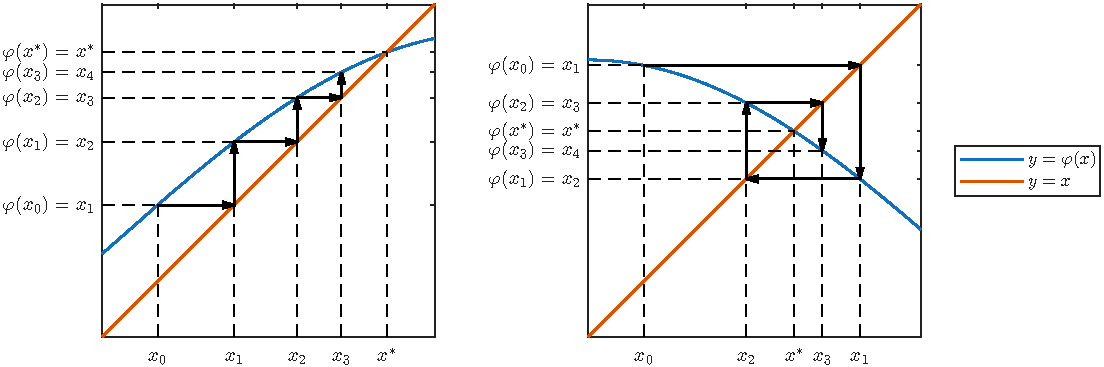
\includegraphics[width=0.95\linewidth]{figures/fixpoint.pdf}
    \captionof{figure}{不动点迭代法示意图}
    \label{fig:fixpoint}
\end{notecaptionblock}

\subsection{迭代法的收敛性}

\begin{theorem}
    {压缩映像原理}{contraction mapping principle}
    若连续函数$\varphi \in \cont[a,b]$满足：
    \begin{itemize}
        \item 像集$\varphi([a,b]) \subset [a,b]$；
        \item Lipschitz条件：$\exists L < 1$，使得$\forall x_1,x_2 \in [a,b]$均有
        \begin{equation}\label{eq:na-contraction-condition}
            \abs{\varphi(x_2) - \varphi(x_1)} \leq L\abs{x_2 - x_1}.
        \end{equation}
    \end{itemize}
    则$\forall x_0 \in [a,b]$，迭代序列$x_{i+1} = \varphi(x_i)$收敛到唯一的不动点$x^*$。且
    \begin{equation}
            \abs{x_k - x^*} \leq \frac1{1 - L}\min\{\abs{x_{k+1} - x_k},L\abs{x_k - x_{k-1}},\ldots,L^k\abs{x_1 - x_0}\}.
    \end{equation}
\end{theorem}

\begin{proof}
    不动点的存在性可由$\psi(x) = \varphi(x) - x$的介值定理可得，唯一性由反证法得到。

    对于不等式，由迭代方程$x_{i+1} = \varphi(x_i)$，可得
    \[
        \abs{x_i - x_{i+1}} = \abs{\varphi(x_{i-1}) - \varphi(x_i)} \leq L\abs{x_{i-1} - x_i},
    \]
    对$x_i - x_{i+p}$进行裂项可得，
    \[
        \abs{x_i - x_{i+p}} \leq \abs{x_i - x_{i+1}} + \cdots + \abs{x_{i+p-1} - x_{i+p}} \leq (1 + L + \cdots + L^{p-1})\abs{x_i - x_{i+1}}.
    \]
    令$p \to \infty$，则$x_{i+p} = x^*$，即得。
\end{proof}

\begin{corollary}
    对于连续函数$\varphi \in \cont^1[a,b]$，将Lipschitz条件换为$\norm{\varphi'}_\infty \leq L < 1$，同样可得$\varphi$在$[a,b]$上存在唯一不动点。
\end{corollary}

\begin{remark}
    \thmref{thm:contraction mapping principle} 给出了$\varphi$在区间$[a,b]$上的全局收敛性。但很多情况下全局收敛性并不容易检验。由此引出$x^*$邻域上的局部收敛性概念。
\end{remark}

\begin{definition}
    {局部收敛性}{local convergence}
    若$x^*$是$\varphi$的不动点，且存在$x^*$的邻域$U$，使得$\forall x^{(0)} \in U$，迭代序列$x^{(k+1)} = \varphi(x^{(k)}) \in U$且$x^{(k)} \to x^*$，则称$x^*$是局部收敛的(local convergence)，$U$为其局部收敛域。
\end{definition}

\begin{corollary}
    若$x^*$为$\varphi$的不动点，$\varphi$在$x^*$某个邻域$U$上连续且$\abs{\varphi'(x^*)} < 1$，则$x^*$局部收敛。
\end{corollary}

\begin{definition}
    {收敛阶}{convergence order}
    给定收敛序列$x_n \to x$，若
    \begin{equation}
        0 < \liminf_{n\to\infty}\frac{\abs{x_{n+1} - x}}{\abs{x_n - x}^p} \leq \limsup_{n\to\infty}\frac{\abs{x_{n+1} - x}}{\abs{x_n - x}^p} < +\infty,
    \end{equation}
    则称序列$x_n$是$p$阶收敛的，
    特别地，$p = 1$称为线性收敛，$p = 2$称为平方收敛；

    若下极限可能为0，则称序列$x_n$是至少$p$阶收敛的；若上极限为0，则称序列$x_n$是超$p$阶收敛的。
\end{definition}

\begin{example}
    {}{}
    \begin{itemize}
        \item 调和序列$\{1/n\}$和等比序列$\{a^n\}~(\abs a < 1)$线性收敛；
        \item 序列$\{\e^{-n^2}\}$超线性收敛，但$\forall\epsilon > 0$都不是超$(1 + \epsilon)$阶收敛；
        \item 序列$\{\e^{-\e^n}\}$是e阶收敛的。
    \end{itemize}
\end{example}

\begin{definition}
    {收敛效率}{}
    若序列$\{x_n\}$通过某种算法收敛于$x$，收敛阶为$p$，计算每个$x_n$的计算量为$\theta$ (不依赖于$n$)，定义
    \begin{equation}\label{eq:na-efficiency-index}
        EI := p^{1/\theta},
    \end{equation}
    表示收敛效率，即单位计算量下算法的收敛率。
\end{definition}

\begin{theorem}
    {单步迭代法的收敛阶}{iteration convergence order}
    设$\varphi$在不动点$x^*$的邻域$U$上属于$\cont^p$。若$p \geq 2$，则对未在有限步到达根的迭代$x_{i+1} = \varphi(x_i)$，
    \begin{center}
        在$x^*$处$p$阶局部收敛$\iff \varphi'(x^*) = \cdots = \varphi^{(p-1)}(x^*) = 0,\enspace\varphi^{(p)}(x^*) \neq 0$
    \end{center}
    对$p = 1$，若$0 < \abs{\varphi'(x^*)} < 1$，则局部线性收敛，渐近误差比为$\abs{\varphi'(x^*)}$。
\end{theorem}

\begin{proof}
    在$x^*$上作Taylor展开，对于$x_k$，$\exists\xi \in U$介于$x_k,x^*$之间使得
    \[
        \varphi(x_k) = \varphi(x^*) + \varphi'(x^*)(x_k - x^*) + \cdots + \frac{\varphi^{(p-1)}(x^*)}{(p - 1)!}(x_k - x^*)^{p-1} + \frac{\varphi^{(p)}(\xi)}{p!}(x_k - x^*)^p,
    \]
    而$\varphi'(x^*) = \cdots = \varphi^{(p-1)}(x^*) = 0$，故
    \[
        \frac{x_{k+1} - x^*}{(x_k - x^*)^p} = \frac{\varphi(x_k) - \varphi(x^*)}{(x_k - x^*)^p}
        = \frac{\varphi^{(p)}(\xi)}{p!} \to \frac{\varphi^{(p)}(x^*)}{p!}.
        \qedhere
    \]
    % 由$\varphi^{(p)}$的连续性即得定理结论。
\end{proof}

\subsection{Newton法}

\begin{theorem}
    {Newton迭代法}{Newton's method}
    若$x_k$是$f(x) = 0$根$x^*$的一个近似，由Taylor展开，
    \[
        f(x^*) = f(x_k) + f'(x_k)(x^* - x_k) + \bigo(x^* - x_k)^2,
    \]
    若$f'(x_k) \neq 0$，由$f(x^*) = 0$，可得
    \[
        x^* = x_k - \frac{f(x_k)}{f'(x_k)} + \bigo(x^* - x_k)^2,
    \]
    忽略二阶项，剩余项作为$x^*$新的近似$x_{k+1}$，可得Newton迭代法：
    \begin{equation}
        \label{eqn:Newton iter}
        x_{k+1} = x_k - \frac{f(x_k)}{f'(x_k)}.
    \end{equation}
\end{theorem}

\begin{corollary}
    对应迭代函数
    \[
        \varphi(x) = x - \frac{f(x)}{f'(x)} \implies \varphi'(x) = \frac{f(x)f''(x)}{f'(x)^2},
    \]
    对简单根$x^*$，若$f$在其附近二阶连续可微，则$\varphi'(x^*) = 0$，从充分近的初值出发可得超线性收敛。
\end{corollary}

\begin{remark}
    Newton法的几何解释：$f$在$x_k$处的切线
    \[
        y = f(x_k) + f'(x_k)(x - x_k),
    \]
    与$x$轴的交点作为$x^*$新的近似$x_{k+1}$。
\end{remark}

\begin{theorem}
    {Newton迭代法的局部收敛性}{convergence of Newton's method}
    若根$x^*$处导数$f'(x^*) \neq 0$且$f''$在$x^*$邻域$U$上连续，则Newton法至少二阶收敛。
\end{theorem}

\begin{proof}
    由Taylor展开，$\exists\xi \in U$介于$x^*,x_k$之间使得
    \[
        f(x^*) = f(x_k) + f'(x_k)(x^* - x_k) + \frac{f''(\xi)}2(x^* - x_k)^2,
    \]
    而$f(x^*) = 0$，故
    \begin{equation}\label{eq:na-newton-quadratic-error}
        \frac{x_{k+1} - x^*}{(x_k - x^*)^2} = \frac{f''(\xi)}{2f'(x_k)} \to \frac{f''(x^*)}{2f'(x^*)}.
    \end{equation}
    故Newton法至少二阶收敛；当$f''(x^*) \neq 0$时，Newton法就是二阶收敛的。
\end{proof}

\begin{remark}
    Newton法至少二阶收敛的前提之一是$f'(x^*) \neq 0$，这相当于说$x^*$是$f$的单重根。
\end{remark}

\begin{definition}
    {$r$重根}{multiple root}
    若
    \begin{equation}\label{eq:na-root-multiplicity}
        f(x^*) = f'(x^*) = \cdots = f^{(r-1)}(x^*) = 0,\enspace f^{(r)}(x^*) \neq 0,
    \end{equation}
    则称$x^*$是$f$的一个$r$重根(multiple root)。
\end{definition}

\begin{corollary}
    若$x^*$是$f$的$r$重根，则$\exists\xi,\eta$介于$x_k,x^*$之间使得，
    \[
        \varphi(x_k) = x_k - \frac{f(x^*) + f'(x^*)(x_k - x^*) + \cdots + f^{(r)}(\xi)(x - x^*)^r/r!}{f'(x^*) + f''(x^*)(x_k - x^*) + \cdots + f^{(r)}(\xi)(x - x^*)^r/(r - 1)!},
    \]
    故
    \[
        \frac{x_{k+1} - x^*}{x_k - x^*} = 1 - \frac1r\frac{f^{(r)}(\xi)}{f^{(r)}(\eta)} \to 1 - \frac1r \geq \frac12.
    \]
    Newton法变为线性收敛的！故需要对Newton法进行改进。
\end{corollary}

\begin{theorem}
    {Newton法的改进}{}
    若$x^*$为$f$的$r$重根，则依前文推论将Newton法\eqref{eqn:Newton iter}改进为二阶收敛的：
    \begin{equation}
        \label{eqn:Newton iter r-multiroot}
        x_{k+1} = x_k - r\frac{f(x_k)}{f'(x_k)},
    \end{equation}
    \tcblower
    对
    \begin{equation}
        u(x) := \frac{f(x)}{f'(x)},
    \end{equation}
    使用Newton法\eqref{eqn:Newton iter}，
    易于验证，$x^*$是$u$的单重根。
\end{theorem}

\subsection{割线法}

下面再介绍一种多步迭代方法。

\begin{theorem}
    {割线法}{secant method}
    以$f$在$x_k,x_{k-1}$的割线斜率(差商)
    \begin{equation}\label{eq:na-secant-slope}
        f[x_k,x_{k-1}] = \frac{f(x_k) - f(x_{k-1})}{x_k - x_{k-1}}
    \end{equation}
    代替Newton法\eqref{eqn:Newton iter}中的导数$f'(x_k)$，称为割线法(secant method)：
    \begin{equation}
        \label{eqn:secant line}
        x_{k+1} = x_k - \frac{x_k - x_{k-1}}{f(x_k) - f(x_{k-1})}f(x_k),
    \end{equation}
\end{theorem}

\begin{theorem}
    {割线法的收敛性}{}
    若在根$x^*$的邻域$U(x^*,\delta) = [x^* - \delta,x^* + \delta]$上$f'(x) \neq 0$且$f \in \cont^2(U)$，若
    \[
        M = \frac{\max_{x\in U}\abs{f''(x)}}{2\min_{x\in U}\abs{f'(x)}} < +\infty,
    \]
    则给定$x_0,x_1 \in U(x^*,\min(\delta,1/M))$，割线法$(1 + \phi)$阶收敛到$x^*$。
\end{theorem}

\begin{proof}
    记$e_k = x_k - x^*$，则
    \[
        e_{k+1} = e_k - \frac{f(x_i) - f(x^*)}{f[x_k,f_{k-1}]} = e_k\frac{f[x_k,x_{k-1}] - f[x_k,x^*]}{f[x_k,x_{k-1}]},
    \]
    故$\exists\xi,\eta \in U$使得
    \[
        e_{k+1} = e_ke_{k-1}\frac{f[x_k,x_{k-1},x^*]}{f[x_k,x_{k-1}]} = e_ke_{k-1}\frac{f''(\xi)}{2f'(\eta)},
    \]
    故
    \[
        \abs{e_{k+1}} \leq \abs{e_k}\abs{e_{k-1}}M \leq \abs{e_k}M\min(\delta,1/M)
    \]
    由于$e_k$至少线性收敛，故 % $\forall\epsilon>0$，$\exists N>0$足够大使得$\forall k>N$，有
    \begin{align*}
        \abs{e_{k+1}} &\approx \abs{e_k}\abs{e_{k-1}}M^*,\\
        M^* &= \frac{\abs{f''(x^*)}}{2\abs{f'(x^*)}},
    \end{align*}
    其中$a_n \approx b_n$表示$a_n - b_n \to 0$（$n \to \infty$）。对上式取对数得到
    \[
        \ln(M^*\abs{e_{k+1}}) \approx \ln(M^*\abs{e_k}) + \ln(M^*\abs{e_{k-1}}),
    \]
    当$k \to \infty$时，上式变为等号，符合Fibonacci数列递推式，故阶数为$1 + \phi = (1 + \sqrt5)/2$。
\end{proof}

\begin{remark}
    Newton法与割线法比较：
    \begin{itemize}
        \item 割线法不用求导；
        \item 当$x_k$接近$x^*$时舍入误差对割线法影响较大；
        \item 割线法的效率$EI_1 = 1 + \phi$；Newton法的效率$EI_2 = 2^{1/\theta}$，其中$\theta$是计算$f'(x)$相对差分的计算量。当
        \[
            \theta > \frac1{\log_2(1 + \phi)} > 1.44
        \]
        时，割线法效率更高。
    \end{itemize}
\end{remark}

\subsection{Aitken加速方法}

由\thmref{thm:iteration convergence order}，若$\abs{\varphi'(x^*)} \in (0,1)$，则迭代收敛速度为线性的。由于
\[
    x_{k+2} - x^* = \varphi'(\xi)(x_{k+1} - x^*) \approx \varphi'(x^*)(x_{k+1} - x^*),
\]
下一项$x_{k+1} - x^* \approx \varphi'(x^*)(x_k - x^*)$，故可联立消掉$\varphi'(x^*)$，得到：
\[
    x^* \approx x_k - \frac{(x_{k+1} - x_k)^2}{x_{k+2} - 2x_{k+1} + x_k} \equiv x_k - \frac{\Delta x_k^2}{\Delta^2 x_k}.
\]
其中差分$\Delta x_k = x_{k+1} - x_k$，二阶差分$\Delta^2x_k = \Delta x_{k+1} - \Delta x_k$。和微分记号一样，约定$\Delta x_k^2 \equiv (\Delta x_k)^2$，而$\Delta(x_k^2)$需要加括号。

\begin{theorem}
    {Aitken加速方法}{Aitken}
    若$x_k$至少线性收敛到$x^*$，则可定义
    \begin{equation}
        \label{eqn:Aitken}
        x_k' := x_k - \frac{\Delta x_k^2}{\Delta^2x_k},
    \end{equation}
    并且$x_k'$收敛比$x_k$快：
    \begin{equation}\label{eq:na-aitken-acceleration}
        \lim_{k\to\infty}\frac{x_k' - x^*}{x_k - x^*} = 0.
    \end{equation}
\end{theorem}

\begin{proof}
    记$e_k := x_k - x^*$，由$x_k$至少线性收敛，$\exists\lambda$且$\abs\lambda < 1$使得
    \[
        e_{k+1} = (\lambda + \delta_k)e_k,\quad\delta_k \to 0.
    \]
    则
    \begin{align*}
        \Delta x_k &= e_{k+1} - e_k = e_k[(\lambda - 1) + \delta_k],\\
        \Delta^2x_k &= e_{k+2} - 2e_{k+1} + e_k = e_k[(\lambda + \delta_{k+1})(\lambda + \delta_k) - 2(\lambda + \delta_k) + 1] = e_k[(\lambda - 1)^2 + \mu_k],
    \end{align*}
    其中$\mu_k = \lambda(\delta_{k+1} + \delta_k) - 2\delta_k + \delta_k\delta_{k+1} \to 0$。当$k$充分大时，$\Delta^2x_k \neq 0$，可定义$x_k'$，且
    \[
        \lim_{k\to\infty}\frac{x_k' - x^*}{x_k - x^*} = \lim_{k\to\infty}1 - \frac{[(\lambda - 1) + \delta_k]^2}{(\lambda - 1)^2 + \mu_k} = 0.
        \qedhere
    \]
\end{proof}

\begin{remark}
    Aitken加速方法只需给定序列$x_k$，其公式\eqref{eqn:Aitken}与序列$x_k$的产生方法$\varphi$无关。
\end{remark}

\Needspace{10\baselineskip}
\subsection{Steffensen迭代法}

\begin{theorem}
    {Steffensen迭代法}{Steffensen}
    对Aitken加速公式\eqref{eqn:Aitken}利用$x_{k+1} = \varphi(x_k),\,x_{k+2} = \varphi(\varphi(x_k))$作为新的迭代公式：
    \begin{equation}\label{eq:na-steffensen-iteration}
        \hat x_{k+1} = \hat x_k - \frac{(\varphi(\hat x_k) - \hat x_k)^2}{\varphi(\varphi(\hat x_k)) - 2\varphi(\hat x_k) + \hat x_k}.
    \end{equation}
    这实际上根据$\varphi$定义了新的迭代函数
    \begin{equation}
        \psi(x) = x - \frac{(\varphi(x) - x)^2}{\varphi(\varphi(x)) - 2\varphi(x) + x} = \frac{x\varphi(\varphi(x)) - \varphi(x)^2}{\varphi(\varphi(x)) - 2\varphi(x) + x}.
    \end{equation}
    若$x^*$是$\psi$的不动点，则$x^*$也是$\varphi$的不动点；

    若$x^*$是$\varphi$的不动点，$\varphi \in \cont^1(U)$且$\varphi'(x^*) \neq 1$，则$x^*$是$\psi$的不动点。
\end{theorem}

\begin{proof}
    由$\psi$表达式可得，
    % \[
    %     (x-\psi(x))(\varphi(\varphi(x))-2\varphi(x)+x)=(\varphi(x)-x)^2,
    % \]
    $\psi(x^*) = x^* \implies \varphi(x^*) = x^*$；
    而$\varphi(x^*) = x^*$时，$\psi(x^*)$出现0/0型，由L'H\^opital法则
    \[
        \psi(x^*) = x^* - \lim_{x\to x^*}\frac{(\varphi(x) - x)^2}{\varphi(\varphi(x)) - 2\varphi(x) + x} = x^* - \frac{2(\varphi(x^*) - x^*)(\varphi'(x^*) - 1)}{\varphi'(\varphi(x^*))\varphi'(x^*) - 2\varphi'(x^*) + 1} = x^*.
        % \frac{\varphi(\varphi(x^*))+x^*\varphi'(\varphi(x^*))\varphi'(x^*)-2\varphi(x^*)\varphi'(x^*)}{\varphi'(\varphi(x^*))\varphi'(x^*)-2\varphi'(x^*)+1}=x^*.
        \qedhere
    \]
\end{proof}

\begin{remark}
    证明中分母出现了$\varphi'(x^*) - 1$，故要求$\varphi'(x_k) \neq 1$，即$x^*$不是$\varphi(x) - x = 0$的重根。
    但事实上$\varphi'(x^*) = 1$也可以证明$\psi(x^*) = x^*$。
\end{remark}

\begin{theorem}
    {Steffensen迭代法的收敛阶}{convergence order Steffensen}
    若$x_{k+1} = \varphi(x_k)$是$p$阶收敛的($p > 1)$，则$x_{k+1} = \psi(x_k)$是$(2p - 1)$阶收敛的。

    若$p = 1$且$\varphi'(x^*) \neq 1$，则$x_{k+1} = \psi(x_k)$是二阶收敛的。
\end{theorem}

\begin{proof}
    由$\varphi$是$p$阶收敛的：$\varphi(x) - x^* = \Theta(x - x^*)^p,\;\varphi(\varphi(x)) - x^* = \Theta(x - x^*)^{2p}$，
    \begin{align*}
        \psi(x) - x^* &= \frac{(x - x^*)(\varphi(\varphi(x)) - x^*) - (\varphi(x) - x^*)^2}{\varphi(\varphi(x)) - x^* - 2(\varphi(x) - x^*) + x - x^*}\\
        &= \frac{\Theta(x - x^*)^{2p+1} - \Theta(x - x^*)^{2p}}{\Theta(x - x^*)^{2p} - \Theta(x - x^*)^p + x - x^*} = \Theta(x - x^*)^{2p-1}.
        \qedhere
    \end{align*}
\end{proof}

\begin{remark}
    若$\varphi \in \cont^2(U)$且$\varphi'(x^*) \neq 1$，则Steffensen法不但可以提高收敛速度(至少二阶收敛)，在$\abs{\varphi'(x^*)} > 1$时还可以把不收敛的方法改进为二阶收敛的方法。
    但当$p > 1$时，Steffensen法一般好处不大，故其多用于改进线性收敛的情形。
\end{remark}

\begin{example}
    {}{}
    特别地，$\varphi(x) = x + f(x)$，
    % 则$\varphi(\varphi(x))=\varphi(x+f(x))=x+f(x)+f(x+f(x))$
    可得
    \begin{equation}
        \psi(x) = x - \frac{f(x)^2}{f(x + f(x)) - f(x)}.
    \end{equation}
    若$f(x^*) = 0$，可得$\psi(x^*) = x^*,\;\psi'(x^*) = 0$故$x_{k+1} = \psi(x_k)$至少二阶收敛。
\end{example}

\section{非线性方程组的不动点迭代法}

\begin{definition}
    {向量值函数}{vector function}
    向量值函数是一个映射$F:D \to \RR^n$，其中$D \subset \RR^n$，其分量是多元标量函数$f_i:D \to \RR$：
    \begin{equation}
        F(x) = \begin{bmatrix}
            f_1(x_1,\ldots,x_n)\\\vdots\\f_m(x_1,\ldots,x_n)
        \end{bmatrix}
    \end{equation}
\end{definition}

\begin{definition}
    {向量值函数的连续性}{vector function continuous}
    给定点$x_0 \in D$，若$\forall\epsilon > 0,\;\exists\delta > 0$使得领域内$\forall x \in B(x_0,\delta) \subset D$均有
    \[
        \norm{F(x) - F(x_0)} < \epsilon,
    \]
    则称$F$在$x_0$处连续。
\end{definition}

\begin{definition}
    {向量值函数的导数}{}
    给定$x \in D$和充分小$h$使得$x + h \in D$，若存在矩阵$A(x) \in \RR^{m\times n}$满足
    \begin{equation}
        \lim_{h\to 0}\frac{\norm{F(x + h) - F(x) - A(x)h}}{\norm h} = 0,
    \end{equation}
    则称$F$在$x$处可微，$A(x) =: F'(x)$称为$F$的导数，事实上就是Jacobi矩阵：
    \begin{equation}
        F'(x) = \begin{bmatrix}
            \pv{f_1}{x_1}&\cdots&\pv{f_1}{x_n}\\
            \vdots&\ddots&\vdots\\
            \pv{f_m}{x_1}&\cdots&\pv{f_m}{x_n}
        \end{bmatrix}
    \end{equation}
\end{definition}

\begin{theorem}
    {压缩映像原理(向量形式)}{contraction mapping principle (vector)}
    连续函数$\varphi:D \subset \RR^n \to \RR^n$满足：
    \begin{itemize}
        \item 闭性：$D$是闭集；
        \item 映内性：$\varphi(D) \subset D$；
        \item 压缩性：$\exists L < 1$，使得$\forall x_1,x_2 \in D$，
        \begin{equation}\label{eq:na-vector-contraction}
            \norm{\varphi(x_2) - \varphi(x_1)} \leq L\norm{x_2 - x_1},
        \end{equation}
    \end{itemize}
    则$\forall x_0 \in D$，迭代序列$x_{k+1} = \varphi(x_k)$收敛到$\varphi$唯一的不动点$x^*$。
\end{theorem}

\begin{remark}
    压缩性依赖于范数的选择。如$\varphi(x) = Ax$，其中
    \[
        \varphi'(x) = A = \begin{bmatrix}
            0.1&0.9\\0&0.1
        \end{bmatrix}.
    \]
    在2-范数下$\norm A_2 < 1$可压缩，但在无穷范数下$\norm A_\infty = 1$不可压缩。
\end{remark}

\begin{definition}
    {局部收敛性(向量形式)}{}
    给定$\varphi(x^*)$的不动点，若存在$x^*$的一个邻域$S \subset D$使得$\forall x^{(0)} \in S$，$x^{(k+1)} = \varphi(x^{(k)}) \in S$且$x^{(k)} \to x^*$，则称$x^*$是局部收敛的。
\end{definition}

\begin{theorem}
    {}{}
    若$\exists L \in (0,1)$和某个范数$\norm \cdot$使得$\forall x \in S(x^*,\delta)$均有
    \[
        \norm{\varphi(x) - \varphi(x^*)} \leq L\norm{x - x^*},
    \]
    则$x^*$是局部收敛的。
\end{theorem}

\begin{corollary}
    一个充分条件：若存在一个算子范数使得$\norm{\varphi'(x^*)} < 1$，则$x^*$是局部收敛的。
\end{corollary}

\begin{theorem}
    {Newton法(向量形式)}{}
    给定$x^{(0)}$，计算 
    \begin{equation}\label{eq:na-multivariate-newton}
        x^{(k+1)} = x^{(k)} - F'(x^{(k)})\inv F(x^{(k)}).
    \end{equation}
\end{theorem}

\begin{remark}
    Newton法的一个显著缺点是需要反复计算$F'$。可借鉴割线法改进。
\end{remark}

\begin{theorem}
    {修正的Newton法}{}
    将Jacobi矩阵$F'(x^{(k)})$替换为矩阵$A^{(k)}$：
    \begin{equation}\label{eq:na-quasi-newton}
        x^{(k+1)} = x^{(k)} - {A^{(k)}}\inv F(x^{(k)}),
    \end{equation}
    矩阵$A^{(k)}$满足拟Newton方程：
    \begin{equation}
        A^{(k)}(x^{(k)} - x^{(k-1)}) = F(x^{(k)}) - F(x^{(k-1)}),
    \end{equation}
    显然$A^{(k)}$的取法并不唯一，可以迭代地写成
    \[
        A^{(k+1)} = A^{(k)} + \Delta A^{(k)},
    \]
    且$\rank(A^{(k)})$一般为1或2，即$A^{(k+1)}$是$A^{(k)}$的一个低秩修正。
\end{theorem}

\begin{theorem}
    {Broyden秩1方法}{}
    令$p^{(k)} = x^{(k+1)} - x^{(k)},\;q^{(k)} = F(x^{(k+1)}) - F(x^{(k)})$，设$\Delta A^{(k)} = u^{(k)}{v^{(k)}}\transp$是秩1矩阵，则
    \[
        (A^{(k)} + u^{(k)}{v^{(k)}}\transp)p^{(k)} = q^{(k)} \implies u^{(k)} = \frac{q^{(k)} - A^{(k)}p^{(k)}}{{v^{(k)}}\transp p^{(k)}},
    \]
    可令$v^{(k)} = p^{(k)}$，则
    \begin{subequations}
        \begin{align}
            x^{(k+1)} &= x^{(k)} - {A^{(k)}}\inv F(x^{(k)}),\\
            \Delta A^{(k)} &= \frac{(q^{(k)} - A^{(k)}p^{(k)}){p^{(k)}}\transp}{\norm{p^{(k)}}^2},\\
            A^{(k+1)} &= A^{(k)} + \Delta A^{(k)}.
        \end{align}
    \end{subequations}
\end{theorem}

\chapter{矩阵特征值}
\label{chap:eigenvalue}

\begin{definition}
    {矩阵特征值问题}{}
    给定$n\times n$矩阵$A$，寻找$\lambda\in\CC$和非零向量$x\in\CC^n$，使得
    \begin{equation}
        Ax=\lambda x,
    \end{equation}
    $\lambda$称为$A$的特征值(eigenvalue)，$x$称为对应的特征向量(eigenvector)。
\end{definition}

\begin{corollary}
    矩阵特征值满足特征多项式方程
    \begin{equation}
        \det(\lambda I-A)=0.
    \end{equation}
\end{corollary}

\paragraph{特征值的分布估计}

由式\eqref{eqn:rho<=norm} $\sigma(A)\leq\norm A$可知，在复平面上，$A$的特征值都位于以原点为中心、(某一)矩阵范数$\norm A$为半径的圆盘内。
当然，这种对特征值界限的估计过于粗糙。

\begin{theorem}
    {Gershgorin圆盘定理·一}{Gershgorin circle theorem I}
    定义$A$的第$i$行Gershgorin圆盘为
    \begin{equation}
        D_i:=\set{z\in\CC}{\abs{z-a_{ii}}\leq r_i},\quad r_i:=\sum_{j\neq i}\abs{a_{ij}}.
    \end{equation}
    则$A$的所有特征值都位于这些圆盘的并集中，即
    \begin{equation}
        \lambda\in\bigcup_{i=1}^nD_i.
    \end{equation}
\end{theorem}

\begin{proof}
    设$\lambda$为$A$的特征值，$x$为对应的特征向量。
    令$k=\argmax_i\abs{x_i}$，则
    \[
        \abs{\lambda - a_{kk}}\abs{x_k}=\biggabs{\sum_{j\neq k}a_{kj}x_j}\leq\sum_{j\neq k}\abs{a_{kj}}\abs{x_j}\leq r_k\abs{x_k}.
    \]
    故$\abs{\lambda - a_{kk}}\leq r_k$，即$\lambda\in D_k$。
\end{proof}

\begin{theorem}
    {Gershgorin圆盘定理·二}{Gershgorin circle theorem II}
    如果$k$个Gershgorin圆盘$D_{i_1},\ldots,D_{i_k}$与其他圆盘互不相交，则它们的并集中恰有$k$个特征值。
\end{theorem}

\begin{proof}
    将$A=L+D+U$分解为严格下三角矩阵$L$、对角矩阵$D$和严格上三角矩阵$U$之和。定义
    \[
        A(\theta):=D+\theta(L+U),\quad\theta\in[0,1].
    \]
    显然$A(1)=A,\,A(0)=D$。
    易得$A(\theta)$的Gershgorin圆盘为
    \[
        D_i(\theta)=\set{z\in\CC}{\abs{z-a_{ii}}\leq \theta r_i},
    \]
    因此$D_i(\theta)\subseteq D_i(1)=D_i$。
    由于$D_{i_1},\ldots,D_{i_k}$与其他圆盘互不相交，故$D_{i_1}(\theta),\ldots,D_{i_k}(\theta)$也与其他圆盘互不相交。

    易得$A(\theta)$的特征多项式关于$\theta$连续变化，故其特征值也关于$\theta$连续变化。
    注意到$D_i(0)$退化为单点$\{a_{ii}\}$，每个$D_i(0)$中都恰有一个特征值。
    考虑$\theta$从0变化到1的过程，由于$D_{i_1}(\theta),\ldots,D_{i_k}(\theta)$与其他圆盘互不相交，其并集中始终有$k$个特征值。
\end{proof}

\begin{center}
    \tikzfigure{gershgorin-disks}
    \captionof{figure}{Gershgorin圆盘定理}
    \label{fig:Gershgorin circle theorem}
\end{center}

\begin{corollary}
    为了更好的估计，可以设法缩小一些Gershgorin圆盘的半径。
    例如$A$与其相似变换$BAB\inv$有相同的特征值，若$B=\diag(b_1,\ldots,b_n)$，则Gershgorin圆盘的半径变为
    \[
        r_i'=\sum_{j\neq i}\biggabs{\frac{b_j}{b_i}a_{ij}}.
    \]
\end{corollary}

\begin{example}
    {}{}
    考虑矩阵$A$及其相似变换$BAB\inv$
    \[
        A=\begin{bmatrix}
            0.9&0.01&0.12\\
            0.01&0.8&0.13\\
            0.01&0.02&0.4
        \end{bmatrix},\quad
        BAB\inv=\begin{bmatrix}
            0.9&0.01&0.012\\
            0.01&0.8&0.013\\
            0.1&0.2&0.4
        \end{bmatrix},
    \]
    其中选取了$B=\diag(1,1,0.1)$，原先$A$的$D_1,D_2$有较大重叠而$D_3$半径较小且孤立，变换后$D_1',D_2'$半径大幅缩小，从而更好地分离了三个圆盘。
\end{example}



\chapter{函数插值和重构}
\label{chap:interpolation}

\paragraph{基本问题}
已知关于某函数$f$的一组信息，如何重构$f$？事实上，由于信息缺失，无法准确重构。

\begin{definition}
    {重构}{}
    给定函数空间$X$上的一组线性无关泛函$\phi_1,\ldots,\phi_n$，$f\in X$且$\phi_i(f)$已知，希望确定$f^*\in Y\subset X$满足：
    \begin{equation}
        \phi_i(f^*)=\phi_i(f),\quad i=1,\ldots,n.
    \end{equation}
    $Y$称为插值空间或重构空间，$\{\phi_i\}$为信息泛函。
\end{definition}

% \begin{remark}
%     几个基本问题：
%     \begin{itemize}
%         \item 存在性和唯一性；
%         \item 算法；
%         \item 合理性。
%     \end{itemize}
% \end{remark}

\begin{example}
    {采样空间的选择}{}
    \begin{itemize}
        \item 多项式函数空间
        \[
            \poly_n=\{a_0+a_1x+\cdots+a_nx^n\},
        \]
        \item 样条函数(spline)空间：分段多项式函数；
        \item 三角多项式函数空间
        \[
            \mathcal Y_n=\{a_0+a_1\cos x+b_1\sin x+\cdots+a_n\cos nx+b_n\sin nx\}.
        \]
    \end{itemize}
\end{example}

\section{一维多项式插值}
\label{sec:1-D polynomial interpolation}

\subsection{Lagrange插值}

\begin{definition}
    {Lagrange插值}{Lagrange interpolation}
    插值空间$Y$由$n+1$个参数$a_0,\ldots,a_n$标定，即
    \[
        y=y(x;a_0,\ldots,a_n).
    \]
    给定一组插值节点(采样点) $x_i$和采样值$f_i=f(x_i)$，希望确定参数满足
    \begin{equation}
        y(x_i)=f(x_i),\quad\forall i\in I.
    \end{equation}
\end{definition}

\begin{theorem}
    {多项式插值定理}{}
    给定$n+1$个不同插值点$x_0,\ldots,x_n$，存在唯一的多项式函数$p_n\in\poly_n$满足插值条件。
\end{theorem}
\begin{proof}
    存在性：
    采取直接构造的方法。
    定义插值基函数$\ell_i\in\poly_n$：
    \begin{equation}
        \label{eqn:Lagrange base}
        \ell_i(x):=\prod_{j\neq i}\frac{x-x_j}{x_i-x_j}.
    \end{equation}
    易验证，$\ell_i$满足：
    \begin{equation}
        \ell_i(x_j)=\delta_{ij}.
    \end{equation}
    故插值多项式为
    \begin{equation}
        \label{eqn:Lagrange polynomial}
        p_n(x)=\sum_{i=0}^nf(x_i)\ell_i(x).
    \end{equation}
    唯一性：
    若还存在$q_n\in\poly_n$满足插值条件，则$p_n-q_n\in\poly_n$且有$x_0,\ldots,x_n$共$n+1$个零点，故$p_n-q_n\equiv 0$。
\end{proof}

\begin{definition}
    {余项}{remainder}
    定义插值函数$p_n(x)$与被插值函数$f(x)$之间的差为余项(remainder)
    \begin{equation}
        R_n(x):=f(x)-p_n(x).
    \end{equation}
\end{definition}

\begin{theorem}
    {中值定理与余项}{mean value theorem of remainder}
    若$f\in\cont^{n+1}[a,b]$，则$\forall x\in[a,b],\exists\xi(x)\in(a,b)$使得
    \begin{equation}
        \label{eqn:Lagrange remainder}
        R_n(x)=\frac{f^{(n+1)}(\xi(x))}{(n+1)!}\prod_{i=0}^n(x-x_i).
    \end{equation}
\end{theorem}

\begin{proof}
    当$x=x_i$时，$R_n(x_i)=0$显然成立；
    给定$x\in[a,b]$且$x\neq x_i$，定义
    \[
        g(t):=R_n(t)-\frac{\prod_{i=0}^n(t-x_i)}{\prod_{i=0}^n(x-x_i)}R_n(x),
    \]
    则$g\in\cont^{n+1}[a,b]$且在$[a,b]$上有$x_0,\ldots,x_n,x$共$n+2$个零点，在其划分的$n+1$个区间中应用Rolle定理：对应存在$\xi_1^{(1)},\ldots,\xi_{n+1}^{(1)}$使得
    \[
        g'(\xi_i^{(1)})=0,\quad i=0,1,\ldots,n+1,
    \]
    继续对$\xi_0^{(1)},\ldots,\xi_{n+1}^{(1)}$划分的$n$个区间上应用Rolle定理，直到$g^{(n+1)}(\xi^{(n+1)}_0)=0$：
    \[
        g^{(n+1)}(\xi^{(n+1)}_0)=f^{(n+1)}(\xi^{(n+1)}_0)-\frac{(n+1)!}{\prod_{i=0}^n(x-x_i)}R_n(x)=0.
    \]
    取$\xi=\xi_0^{(n+1)}$即证。
\end{proof}

\begin{corollary}
    若$f\in\cont^{n+1}[a,b]$，$h=\max(x_{i+1}-x_i)$则
    \begin{equation}
        \norm{R_n}_\infty\leq\frac{h^{n+1}}{4(n+1)}\norm{f^{(n+1)}}_\infty.
    \end{equation}
\end{corollary}

\subsection{Lagrange插值的收敛性}

当什么条件下，$n\to\infty$，误差$\norm{R_n}_\infty\to 0$？

\begin{theorem}
    {Lagrange插值收敛性的一个充分条件}{}
    若被插值函数的任意阶导数一致有界，则误差收敛到0。
\end{theorem}

\begin{example}
    {}{}
    给定$f(x)=\sin x,\enspace x\in[0,\pi]$，由于$\forall x\in[0,\pi]$
    \[
        \abs{f^{(n+1)}(x)}\leq 1,\quad\abs{\prod_{i=0}^n(x-x_i)}\leq\pi^{n+1},
    \]
    故
    \[
        \abs{R_n(x)}\leq\frac{\pi^{n+1}}{(n+1)!}\to0,
    \]
    说明Lagrange插值多项式$p_n$在$[0,\pi]$上一致收敛到$f$。
\end{example}

% \begin{theorem}
%     {误差收敛性的一个充分条件}{}
%     记$\delta:=\abs{I(x_0,\ldots,x_n)}$，$\tilde x$为$I$的中心。如果$f$在$B(\tilde x,2\delta)$上复解析，则插值法在$I$上是收敛的。
% \end{theorem}

% \begin{proof}
%     设$M$为$f$在$\Omega=B(\tilde x,1.9\delta)$上的上界，则
%     \begin{equation}
%         \frac{f^{n+1}(\xi)}{(n+1)!}=\frac1{2\pi\i}\oint_{\p\Omega}\frac{f(z)}{(z-\xi)^{n+2}}\d z,
%     \end{equation}
%     于是
%     \begin{equation*}
%         \abs{R_n(x)}\leq C\delta\frac{\delta^{n+1}}{(1.4\delta)^{n+2}}\to 0.
%         \qedhere
%     \end{equation*}
% \end{proof}

\begin{example}
    {Runge现象}{Runge's phenomenon}
    Runge函数$f(x)=\frac1{1+25x^2}$在$[-1,1]$上等距插值。
    \begin{center}
        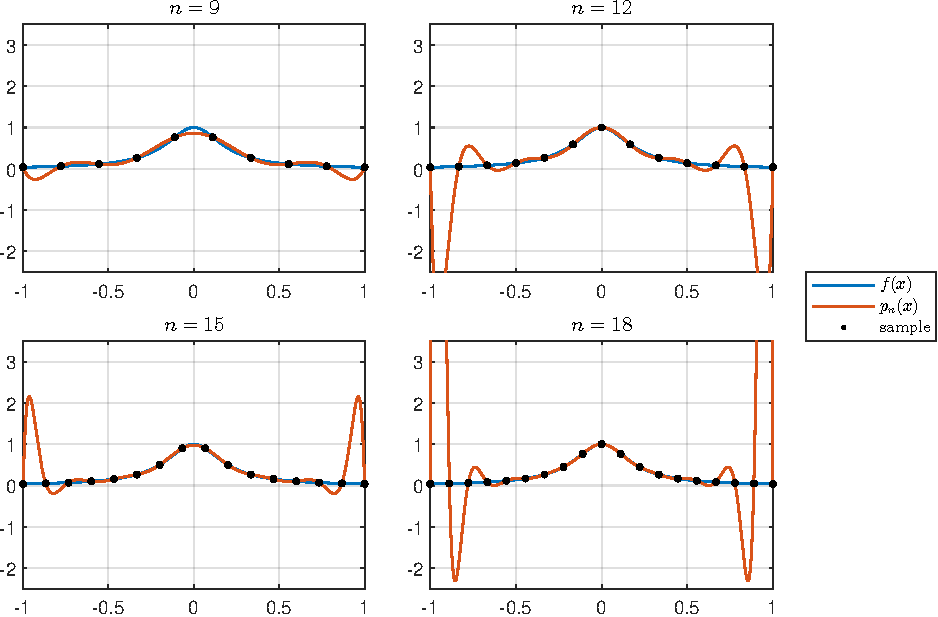
\includegraphics[width=0.9\linewidth]{figures/Runge.pdf}
        \captionof{figure}{等距插值Runge现象}
    \end{center}
    显然$f(x)$在$\RR$上是解析的，但在$\CC$上存在奇点$\pm\i/5$。
    \tcblower
    改用$n+1$阶Chebyshev多项式零点
    \[
        \cos\biggp{\frac{\pi}{2(n+1)}},\enspace
        \cos\biggp{\frac{3\pi}{2(n+1)}},\enspace
        \ldots,\enspace
        \cos\biggp{\frac{2n+1}{2(n+1)}\pi},
    \]
    作为插值节点，可以消去Runge现象。
    \begin{center}
        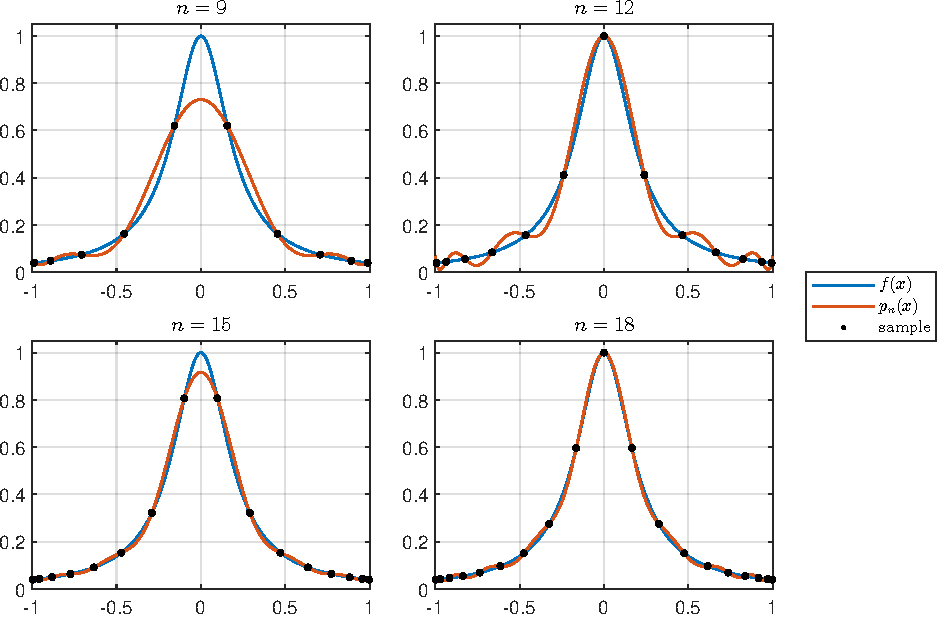
\includegraphics[width=0.9\linewidth]{figures/Rungeless.pdf}
        \captionof{figure}{Chebyshev多项式零点插值}
    \end{center}
\end{example}

\subsection{Newton插值公式}

\iffalse
\begin{table}[h]
    \centering
    \begin{tabular}{cccc}
        \toprule
        0&1&2&3\\
        \midrule 
        \begin{tabular}[c]{@{}c@{}}
            $P_0$\\$P_1$\\$P_2$\\$P_3$
        \end{tabular} & 
        \begin{tabular}[c]{@{}c@{}}
            $P_{01}$\\$P_{12}$\\$P_{23}$
        \end{tabular} & 
        \begin{tabular}[c]{@{}c@{}}
            $P_{012}$\\$P_{123}$
        \end{tabular} & $P_{0123}$ \\
        \bottomrule
    \end{tabular}
\end{table}
\fi

\begin{definition}
    {均差}{divided differences}
    定义$f$在节点集$i_0,i_1,\ldots,i_k$上的$k$阶均差(divided differences)递归地定义为：
    \begin{equation}
        f[x_{i_0},\ldots,x_{i_k}]:=\frac{f[x_{i_1},\ldots,x_{i_k}]-f[x_{i_0},\ldots,x_{i_{k-1}}]}{x_{i_k}-x_{i_0}}.
    \end{equation}
    特别地，$f$在$x_i$上的零阶均差$f[x_i]:=f(x_i)$。
\end{definition}

\begin{corollary}
    $k$阶均差$f[x_0,\ldots,x_k]$是$f(x_0),\ldots,f(x_k)$的线性组合：
    \begin{equation}
        f[x_0,\ldots,x_k]=\sum_{i=0}^k\frac{f(x_i)}{\prod_{j\neq i}(x_i-x_j)}.
    \end{equation}
    因此，均差对于节点是对称的，即任意改变节点的顺序，均差的值不变。
\end{corollary}

% 如果$f$足够光滑，则
% \begin{equation}
%     \lim_{\epsilon_i\to0}f[x_0^{\epsilon_0},\ldots,x_n^{\epsilon_n}]=f[x_0,\ldots,x_n],
% \end{equation}

\begin{theorem}
    {Newton插值公式}{}
    利用均差迭代得到$n$次Newton插值多项式：
    \begin{equation}
        p_n(x)=f(x_0)+f[x_0,x_1](x-x_0)+\cdots+f[x_0,\ldots,x_n](x-x_0)\cdots(x-x_{n-1}).
    \end{equation}
    其余项为
    \begin{equation}
        R_n(x)=f[x,x_0,\ldots,x_n](x-x_0)\cdots(x-x_n).
    \end{equation}
    % \begin{equation}
    %     \begin{aligned}
    %         P_{i_0\cdots i_k}(x)&=P_{i_0\cdots i_{k-1}}(x)+f[x_{i_0},\ldots,x_{i_k}](x-x_{i_0})\cdots(x-x_{i_{k-1}})\\
    %         &=f[x_{i_0}]+f[x_{i_0},x_{i_1}](x-x_{i_0})+\cdots\\
    %         &\qqquad~+f[x_{i_0},\ldots,x_{i_k}](x-x_{i_0})\cdots(x-x_{i_{k-1}}).
    %     \end{aligned}
    % \end{equation}
\end{theorem}

对均差形式的余项应用\thmref{thm:mean value theorem of remainder} 得到：

\begin{theorem}
    {中值定理与均差}{mean value theorem of divided differences}
    如果$f\in\cont[a,b],\enspace x_0,\ldots,x_n\in[a,b]$，则$\exists\xi\in I(x_0,\ldots,x_n)$，
    \begin{equation}
        f[x_0,\ldots,x_n]=\frac{f^{(n)}(\xi)}{n!}.
    \end{equation}
\end{theorem}

\begin{corollary}
    特别地，$n$阶均差：
    \begin{equation}
        f[\underbrace{x,\ldots,x}_{n+1}]=\frac{f^{(n)}(x)}{n!}
    \end{equation}
\end{corollary}
\begin{corollary}
    均差的导数：
    \begin{equation}
        \dd xf[x_0,\ldots,x_n,x]=f[x_0,\ldots,x_n,x,x].
    \end{equation}
\end{corollary}

\begin{theorem}
    {Neville算法}{Neville's algorithm}
    给定插值节点$x_0,\ldots,x_n$，定义$p_{i,j}\in\poly^{j-i}$为满足节点$x_i,\ldots,x_j$插值条件的多项式插值函数，则递归地，有$p_{i,i}(x)\equiv f(x_i)$，
    \begin{equation}
        \label{eqn:Neville}
        p_{i,j}(x)=\frac{(x-x_i)p_{i+1,j}(x)+(x_j-x)p_{i,j-1}(x)}{x_j-x_i},
    \end{equation}
\end{theorem}

\subsection{Hermite插值}

现推广Lagrange插值的概念：除了要求插值函数在节点上相等外，还要求在节点上的导数值相等。

\begin{definition}
    {Hermite插值问题}{}
    给定插值节点$x_0<x_1<\cdots<x_m$及插值条件
    \[
        (x_i,f^{(k)}(x_i)),\enspace i=0,1,\ldots,m,\enspace k=0,1,\ldots,n_i-1
    \]
    确定次数为$n=n_0+\cdots+n_m-1$的多项式函数$p\in\poly_n$满足插值条件。
    % \begin{equation}
    %     P^{(k)}(\xi_i)=f_i^{(k)},\quad i=0,1,\ldots,m,\enspace k=0,1,\ldots,n_i-1.
    % \end{equation}
\end{definition}

\begin{theorem}
    {}{}
    Hermite插值问题的解存在且唯一。
\end{theorem}

\begin{proof}
    定义拓展均差：
    \begin{equation}
        \begin{aligned}
            f[x_0,x_1,\ldots,x_n]:={}&\int_0^{t_0}\int_0^{t_1}\cdots\int_0^{t_{n-1}}\\
            &f^{(n)}(t_n(x_n-x_{n-1})+\cdots+t_1(x_1-x_0)+t_0x_0)\d t_n\cdots\nd t_2\nd t_1.
        \end{aligned}
    \end{equation}
    有递推式：
    \begin{equation}
        f[x_0,\ldots,x_n]=\frac{f[x_0,\ldots,x_{n-2},x_n]-f[x_0,\ldots,x_{n-1}]}{x_n-x_{n-1}}.
    \end{equation}
    即证。
\end{proof}


\begin{example}
    {均差表}{divided difference table}
    给定$f(a),f'(a),f(b),f'(b)$，则插值函数
    \[
        p_3(x)=f(a)+f[a,a](x-a)+f[a,a,b](x-a)^2+f[a,a,b,b](x-a)^2(x-b).
    \]
    计算到$f[a,a,b,b]$，给出均差表：
    \begin{center}
        \begin{tabular}{cccc}
            \toprule
            0&1&2&3\\
            \midrule 
            \begin{tabular}[c]{@{}c@{}}
                $f(a)$\\$f(a)$\\$f(b)$\\$f(b)$
            \end{tabular} & 
            \begin{tabular}[c]{@{}l@{}}
                $f[a,a]=f'(a)$\\[.5ex]$f[a,b]=\frac{f(b)-f(a)}{b-a}$\\$f[b,b]=f'(b)$
            \end{tabular} & 
            \begin{tabular}[c]{@{}c@{}}
                $f[a,a,b]=\frac{f[a,b]-f[a,a]}{b-a}$\\[1ex]
                $f[a,b,b]=\frac{f[b,b]-f[a,b]}{b-a}$
            \end{tabular} & $f[a,a,b,b]=\cdots$ \\
            \bottomrule
        \end{tabular}
    \end{center}
\end{example}

% \begin{theorem}
%     {Hermite插值问题的Newton公式}{}
%     插值多项式为
%     \begin{equation}
%         P(x)=f[x_0]+f[x_0,x_1](x-x_0)+\cdots+f[x_0,\ldots,x_n](x-x_0)\cdots(x-x_{n-1}).
%     \end{equation}
%     其中$x_0,\ldots,x_n$是以下序列的任意置换
%     \[
%         \underbrace{\xi_0,\ldots,\xi_0}_{n_0},\ldots,\underbrace{\xi_m,\ldots,\xi_m}_{n_m}.
%     \]
% \end{theorem}




\section{分段插值}
\label{sec:piecewise interpolation}

\subsection{分段线性插值}

\begin{definition}
    {分段线性插值}{}
    给定节点$a=x_0<x_1<\cdots<x_n=b$及$f(x_i)$，求插值函数$\varphi$满足：
    \begin{itemize}
        \item $\varphi\in\cont[a,b]$是连续函数；
        \item $[x_i,x_{i+1}]$上$\varphi\in\poly_1$是线性函数；
        \item $\varphi(x_i)=f(x_i)$。
    \end{itemize}
    满足前两个性质的函数组成插值空间$\Phi$，且$\dim(\Phi)=n+1$。
\end{definition}

\begin{theorem}
    {}{}
    分段线性插值函数是存在且唯一的。
\end{theorem}

\begin{proof}
    定义插值基函数
    \begin{equation}
        I_i(x)=\begin{cases}
            \frac{x-x_{i-1}}{x_i-x_{i-1}},&x\in[x_{i-1},x_i]\\
            \frac{x_{i+1}-x}{x_{i+1}-x_i},&x\in[x_i,x_{i+1}]\\
            0,&\otherwise
        \end{cases}
    \end{equation}
    则
    \begin{equation}
        \varphi(x)=\sum_{i=0}^nf(x_i)I_i(x).
        \qedhere
    \end{equation}
\end{proof}

\begin{theorem}
    {误差收敛性}{}
    定义$h:=\max_i(x_i-x_{i-1})$，
    \begin{itemize}
        \item 如果$f\in\cont[a,b]$，则$\lim_{h\to0}\norm{f-\varphi}_\infty=0$；
        \item 如果$f\in\cont^1[a,b]$，则$\norm{f-\varphi}_\infty\leq 2h\norm{f'}_\infty$；
        \item 如果$f\in\cont^2[a,b]$，则$\norm{f-\varphi}_\infty\leq h^2/8\cdot\norm{f''}_\infty$。
    \end{itemize}
\end{theorem}

\subsection{分段三次Hermite插值}

\begin{definition}
    {分段三次Hermite插值}{}
    给定节点$a=x_0<x_1<\cdots<x_n=b$及$f(x_i),f'(x_i)$，求插值函数$\varphi$满足：
    \begin{itemize}
        \item $\varphi\in\cont^1[a,b]$连续可导(即$\varphi'$也连续)；
        \item $[x_i,x_{i+1}]$上$\varphi\in\poly_3$是三次多项式函数；
        \item $\varphi(x_i)=f(x_i),\enspace\varphi'(x_i)=f'(x_i)$。
    \end{itemize}
    满足前两个性质的函数组成插值空间$\Phi$，且$\dim(\Phi)=2n+2$。
\end{definition}

定义插值基函数，在$[x_i,x_{i+1}]$上
\begin{subequations}
    \begin{align}
        \alpha_i(x)&=\biggp{1+2\frac{x-x_i}{x_{i+1}-x_i}}\biggp{\frac{x-x_{i+1}}{x_i-x_{i+1}}}^2,\\
        \alpha_{i+1}(x)&=\biggp{1+2\frac{x-x_{i+1}}{x_i-x_{i+1}}}\biggp{\frac{x-x_i}{x_{i+1}-x_i}}^2,\\
        \beta_i(x)&=(x-x_i)\biggp{\frac{x-x_{i+1}}{x_i-x_{i+1}}}^2,\\
        \beta_{i+1}(x)&=(x-x_{i+1})\biggp{\frac{x-x_i}{x_{i+1}-x_i}}^2,
    \end{align}
\end{subequations}
满足
\begin{subequations}
    \begin{alignat}{2}
        \alpha_i(x_j)&=\delta_{ij},\quad&\alpha_i'(x_j)&=0,\\
        \beta_i(x_j)&=0,&\beta_i'(x_j)&=\delta_{ij}.
    \end{alignat}
\end{subequations}
则
\begin{equation}
    \varphi(x)=\sum_{i=1}^nf(x_i)\alpha_i(x)+f'(x)\beta_i(x).
\end{equation}

\section{Fourier插值}
\label{sec:Fourier interpolation}

\begin{definition}
    {Fourier级数}{}
    周期函数展开成Fourier级数
    \begin{equation}
        f(x)\sim\frac{a_0}2+\sum_{n=1}^\infty[a_n\cos(nx)+b_n\sin(nx)].
    \end{equation}
    其中
    \begin{subequations}
        \begin{align}
            a_n&=\frac1\pi\int_0^{2\pi}f(x)\cos(nx)\d x,\\
            b_n&=\frac1\pi\int_0^{2\pi}f(x)\sin(nx)\d x.
        \end{align}
    \end{subequations}
    \tcblower
    如果$f\in\cont^M$，则$a_n=\bigo(n^{-M}),\enspace b_n=\bigo(n^{-M})$，且
    \[
        \norm{f(x)-\biggp{\frac{a_0}2+\sum_{n=1}^N[a_n\cos(nx)+b_n\sin(nx)]}}_\infty=\bigo(N^{-M}).
    \] 
\end{definition}

\begin{definition}
    {三角多项式插值}{}
    给定周期为$2\pi$的函数$f$在节点$x_i=2\pi i/N$的值，希望重构函数$\psi$满足$\psi(x_i)=f(x_i)$。
    \tcblower
    寻找相多项式
    \begin{equation}
        p(x)=\beta_0+\beta_1\e^{\i x}+\cdots+\beta_{N-1}\e^{\i(N-1)x}.
    \end{equation}
\end{definition}

\begin{theorem}
    {Fourier插值}{Fourier interpolation}
    存在唯一的相多项式满足Lagrange插值条件且
    \begin{equation}
        \label{eqn:Fourier betaj}
        \beta_j=\frac1N\sum_{k=1}^{N-1}f(x_k)\omega^{-kj},\quad\omega=\e^{2\pi\i/N}.
    \end{equation}
    对应三角多项式为
    \begin{subequations}
        \begin{align}
            A_j&=\frac2N\sum_{k=0}^{N-1}f(x_k)\cos\biggp{\frac{2\pi kj}N},\\
            B_j&=\frac2N\sum_{k=0}^{N-1}f(x_k)\sin\biggp{\frac{2\pi kj}N},
        \end{align}
    \end{subequations}
\end{theorem}






\chapter{函数逼近}
\label{chap:optimal approximation}

\begin{definition}
    {函数逼近}{optimal approximation}
    给定函数$f \in \cont[a,b]$和子集$\Phi \subset \cont[a,b]$ (如多项式函数)，寻找最佳逼近：
    \begin{equation}
        \varphi^* = \argmin_{\varphi\in\Phi}\norm{f - \varphi}.
    \end{equation}
\end{definition}

\begin{remark}
    ~
    \begin{itemize}
        \item $\Phi$一般是简单函数集合，如多项式函数。但$\Phi$未必是线性空间。
        \item $f \notin \Phi$，且关于$f$的信息可能有误差；
        \item 近似程度的度量：平方(squares)逼近$\norm \cdot_2$和一致(uniform)逼近$\norm \cdot_\infty$。
    \end{itemize}
\end{remark}

\section{最佳平方逼近}
\label{sec:optimal squares approximation}

\subsection{法方程}

最佳平方逼近中，$\norm \cdot_2$是由$\cont[a,b]$的某个内积$\inp \cdot \cdot$诱导出的范数：
\[
    \norm f_2 := \sqrt{\inp ff}.
\]
给定$\Phi$的一组基$\varphi_0,\ldots,\varphi_n$，则
\[
    \varphi = \sum_{i=0}^na_i\varphi_i,
\]
实函数情况，简单计算得到
\[
    \norm{f - \varphi}_2^2 = \sum_{i,j=0}^n\inp{\varphi_i}{\varphi_j}a_ia_j - 2\sum_{i=0}^n\inp{\varphi_i}fa_i + \inp ff.
\]
是一个关于$a_0,\ldots,a_n$的二次函数，故Hesse矩阵
\begin{equation}
    \nabla^2\norm{f - \varphi}_2^2 = 2\begin{bmatrix}
        \inp{\varphi_0}{\varphi_0}&\cdots&\inp{\varphi_0}{\varphi_n}\\
        \vdots&\ddots&\vdots\\
        \inp{\varphi_n}{\varphi_0}&\cdots&\inp{\varphi_n}{\varphi_n}
    \end{bmatrix}
\end{equation}
为对称正定矩阵，因而$\norm{f - \varphi}_2^2$有最小值。由
\begin{equation*}
    \pp{a_i}\norm{f - \varphi}_2^2 = 2\biggp{\sum_{j=0}^n\inp{\varphi_i}{\varphi_j}a_j - \inp{\varphi_i}f} = 0,
\end{equation*}
得到
\begin{theorem}
    {法方程}{}
    \begin{equation}
        \begin{bmatrix}
            \inp{\varphi_0}{\varphi_0}&\cdots&\inp{\varphi_0}{\varphi_n}\\
            \vdots&\ddots&\vdots\\
            \inp{\varphi_n}{\varphi_0}&\cdots&\inp{\varphi_n}{\varphi_n}
        \end{bmatrix}\begin{bmatrix}
            a_0\\\vdots\\a_n
        \end{bmatrix} = \begin{bmatrix}
            \inp{\varphi_0}f\\\vdots\\\inp{\varphi_n}f
        \end{bmatrix}.
    \end{equation}
\end{theorem}

\begin{remark}
    最佳平方逼近$\varphi^*$满足$f - \varphi^* \perp \Phi$，有
    \begin{equation}
        \norm f_2^2 = \norm{\varphi^*}_2^2 + \norm{f - \varphi^*}_2^2.
    \end{equation}
\end{remark}

\begin{example}
    {}{}
    给定$\Phi = \Span(1,x^2)$，求$f = x$在$[0,1]$上的最佳平方逼近。
    \[
        \begin{bmatrix}
            \inp11&\inp1{x^2}\\
            \inp{x^2}1&\inp{x^2}{x^2}
        \end{bmatrix}\begin{bmatrix}
            a\\b
        \end{bmatrix} = \begin{bmatrix}
            \inp1x\\\inp{x^2}x
        \end{bmatrix}
    \]
    解得$\varphi^*(x) = a + bx^2$的系数
    \[
        \begin{bmatrix}
            a\\b
        \end{bmatrix} = \begin{bmatrix}
            1&1/3\\1/3&1/5
        \end{bmatrix}\inv\begin{bmatrix}
            1/2\\1/4
        \end{bmatrix} = \begin{bmatrix}
            3/16\\15/16
        \end{bmatrix}.
    \]
\end{example}

\subsection{正交多项式}

\begin{definition}
    {Hilbert矩阵}{Hilbert matrix}
    考虑$f \in \cont[0,1]$在$\poly_n$上的最佳平方逼近，$1,x,\ldots,x^n$作为基，法方程的系数矩阵为Hilbert矩阵
    \begin{equation}
        H_n := \begin{bmatrix}
            1&1/2&\cdots&1/(n + 1)\\
            1/2&1/3&\cdots&1/(n + 2)\\
            \vdots&\vdots&\ddots&\vdots\\
            1/(n + 1)&1/(n + 2)&\cdots&1/(2n + 1)
        \end{bmatrix}
    \end{equation}
    这个矩阵是严重病态的。
\end{definition}

\begin{remark}
    解决方法：将$\poly_n$的基改进为正交基$\varphi_0,\ldots,\varphi_n$，即
    \begin{equation}\label{eq:na-orthogonal-family}
        \inp{\varphi_i}{\varphi_j} = \norm{\varphi_i}_2^2\delta_{ij},
    \end{equation}
    则系数矩阵是对角的，
    \begin{equation}
        \varphi^* = \sum_{i=0}^n\frac{\inp f{\varphi_i}}{\norm{\varphi_i}_2^2}\varphi_i.
    \end{equation}
\end{remark}

\begin{definition}
    {广义Fourier级数}{}
    给定$\cont[a,b]$上的一组正交归一函数$\varphi_0,\varphi_1,\ldots$，$f$在$\Phi_n := \Span(\varphi_0,\ldots,\varphi_n)$中的最佳平方逼近为
    \begin{subequations}\label{eq:na-orthogonal-projection-coefficients}
        \begin{align}
            f_n &= \sum_{i=0}^na_i\varphi_i,\\
            a_i &:= \inp f{\varphi_i},
        \end{align}
    \end{subequations}
    由于
    \begin{equation}\label{eq:na-bessel-inequality}
        \sum_{i=0}^n\abs{a_i}^2 = \norm{f_n}_2^2 \leq \norm f_2^2 \implies \sum_{i=0}^\infty\abs{a_i}^2 < \infty,
    \end{equation}
    故$f_\infty$收敛且$f_\infty \in \overline{(\cont[a,b],\norm \cdot_2)}$，称为广义Fourier级数。
\end{definition}

\begin{remark}
    若$\norm \cdot_2$是权系数$\rho$的内积$\inp \cdot \cdot_\rho$诱导的范数，则$\cont[a,b]$在$\norm \cdot_2$下的闭包(完备空间)为
    \begin{equation}
        \overline{(\cont[a,b],\norm \cdot_2)} = L^2_\rho[a,b]
    \end{equation}
\end{remark}

\begin{theorem}
    {}{}
    给定有界闭区间$[a,b]$，若$f \in \cont[a,b]$在$\poly_n$上的最佳平方逼近为$f_n$，则
    \begin{equation}
        \lim_{n\to\infty}\norm{f - f_n}_2 = 0.
    \end{equation}
    这说明多项式函数是完备的。
\end{theorem}

% \begin{proof}
%     由
%     \[
%         \norm{f-f_n}_2^2=\norm f_2^2-\norm{f_n}_2^2=\norm f_2^2-\sum_{i=0}^n\abs{a_i}^2
%     \]
% \end{proof}

\begin{theorem}
    {Legendre多项式作最佳平方逼近}{}
    若内积为$[-1,1]$上的$\rho \equiv 1$内积，若$f \in \cont^2[-1,1]$，则$\forall\epsilon > 0$，$\exists N > 0$使得$\forall n \geq N$
    \begin{equation}
        \norm{f - f_n}_\infty \leq \frac{\epsilon}{\sqrt n}.
    \end{equation}
\end{theorem}

\begin{theorem}
    {零平方误差最小}{}
    记标准Legendre多项式$P_n$的首项系数为$c_n = 2^{-n}\binom{2n}{n}$。在所有首一的$n$次多项式中，$\widehat P_n = P_n/c_n$在$[-1,1]$与0的平方误差最小。
\end{theorem}

\begin{proof}
    $\forall f \in \poly_n$且首项系数为1，有
    \[
        f = \widehat P_n + a_{n-1}P_{n-1} + \cdots + a_0P_0,
    \]
    则
    \[
        \norm f_2^2 = \norm{\widehat P_n}_2^2 + \abs{a_{n-1}}^2\norm{P_{n-1}}_2^2 + \cdots + \abs{a_0}^2\norm{P_0}_2^2 \geq \norm{\widehat P_n}_2^2.
        \qedhere
    \]
\end{proof}

\section{最小二乘法}
\label{sec:least squares algorithm}

给定$n + 1$维空间$\Phi = \Span\{\varphi_0,\ldots,\varphi_n\}$及$m + 1$个互异节点$x_0,\ldots,x_m$，其中$m \geq n$。

\begin{definition}
    {Haar条件}{Haar condition}
    若$\Phi$中每个非零函数在节点集上至多有$n$个零点，则称$\Phi$在该节点集上满足Haar条件。此时选取任意$n + 1$个节点所得的插值矩阵都可逆。对于离散最小二乘解的唯一性，只需全体节点的采样矩阵列满秩。
\end{definition}

\begin{example}
    {}{}
    若$m \geq n$，则$\poly_n$在$x_0,\ldots,x_m$上满足Haar条件。
\end{example}

\section{最佳一致逼近}
\label{sec:optimal uniform approximation}

考虑用多项式函数进行最佳一致逼近：
\begin{equation}
    \varphi^* = \arg\inf_{\varphi\in\poly_n}\norm{f - \varphi}_\infty.
\end{equation}

\begin{definition}
    {}{}
    称$\norm{f - p_n}_\infty$为$p_n$关于$f$的偏差。
    若$\exists x$使得
    \begin{equation}
        f(x) - p_n(x) = \pm\norm{f - p_n}_\infty.
    \end{equation}
    则称$x$为$p_n$关于$f$的正(负)偏差点。
\end{definition}

\begin{theorem}
    {最佳一致逼近的存在性}{}
    $\poly_n$关于$f \in \cont[a,b]$的最小偏差可以达到。
\end{theorem}

\begin{proof}
    记$\varphi(f,p_n) = \norm{f - p_n}_\infty$，则$\varphi(f, \cdot)$是关于$p_n$系数$a_0,\ldots,a_n$的连续函数，且$\varphi(0;p_n)$在单位球面$a_0^2 + \cdots + a_n^2 = 1$上达到正最小值$\mu$。
    \[
        \norm{f - p_n}_\infty \geq \norm{p_n}_\infty - \norm f_\infty \geq \mu\sqrt{\sum_{i=0}^na_i^2} - \norm f_\infty.
    \]
    当
    \[
        \sum_{i=0}^na_i^2 \geq \frac4{\mu^2}\norm f_\infty^2
    \]
    时，$\norm{f - p_n}_\infty \geq \norm f_\infty$，故最佳一致逼近存在。
\end{proof}

\begin{lemma}
    若$f \notin \poly_n$，最佳一致逼近多项式$p_n^*$关于$f$的正负偏差点同时存在。
\end{lemma}

\begin{definition}
    {Chebyshev交错点}{}
    若$x_1 < \cdots < x_m$是$p_n$关于$f$的偏差点且误差在这些点上交替取正、负极值，则称其为一组Chebyshev交错点。
\end{definition}

\begin{theorem}
    {}{}
    若$f \notin \poly_n$，则$p_n^*$是$f$的最佳一致逼近多项式$\iff$存在$n + 2$个Chebyshev交错点。若$f \in \poly_n$，最小偏差为零，由$f$本身取得。
\end{theorem}

\begin{corollary}
    最佳一致逼近多项式是一个Lagrange插值多项式，其插值点在$(a,b)$内。
\end{corollary}

\begin{theorem}
    {最佳一致逼近的唯一性}{}
    最佳一致逼近多项式是唯一的。
\end{theorem}

\begin{theorem}
    {零偏差最小}{}
    在所有首项系数为1的$n$次多项式中（$n \geq 1$），$2^{1-n}T_n(x)$在$[-1,1]$与0的一致偏差最小，最小值为$2^{1-n}$。
\end{theorem}

\begin{example}
    {最佳一次一致逼近多项式的求法}{}
    给定$f \in \cont^2[a,b]$且$f''(x) \neq 0$，求$f$的最佳一次一致逼近多项式$g = a_0 + a_1x$。

    由$f''$恒正或恒负可知$f - g$在$(a,b)$上的极值点是唯一的，记作$x^*$，
    \[
        f'(x^*) - g'(x^*) = 0,
    \]
    且$\{a,x^*,b\}$是一组Chebyshev交错点，故
    \[
        f(a) - g(a) = -[f(x^*) - g(x^*)] = f(b) - g(b)
    \]
    可确定$a_1,x^*,a_0$：
    \begin{equation}\label{eq:na-best-linear-uniform-approximation}
        \begin{cases}
            a_1 = \frac{f(b) - f(a)}{b - a},\\
            x^* = {f'}\inv(a_0),\\
            a_0 = \frac12[f(a) + f(x^*) - a_1(a + x^*)]
        \end{cases}
    \end{equation}
\end{example}

\chapter{数值积分}
\label{chap:numerical integration}

给定函数$f\in\cont[a,b]$和权函数$\rho(x)$，计算积分
\begin{equation}
    I(f)\equiv\int_a^bf(x)\rho(x)\d x,
\end{equation}
但很多情况下，我们只知道关于$f$的部分信息，不能用Newton--Leibniz公式。因此我们希望构造一种不依赖于$f$具体表达式的近似积分方法。

\begin{definition}
    {数值积分}{numerical integration}
    给定系列积分节点$x_0,\ldots,x_n$，数值积分$\tilde I(f)$一般具有如下形式：
    \begin{equation}
        \tilde I(f)=\sum_{k=0}^nA_kf(x_k).
    \end{equation}
    其中$A_k$称为求积系数。积分方法$\tilde I$的误差为
    \begin{equation}
        E(f):=I(f)-\tilde I(f).
    \end{equation}
\end{definition}

给定一种积分方法$\tilde I$，如何评价其优劣？

\begin{definition}
    {代数精确度}{}
    给定积分法$\tilde I$，若$\forall f\in\poly_n$均有$E(f)=0$；但$\exists f\in\poly_{n+1}$使得$E(f)\neq 0$，则$\tilde I$的代数精确度为$n$。
\end{definition}

\begin{definition}
    {插值型求积公式}{interpolation integration}
    给定系列插值节点%(不一定全在$[a,b]$内)
    $x_0<x_1<\cdots<x_n$，
    由式\eqref{eqn:Lagrange polynomial}，函数$f$的$n$次插值多项式为
    \[
        p_n(x)=\sum_{i=0}^nf(x_i)\ell_i(x)\approx f(x),
    \]
    选定
    \begin{equation}
        I_n(f)\equiv I(p_n)=\sum_{i=0}^nI(\ell_i)f(x_i)\equiv\sum_{i=0}^nA_i^{(n)}f(x_i),
    \end{equation}
    其中$A_k^{(n)}$与$f$无关，称为求积系数。
\end{definition}

\section{Newton--Cotes公式}
\label{sec:Newton-Cotes formula}

考虑$\rho\equiv 1$的情形。

\subsection{闭型Newton--Cotes公式}

\begin{theorem}
    {(闭型) Newton--Cotes公式}{Newton-Cotes formula}
    取等距节点$a=x_0<x_1<\cdots<x_n=b$，节点间距$h:=(b-a)/n$，有
    \begin{equation}
        I_n(f)=(b-a)\sum_{k=0}^nC_k^{(n)}f(x_k),
    \end{equation}
    其中$C_k^{(n)}$称为求积Cotes系数，由式\eqref{eqn:Lagrange base}
    \begin{equation}
        C_k^{(n)}=\frac{(-1)^{n-k}}{k!(n-k)!}\frac1n\int_0^n\prod_{j\neq k}(t-j)\d t.
    \end{equation}
\end{theorem}

\begin{remark}
    Cotes系数不但与$f$无关，也与积分区间$[a,b]$无关。且$C_k^{(n)}=C_{n-k}^{(n)}$。
\end{remark}

\begin{example}
    {前几个Cotes系数}{}
    \begin{center}
        \begin{tabular}{cccc}
            \toprule
            $n$&$C_k^{(n)}$\\%\quad k=0,1,\ldots,n
            \midrule
            1&1\quad1&/&2\\
            2&1\quad4\quad1&/&6\\
            3&1\quad3\quad3\quad1&/&8\\
            4&7\quad32\quad12\quad12\quad7&/&90\\
            5&19\quad75\quad50\quad50\quad75\quad19&/&288\\
            6&41\quad216\quad27\quad572\quad27\quad216\quad41&/&840\\
            7&751\quad3577\quad1323\quad2989\quad2989\quad1323\quad3577\quad751&/&17280\\
            8&989\quad5888\quad$-928$\quad10496\quad$-4540$\quad10496\quad$-928$\quad5888\quad989&/&28350\\
            \bottomrule
        \end{tabular}
    \end{center}
    每行斜线 / 的左边表示$C_0^{(n)},\ldots,C_n^{(n)}$的分子，右边表示他们共同的分母。
\end{example}

\begin{example}
    {$n=1$：梯形公式}{trapezoidal integration}
    $n=1$时，只有$a,b$两个求积节点，得到梯形公式(trapezoidal)
    \begin{equation}
        \label{eqn:trapezoidal integration}
        I_1(f)=\frac{b-a}2[f(a)+f(b)].
    \end{equation}
    % 余项$R_1(x)=f[a,b,x](x-a)(x-b)$。
    若$f\in\cont^2[a,b]$，则$\exists\xi\in[a,b]$，积分误差
    \begin{equation}
        \label{eqn:trapezoidal error}
        E_1(f)=-\frac{h^3}{12}f''(\xi).
    \end{equation}
    梯形公式的代数精确度为1。
\end{example}

\begin{example}
    {$n=2$：Simpson公式}{Simpson integration}
    $n=2$时，有$a,x_1=(a+b)/2,b$三个求积节点，得到Simpson公式：
    \begin{equation}
        \label{eqn:Simpson integration}
        I_2(f)=\frac{b-a}6\biggb{f(a)+4f\biggp{\frac{a+b}2}+f(b)}.
    \end{equation}
    % 余项$R_2(x)=f[a,x_1,b,x](x-a)(x-x_1)(x-b)$。
    若$f\in\cont^4[a,b]$，则$\exists\xi\in[a,b]$，积分误差
    \begin{equation}
        \label{eqn:Simpson error}
        E_2(f)=-\frac{h^5}{90}f^{(4)}(\xi).
    \end{equation}
    Simpson公式的代数精确度为3。
\end{example}

\begin{remark}
    $n=3$时称为Simpson 3/8公式
    \[
        E_3(f)=-\frac{3h^5}{80}f^{(4)}(\xi),
    \]
    $n=4$时称为Boole公式或Cotes公式
    \[
        E_4(f)=-\frac{8h^7}{945}f^{(6)}(\xi).
    \]
\end{remark}

\begin{theorem}
    {Newton--Cotes公式的代数精确度}{}
    当$n$为奇数时，代数精确度为$n+1$；当$n$为偶数时，代数精确度为$n$。
\end{theorem}

\subsection{开型Newton--Cotes公式}

\begin{theorem}
    {开型Newton--Cotes公式}{}
    取等距节点$a=x_{-1}<x_0<\ldots<x_n<x_{n+1}=b$，以$x_0,\ldots,x_n$为插值节点。
\end{theorem}

\begin{example}
    {$n=0$：中点公式}{midpoint integration}
    $n=0$的开型Newton--Cotes公式称为中点公式：
    \begin{equation}
        \label{eqn:midpoint integration}
        I_0=(b-a)f\biggp{\frac{a+b}2}.
    \end{equation}
    若$f\in\cont^2[a,b]$，则$\exists\xi\in[a,b]$，积分误差
    \begin{equation}
        \label{eqn:midpoint error}
        E_0(f)=\frac{h^3}3f''(\xi).
    \end{equation}
\end{example}

\begin{remark}
    一般来说，闭型Newton--Cotes公式的结果比相应的开型Newton--Cotes公式的结果要好。
\end{remark}

\subsection{积分法的一致稳定性}

由于积分节点$f(x_i)$可能存在误差，需要考虑随着渐进参数$n$的增大，积分法的稳定性。

\begin{definition}
    {一致稳定}{}
    对于线性积分方法$\tilde I_n$，若$\forall n\in\NN$，$\exists M>0$使得
    \begin{equation}
        \sum_{k=0}^n\abs{A_k^{(n)}}<M,
    \end{equation}
    则称$\tilde I_n$是一致稳定的。
\end{definition}

\begin{corollary}
    若$\norm{f-g}_\infty\leq\delta$，且$\tilde I_n$一致稳定，则
    \[
        \abs{\tilde I_n(f)-\tilde I_n(g)}=\abs{\tilde I_n(f-g)}\leq\sum_{k=0}^n\abs{A_k^{(n)}}\norm{f-g}_\infty\leq M\delta.
    \]
\end{corollary}

\begin{theorem}
    {一致稳定的判定}{}
    若$\forall n,k$均有$A_k^{(n)}>0$且$\tilde I_n$的代数精确度至少为0，则$\tilde I_n$一致稳定。
\end{theorem}

\begin{remark}
    $n\geq 8$时，Newton--Cotes积分法存在$A_k^{(n)}=(b-a)C_k^{(n)}<0$，故不是一致稳定的。
\end{remark}

\section{复合求积公式}
\label{sec:composite quadrature rule}

对于一些函数$f$来说，低阶Newton--Cotes公式很不准确，而高阶又存在数值不稳定问题。为此需要新的求积方法，一种思路是利用积分运算关于测度的可加性，将积分区间分成若干小的区间进行分片求积。

\begin{definition}
    {复合求积公式}{}
    将积分区间$[a,b]$划分成若干子区间，再在每个子区间上采用低阶Newton--Cotes公式。
\end{definition}

\begin{example}
    {复合梯形公式}{composite trapezoidal formula}
    取节点$a=x_0<x_1<\ldots<x_n=b$，子区间为$[x_k,x_{k+1}]$，区间间隔$h_k=x_{k+1}-x_k$，对每个子区间套用梯形积分公式\eqref{eqn:trapezoidal integration}，得到复合梯形公式为：
    \begin{equation}
        \label{eqn:composite trapezoidal integration}
        \begin{aligned}
            T_n(f)&=\sum_{k=0}^{n-1}\frac{h_k}2[f(x_k)+f(x_{k+1})]\\
            &=\frac{h_0}2f(x_0)+\frac{h_0+h_1}2f(x_1)+\cdots+\frac{h_{n-2}+h_{n-1}}2f(x_{n-1})+\frac{h_{n-1}}2f(x_n).
        \end{aligned}
    \end{equation}
    % 是一致稳定的。
    由式\eqref{eqn:trapezoidal error}和中值定理知，$\exists\xi_k\in[x_k,x_{k+1}],\eta\in[a,b]$使得
    \begin{equation}
        E_n(f)=-\frac1{12}\sum_{k=0}^{n-1}h_k^3f''(\xi_k)=-\frac1{12}\sum_{k=0}^{n-1}h_k^3f''(\eta),
    \end{equation}
    当等距均分时，$h_0=h_1=\cdots=h_{n-1}=h=(b-a)/n$，有
    \begin{equation}
        E_n(f)=-\frac{b-a}{12}h^2f''(\eta).
    \end{equation}
\end{example}

\begin{example}
    {复合中点公式}{composite midpoint formula}
    对每个子区间套用中点积分公式\eqref{eqn:midpoint integration}，得到复合中点公式为：
    \begin{equation}
        H_n(f)=\sum_{k=0}^{n-1}h_kf(x_{k+1/2}),\quad x_{k+1/2}:=\frac{x_k+x_{k+1}}2.
    \end{equation}
\end{example}

\begin{corollary}
    考虑每个子区间上增加一个节点$x_{k+1/2}$，得到递推公式：
    \begin{equation}
        T_{2n}(f)=\frac{T_n(f)+H_n(f)}2.
    \end{equation}
\end{corollary}

\begin{example}
    {复合Simpson公式}{composite Simpson formula}
    对每个子区间套用Simpson积分公式\eqref{eqn:Simpson integration}，得到复合Simpson公式为：
    \begin{equation}
        S_{2n}(f)=\sum_{k=0}^{n-1}\frac{h_k}6[f(x_k)+4f(x_{k+1/2})+f(x_{k+1})].
    \end{equation}
    若最大区间长度$h:=\max_kh_k$，则$\exists\eta\in[a,b]$使得
    \begin{equation}
        \abs{E_{2n}(f)}\leq\frac{b-a}{2880}h^4f^{(4)}(\eta).
    \end{equation}
\end{example}

\begin{remark}
    复合梯形公式、复合中点公式、复合Simpson公式都是一致稳定的。
\end{remark}

\begin{corollary}
    递推关系：
    \begin{equation}
        S_{2n}(f)=\frac{T_n(f)+2H_n(f)}3=\frac{4T_{2n}(f)-T_n(f)}3.
    \end{equation}
\end{corollary}

\section{Romberg求积方法}
\label{sec:Romberg's method}

\subsection{Euler--Maclaurin求积公式}

\begin{definition}
    {Bernoulli多项式}{}
    Bernoulli多项式递归定义：$B_0(x)=1$，
    \begin{equation}
        B_k(x)=k\int_0^xB_{k-1}(t)\d t-k\int_0^1\int_0^xB_{k-1}(t)\d t\nd x
    \end{equation}
    Bernoulli数$B_k:=B_k(0)$。
\end{definition}

\begin{example}
    {前几个Bernoulli多项式}{}
    \begin{equation*}
        \begin{aligned}
            B_1(x)&=x-\frac12,&B_2(x)&=x^2-x+\frac16,\\
            B_3(x)&=x^3-\frac32x^2+\frac12x,&B_4(x)&=x^4-2x^3+x^2-\frac1{30},\\
            B_5(x)&=x^5-\frac52x^4+\frac53x^3-\frac16x,&B_6(x)&=x^6-3x^5+\frac52x^4-\frac12x^2+\frac1{42}.
        \end{aligned}
    \end{equation*}
\end{example}

\begin{theorem}
    {Euler--Maclaurin求积公式}{Euler-Maclaurin integration}
    若$f\in\cont^{2m+2}[a,b]$，则有
    \begin{equation}
        I(f)=T_n(f)+\sum_{\ell=1}^m\frac{B_{2\ell}}{(2\ell)!}[f^{(2\ell-1)}(a)-f^{(2\ell-1)}(b)]h^{2\ell}+r_{m+1},
    \end{equation}
    其中$T_n$是复合梯形公式，
    \begin{equation}
        r_{m+1}=-\frac{B_{2m+2}}{(2m+2)!}(b-a)f^{(2m+2)}(\eta)h^{2m+2},\quad\exists\eta\in(a,b).
    \end{equation}
\end{theorem}

\subsection{Richardson外推方法}

% \paragraph{如何缩小数值积分的误差}

由Euler--Maclaurin求积公式，考虑复合梯形公式关于$h<1$的渐进级数
\[
    T_n(f)=I(f)+\tau_1h^2+\tau_2h^4+\cdots+\tau_mh^{2m}+\bigo(h^{2m+2}).
\]
当区间无限小时，$h\to0$，$T_n(f)\to I(f)$是准确积分。
为了得到$I(f)$的一个近似，考虑
\[
    h_i=\frac{b-a}{n_i},\quad i=0,1,\ldots
\]
且$n_0<n_1<\cdots<n_m<\cdots$，记关于$h^2$的插值多项式$p_{i,j}\in\poly_{j-i}$满足插值条件：
\[
    p_{i,j}(h_i)=T_{n_i}(f),\enspace
    p_{i,j}(h_{i+1})=T_{n_{i+1}}(f),\enspace
    \ldots,\enspace
    p_{i,j}(h_j)=T_{n_j}(f),
\]
由Neville算法\eqref{eqn:Neville}，有递推关系：$p_{i,i}(h)=T_{n_i}(f)$，
\[
    p_{i,j}(h)=\frac{(h^2-h_i^2)p_{i+1,j}(h)+(h_j^2-h^2)p_{i,j-1}(x)}{h_j^2-h_i^2},
\]

\begin{theorem}
    {Richardson外推方法}{}
    将外推值$p_{0,i}(0)$作为$I(f)$的一个近似，记$T_{i,j}:=p_{i,j}(0)$，有递推关系
    \begin{equation}
        \label{eqn:Richardson}
        T_{i,j}=T_{i+1,j}+\frac{T_{i+1,j}-T_{i,j-1}}{n_j^2/n_i^2-1}.
    \end{equation}
\end{theorem}

\subsection{Romberg求积方法}

\begin{theorem}
    {Romberg求积方法}{}
    % 记$T_j^k:=T_{j-k,j}$，令$n_k=2^k$，即子区间长度$h/2^k$，式\eqref{eqn:Richardson}变为
    % \begin{equation}
    %     \label{eqn:Romberg}
    %     T_i^k=T_i^{k-1}+\frac{T_i^{k-1}-T_{i-1}^{k-1}}{4^k-1}.
    % \end{equation}
    对区间$[a,b]$进行$n_k=2^k$等分($k=0,1,\ldots$)，利用复合梯形公式计算$T_1^k$，再递推
    \begin{equation}
        T_{i+1}^k=\frac{4^iT_i^{k+1}-T_i^k}{4^i-1}.
    \end{equation}
    直到$T_{i+1}^0$满足精度要求。
\end{theorem}

特别地，$T_1^0$为梯形公式，$T_2^k$为复合Simpson公式。

% \begin{example}
%     {$j=i+1$时的Romberg方法}{}
%     当$j=i+1$时，有
%     \[
%         T_{i,i+1}=\frac{4T_{i+1,i+1}-T_{i,i}}3,
%     \]
%     得到Simpson公式。
% \end{example}

% \begin{theorem}
%     {一般外推方法}{}

% \end{theorem}

\section{Gauss求积公式}
\label{sec:Gauss-type quadrature rules}

考虑一般的带权积分$\rho\not\equiv 1$。

\begin{theorem}
    {}{}
    给定插值节点$x_0,\ldots,x_n$，$\ell_0,\ldots,\ell_n$是插值基函数，则当且仅当
    \[
        A_k^{(n)}=I(\ell_k)=\int_a^b\ell_k(x)\rho(x)\d x
    \]
    时$I_n(\cdot)$的代数精确度至少为$n$。
\end{theorem}

\begin{proof}
    充分性：$\forall f\in\poly_n$，有 
    \[
        f(x)=\sum_{k=0}^nf(x_k)\ell_k(x),
    \]
    于是
    \[
        I(f)=\sum_{k=0}^nf(x_k)I(\ell_k)=\sum_{k=0}^nA_k^{(n)}f(x_k)=I_n(f);
    \]
    必要性：若$\forall f\in\poly_n$均有$I(f)=I_n(f)$，则
    \[
        I(f)-I_n(f)=\sum_{k=0}^n[I(\ell_k)-A_k^{(n)}]f(x_k)=0,
    \]
    特别地，取$f(x)=1,x,\ldots,x^n$，得到一个Vandermonde矩阵，从而$A_k^{(n)}=I(\ell_k)$。
\end{proof}

\begin{theorem}
    {}{}
    $n+1$个求积节点的求积公式$I_n(\cdot)$代数精确度不超过$2n+1$。
\end{theorem}

\begin{proof}
    给定节点$x_0,\ldots,x_n$定义
    \[
        \omega_{n+1}(x):=\prod_{k=0}^n(x-x_k),
    \]
    则$I(\omega_{n+1}^2)>0=I_n(\omega_{n+1}^2)$，说明代数精确度$<2n+2$。
\end{proof}

\paragraph{如何达到最大可能代数精确度}

由\eqref{eqn:Lagrange remainder}，余项
\[
    R_n(x)=\frac{f^{(n+1)}(\xi(x))}{(n+1)!}\omega_{n+1}(x).
\]
故积分误差为
\[
    E_n(f)=\frac1{(n+1)!}I\bigp{f^{(n+1)}(\xi(x))\omega_{n+1}(x)}.
\]
若$I_n$具有$2n+1$次代数精确度，即$\forall f\in\poly_{2n+1}$均有$E_n(f)=0$，由于$f^{(n+1)}\in\poly_n$，故
\begin{equation}
    \omega_{n+1}\perp\poly_n.
\end{equation}
即$\omega_{n+1}$为$[a,b]$上权$\rho$的$n+1$次正交多项式，这可以通过选取节点得到。

\begin{theorem}
    {Gauss求积公式}{Gauss quadrature rule}
    取$[a,b]$上权$\rho$的$n+1$次正交多项式的根$x_0,\ldots,x_n$作为求积节点，则
    \[
        I_n(f)=\sum_{k=0}^nI(\ell_k)f(x_k),
    \]
    具有$2n+1$阶代数精确度，称为Gauss公式，节点称为Gauss点。
\end{theorem}

\begin{theorem}
    {}{}
    Gauss求积公式是一致稳定的。
\end{theorem}

\begin{proof}
    略
\end{proof}

\chapter{常微分方程}
\label{chap:ordinary differential equation}

\section{常微分方程初值问题}

\begin{definition}
    {一阶非线性常微分方程初值问题}{first-order nonlinear ODE}
    考虑函数$y:[x_0,b] \to \RR^d$满足
    \begin{subequations}
        \label{eqn:ode}
        \begin{align}
            \label{eqn:ode eq}
            &y'(x) = f(x,y(x)),\\
            &y(x_0) = y_0.
        \end{align}
    \end{subequations}
    特别地，若$f(x,y) = f(y)$与$x$无关，则称为自治问题(autonomous problem)。
\end{definition}

\begin{example}
    {Hamilton方程}{Hamiltonian equation}
    给定相空间上的Hamilton量$H:\RR^d \times \RR^d \to \RR$，广义坐标$q \in \RR^d$和广义动量$p \in \RR^d$随时间的演化满足Hamilton方程(或正则方程, canonical equations)：
    \begin{subequations}
        \begin{align}
            \dot q_i &= \pv H{p_i},\\
            \dot p_i &= -\pv H{q_i}.
        \end{align}
    \end{subequations}
    比如调和谐振子$H = kx^2/2 + p^2/2m$，令角频率$\omega = \sqrt{k/m}$，则Hamilton方程解得
    \[
        \eqnset{\begin{aligned}
            \dot x &= \frac pm,\\
            \dot p &= -kx.
        \end{aligned}} \implies
        \eqnset{\begin{aligned}
            x &= x_0\cos(\omega t) + \frac{p_0}m\frac{\sin(\omega t)}\omega,\\
            p &= p_0\cos(\omega t) - kx_0\frac{\sin(\omega t)}\omega.
        \end{aligned}}
    \]
\end{example}

\begin{definition}
    {显式高阶常微分方程}{explicit nth-order ODE}
    考虑函数$y:[x_0,b] \to \RR^d$满足
    \begin{subequations}
        \begin{align}
            &y^{(n)} = f(x,y,y',\dots,y^{(n-1)}),\\
            &y(x_0) = y_0,\enspace y'(x_0) = y_1,\enspace\ldots,\enspace y^{(n-1)}(x_0) = y_{n-1}.
        \end{align}
    \end{subequations}
    可转化为一阶常微分方程：
    \begin{subequations}
        \begin{align}
            Y &:= \begin{bmatrix}
                y\\y'\\\vdots\\y^{(n-1)}
            \end{bmatrix},\\
            Y' &= \begin{bmatrix}
                O&I\\ &\ddots&\ddots\\ &&\ddots&I\\ &&&O
            \end{bmatrix}Y + \begin{bmatrix}
                O\\\vdots\\O\\f(x,Y)
            \end{bmatrix}
        \end{align}
    \end{subequations}
\end{definition}

\begin{theorem}
    {Lipschitz条件}{Lipschitz condition}
    若$f(x,y)$在$[a,b] \times \RR^d$上连续，且存在不依赖$x$的常数$L > 0$使得$\forall y_1,y_2 \in \RR^d$，
    \begin{equation}
        \norm{f(x,y_1) - f(x,y_2)} \leq L\norm{y_1 - y_2},
    \end{equation}
    则$\forall y_0$，初值问题存在唯一解。
\end{theorem}

\begin{remark}
    我们总是假设$f(x,y)$满足Lipschitz条件，以保证初值问题存在唯一解。
\end{remark}

\begin{definition}
    {适定性}{well-posedness}
    若初值问题\eqref{eqn:ode}存在唯一解$y$，
    考虑其扰动
    \begin{subequations}
        \label{eqn:ode perturbed}
        \begin{align}
            &y'(x) = f(x,y(x)) + \Delta f(x),\\
            &y(x_0) = y_0 + \Delta y_0,
        \end{align}
    \end{subequations}
    若$\forall\epsilon > 0$，$\exists\delta$使得当$\norm{\Delta f} < \delta,\;\norm{\Delta y_0} < \delta$时，扰动问题\eqref{eqn:ode perturbed}存在唯一解$\tilde y$且满足
    \begin{equation}
        \norm{\tilde y - y} < \epsilon,
    \end{equation}
    则称初值问题\eqref{eqn:ode}是适定的(well-posed)。
\end{definition}

\begin{remark}
    % 零稳定是指扰动量$\delta\to0$时的渐进稳定性。
    适定性说明初值问题\eqref{eqn:ode}的解存在唯一且连续依赖于$f$和初值$y_0$。
\end{remark}

\section{Euler方法}

\begin{theorem}
    {Euler方法}{Euler method}
    考虑区间$[x_0,b]$的一个划分：
    \[
        a = x_0 < x_1 < \cdots < x_N = b
    \]
    其中$h_n := x_n - x_{n-1}$称为步长。对于初值问题\eqref{eqn:ode}，若$\textstyle h := \max_n h_n$充分小，则可用差商近似代替导数：
    \[
        \frac{y(x_{n+1}) - y(x_n)}{h_{n+1}} \approx y'(x_n) = f(x_n,y(x_n)).
    \]
    即
    \begin{equation}
        \label{eqn:Euler}
        y_{n+1} = y_n + h_{n+1}f(x_n,y_n).
    \end{equation}
    这称为Euler方法，是一种一阶显式单步法。
\end{theorem}

\begin{remark}
    必须关注的三个问题：
    \begin{enumerate}
        \item 收敛性：当$h \to 0$时，$\textstyle \sup_n\norm{y_n - y(x_n)} \to 0$；
        \item 收敛速度；
        \item 稳定性：舍入误差的影响能否控制。
    \end{enumerate}
\end{remark}

\begin{theorem}
    {初值问题的等价积分形式}{}
    考虑划分区间上的初值问题\eqref{eqn:ode}的等价积分形式
    \begin{equation}\label{eq:na-ode-integral-equation}
        y(x) = y(x_n) + \int_{x_n}^xf(t,y(t))\d t.
    \end{equation}
    即可通过数值积分近似计算$y(x_{n+1})$作为$y_{n+1}$。
\end{theorem}

\begin{corollary}
    用左矩形法则近似积分，即
    \[
        y(x_{n+1}) = y(x_n) + h_{n+1}f(x_n,y(x_n)) + R_{n+1},
    \]
    舍去积分余项$R_{n+1}$，即得Euler公式\eqref{eqn:Euler}。
\end{corollary}

\begin{example}
    {隐式Euler方法}{implicit Euler method}
    用右矩形法则近似积分，即
    \[
        y(x_{n+1}) = y(x_n) + h_{n+1}f(x_{n+1},y(x_{n+1})) + R_{n+1},
    \]
    舍去积分余项$R_{n+1}$，即得隐式Euler公式
    \begin{equation}
        \label{eqn:implicit Euler}
        y_{n+1} = y_n + h_{n+1}f(x_{n+1},y_{n+1}).
    \end{equation}
\end{example}

\begin{example}
    {梯形公式}{}
    用梯形法则近似积分，即得梯形公式
    \begin{equation}
        \label{eqn:trapezoidal ode}
        y_{n+1} = y_n + \frac{h_{n+1}}2[f(x_n,y_n) + f(x_{n+1},y_{n+1})].
    \end{equation}
\end{example}

\begin{definition}
    {单步法的一般形式}{}
    结合\eqref{eqn:Euler}，\eqref{eqn:implicit Euler}和\eqref{eqn:trapezoidal ode}，初值问题\eqref{eqn:ode}的单步法一般形式为
    \begin{equation}\label{eq:na-one-step-method}
        y_{n+1} = y_n + h_{n+1}\varphi(x_n,x_{n+1},y_n,y_{n+1}).
    \end{equation}
    % 增量函数$\varphi$与$f$有关。%且$\varphi(x_n,x_{n+1},y_n,y_{n+1})=f(x_n,y_n)$时即为Euler方法。
    若$\varphi$显含$y_{n+1}$，则称为隐式方法；否则称为显式方法。
    % $\varphi$应满足：
    % \[
    %     \norm{\varphi(x_n,x_{n+1},y_n,y_{n+1})-\varphi(x_n,x_{n+1},\tilde y_n,\tilde y_{n+1})}\leq L_f(\norm{y_n-\tilde y_n}+\norm{y_{n+1}-\tilde y_{n+1}}).
    % \]
    % 增量函数$\varphi$满足$\varphi(x_n,x_{n+1},y_n,y_{n+1};0)=0$且
    % 称一步误差为：
    % \[
    %     R_{n+1}=y(x_{n+1})-y_{n+1}
    % \]
\end{definition}

\begin{definition}
    {局部截断误差}{local truncation error}
    单步法在$x_{n+1}$处的局部截断误差定义为积分余项：
    \begin{equation}\label{eq:na-local-truncation-error}
        R_{n+1} = y(x_{n+1}) - y(x_n) - h_{n+1}\varphi(x_n,x_{n+1},y(x_n),y(x_{n+1})).
    \end{equation}
\end{definition}

\begin{definition}
    {相容性}{consistency}
    若对任一足够光滑的精确解，步长$h \to 0$时单位步长的局部截断误差$R/h$在积分区间上一致趋于零，则称单步法相容。
    \tcblower
    若存在不依赖$x$的常数$M > 0$和整数$p \geq 1$，使得
    \begin{equation}
        \norm{y(x + h) - y(x) - h\varphi(x,x + h,y(x),y(x + h))} \leq Mh^{p+1},
    \end{equation}
    则称单步法至少$p$阶相容的。若局部截断误差可以展开成
    \begin{equation}\label{eq:na-principal-local-error}
        R = \psi(x,y)h^{p+1} + \bigo(h^{p+2}),
    \end{equation}
    称$\psi(x,y)h^{p+1}$为局部截断误差的主项。
\end{definition}

\begin{example}
    {Euler方法的局部截断误差}{}
    将Euler方法\eqref{eqn:Euler}代入局部截断误差的定义\eqref{eq:na-local-truncation-error}，得
    \begin{equation}\label{eq:na-euler-local-error}
        \begin{aligned}
            R_{n+1} &= y(x_{n+1}) - y(x_n) - h_{n+1}f(x_n,y(x_n))\\
            &= y(x_n) + h_{n+1}y'(x_n) + \frac{h_{n+1}^2}2y''(x_n) + \bigo(h_{n+1}^3) - y(x_n) - h_{n+1}y'(x_n)\\
            &= \frac{h_{n+1}^2}2y''(x_n) + \bigo(h_{n+1}^3).
        \end{aligned}
    \end{equation}
    因此Euler方法是一阶相容的，局部截断误差的主项为$h_{n+1}^2y''(x_n)/2$。
\end{example}

\begin{example}
    {梯形方法的局部截断误差}{}
    对于梯形方法\eqref{eqn:trapezoidal ode}，局部截断误差为
    \begin{equation}\label{eq:na-trapezoidal-local-error}
        \begin{aligned}
            R_{n+1} &= y(x_{n+1}) - y(x_n) - \frac{h_{n+1}}2[f(x_n,y(x_n)) + f(x_{n+1},y(x_{n+1}))]\\
            &= -\frac{h_{n+1}^3}{12}y'''(x_n) + \bigo(h_{n+1}^4).
        \end{aligned}
    \end{equation}
    因此梯形方法是二阶相容的，局部截断误差的主项为$-h_{n+1}^3y'''(x_n)/12$。
\end{example}

\begin{theorem}
    {单步法相容}{}
    若增量函数$\varphi$连续，则单步法相容$\iff f(x,y) = \varphi(x,x,y,y)$。
\end{theorem}



\end{document}
